\documentclass[12pt,a4paper]{article}
\usepackage[left=3cm,right=3cm,top=2cm,bottom=2cm,marginparwidth=1.75cm]{geometry}
\usepackage[utf8]{inputenc}
\usepackage[T1]{fontenc}
\usepackage[spanish,es-tabla]{babel}
\usepackage[nodisplayskipstretch]{setspace}
\onehalfspacing
\usepackage{multicol}
\usepackage{adjustbox}
\usepackage{tikz}
\usepackage{multirow,array}
\usepackage{ragged2e}
\usepackage{enumitem}
\usepackage{float}
\floatstyle{plaintop}
\restylefloat{table}
\usepackage{dcolumn}
\usepackage{amsmath}
\usepackage{mathtools}
\usepackage{graphicx}
\usepackage{pdflscape}
\usepackage[labelfont=bf]{caption}
\usepackage{subcaption}
\usepackage{booktabs}
\usepackage[hidelinks]{hyperref}
\hypersetup{breaklinks=true}
% Permite cortar \path/\url en más puntos (p. ej. tópicos largos en tablas).
\usepackage{xurl}
\usepackage[hang,flushmargin]{footmisc} 
\usepackage{wrapfig, framed}
\usepackage[section]{placeins}
\usepackage{threeparttable}
\usepackage{lscape}
\usepackage{sectsty}
\usepackage{tikz}
\usepackage{lipsum}
% \usepackage{subfig}
\usepackage{pdfpages}
\usepackage{pdflscape}
\usepackage{etoolbox}
\AtBeginEnvironment{quote}{\singlespacing\small}
\newcommand\fnote[1]{\captionsetup{font=footnotesize}\caption*{#1}}
\sloppy
\usepackage{comment}
\usepackage{txfonts}
\usepackage{verbatim}
\usepackage{endnotes}
\usepackage{upgreek}
\usepackage{arydshln}
\usepackage{soul}
\usepackage{xcolor}
\usepackage{fontspec}
\usepackage[backend=biber,style=ieee,natbib=true]{biblatex}
\addbibresource{bibliography.bib}
% Evita el aviso de todonotes (margen para notas al margen / \todo).
\setlength{\marginparwidth}{2cm}
\usepackage[colorinlistoftodos]{todonotes}
\newcommand{\figureplaceholder}[3]{
\begin{figure}[H]
\centering
\fbox{
\parbox{0.85\textwidth}{
\centering
\textbf{Figura pendiente}\\[0.4em]
#2
}
}
\caption{#3}
\label{#1}
\end{figure}
}
\newcommand{\pendingcitation}[1]{\textcolor{red}{[CITA PENDIENTE: #1]}}
\newcommand{\pendingreal}[1]{
\begin{quote}
\noindent\textbf{[REAL PENDIENTE]} #1
\end{quote}
}
\newcommand{\analysisplaceholder}[1]{
\begin{quote}
\noindent\textbf{[BLOQUE DE ANÁLISIS]} #1
\end{quote}
}

% Correcciones pendientes para la próxima pasada:
% - Confirmar con Juan/Gastón la distinción mentor/comentor antes de modificar la portada.
% - Figura de marcos TF2: si sigue viéndose chica en PDF, regenerar o recortar
%   figures/diagrams/ros2_ecosystem_graph/tf2_frames_graph.pdf desde el SVG para quitar margen interno.
% - Figuras de laboratorio 29--32: ubicar el script/datos fuente y regenerar los PNG con ejes,
%   ticks y leyendas más grandes. LaTeX no puede agrandar tipografías ya rasterizadas.
% - Redactar Resumen/Abstract, Conclusiones y Trabajo futuro.
% - Reemplazar o justificar los placeholders de figuras pendientes antes de la versión final.

\setcounter{tocdepth}{2}
\addto\captionsspanish{\renewcommand{\contentsname}{Índice}}
\let\sectionwithoutpagebreak\section
\renewcommand{\section}{\clearpage\sectionwithoutpagebreak}

\begin{document}

\begin{titlepage}
    \begin{figure}
    \centering
    
\includegraphics[width=0.42\linewidth]{figures/setup/logoudesa.jpg}
    \end{figure}

    \centering
    {\bfseries \Large Universidad de San Andrés \par}
    \vspace{5mm}
    {\Large Departamento Ingeniería \par}
    \vspace{5mm}
    {\Large Ingeniería en Inteligencia Artificial \par}
    \vspace{10mm}

    {\LARGE Trabajo de grado \par}
    \vspace{10mm}

    {\Large Versión Preliminar \par}
    \vspace{20mm}

    {\bfseries\LARGE Framework de simulación marina para un robot cuadrúpedo \par}
    \vfill

    {\Large \textbf{Autores y Legajos:} \\ Máximo Gubitosi - 33725 \\ Jack Spolski - 34318 \par}
    \vspace{5mm}

    {\Large \textbf{Mentores:} Juan Ignacio Giribet, Gastón Castro \par}
    \vspace{15mm}
    {\large Victoria, Buenos Aires\par}
    \vspace{5mm}
    {\large Abril 2026 \par}
\end{titlepage}
\clearpage

\tableofcontents
\thispagestyle{empty}
\clearpage

\section*{Resumen / Abstract}
\addcontentsline{toc}{section}{Resumen / Abstract}

\analysisplaceholder{Insertar versión final del resumen (200--500 palabras).}



\section{Motivación} \label{sec:motivacion}

\subsection{Aterrizaje sobre plataformas marinas en movimiento}

El aterrizaje de vehículos aéreos no tripulados sobre plataformas en movimiento
es un problema exigente incluso en escenarios terrestres controlados. Cuando el
entorno de operación pasa a ser marítimo, esa dificultad aumenta de manera
considerable: la plataforma objetivo no permanece estática, su pose varía de
forma continua por efecto del oleaje, y las condiciones visuales para estimar
su posición relativa cambian cuadro a cuadro. En consecuencia, un sistema que
pretenda aproximarse y aterrizar sobre una embarcación no solo necesita control
de vuelo, sino también una percepción robusta de la geometría relativa entre la
plataforma y el vehículo \citep{Alarcon2019,Delbene2022,Morales2023}.

Más allá del desafío técnico, resolver este problema tendría valor operativo en
distintos escenarios reales. La posibilidad de despegar, recuperar y relanzar
un dron desde una plataforma marina convierte a la embarcación en una base
móvil, lo que puede ampliar el tiempo efectivo de misión, reducir la
dependencia de infraestructura costera y acercar el vehículo al área de
interés. Esta capacidad resultaría especialmente valiosa en operaciones de
búsqueda y rescate, vigilancia y monitoreo marítimo, inspección de
infraestructura offshore y observación ambiental. También abriría una vía para
tareas logísticas livianas entre embarcaciones o plataformas, siempre que la
relación geométrica entre el vehículo y la superficie objetivo pudiera medirse
de forma confiable.

\subsection{Necesidad de validación segura y reproducible}

Esta dificultad técnica se combina, además, con un problema metodológico. Las
pruebas directas sobre hardware real son costosas, difíciles de repetir y
arriesgadas para los equipos involucrados. En un escenario de aterrizaje sobre
una plataforma marina, un error de estimación de pose puede traducirse en una
maniobra fallida, una colisión o la pérdida del vehículo. Por ese motivo,
resulta necesario contar con un entorno de validación que permita desacoplar
subproblemas, reproducir condiciones de movimiento y medir desempeño con
criterios objetivos antes de avanzar hacia ensayos de mayor riesgo.

Sin un framework de estas características, la validación del problema debería
recorrer caminos considerablemente más costosos. Una primera alternativa sería
desarrollar hardware experimental a medida para reproducir el movimiento de una
cubierta, montar sensores, instrumentar cámaras y establecer mecanismos de
seguridad que permitan recuperar el vehículo frente a fallas. Aunque este
enfoque ofrecería un mayor realismo físico en etapas tempranas, también
trasladaría buena parte del esfuerzo al diseño mecánico, la integración
electrónica, la calibración del sistema y el mantenimiento de una plataforma
específica de ensayo. Como resultado, una porción significativa del trabajo se
desplazaría desde el problema de percepción y validación hacia la construcción
misma del banco experimental.

Una segunda alternativa consistiría en avanzar directamente hacia ensayos en un
entorno real o cuasi real, por ejemplo sobre una embarcación instrumentada y
bajo protocolos estrictos de seguridad. Este camino es factible, pero demanda
una preparación considerable para alcanzar condiciones razonablemente seguras:
coordinación entre operadores, zonas controladas de prueba, criterios de
aborto, procedimientos de recuperación y condiciones ambientales favorables. A
ello se suma que, aun con una preparación cuidadosa, el entorno marítimo
introduce variabilidad difícil de controlar, lo que complica la repetibilidad
de los experimentos y vuelve más costoso aislar errores de percepción, control
o instrumentación. En comparación con estas alternativas, un framework de
simulación permite iterar con mayor rapidez, explorar fallas de manera segura y
llegar a las pruebas físicas con hipótesis y métricas mejor definidas.
En este sentido, el problema no es sólo de control o de visión, sino también de
validación experimental.

\subsection{Conveniencia de un enfoque progresivo}

La literatura sobre aterrizaje autónomo en plataformas móviles muestra que el
problema suele abordarse como una cadena completa que combina percepción,
estimación, seguimiento y control. Sin embargo, varios trabajos también dejan
ver que la etapa de validación previa al ensayo real es decisiva, en especial
cuando la plataforma está sometida a oscilaciones marinas
\citep{SanchezLopez2014,Delbene2022,Cho2022,Keipour2022}. En ese contexto,
adoptamos una estrategia incremental: primero modelar y reproducir el
movimiento de la plataforma, luego estimar su pose relativa desde distintas
fuentes de imagen y, finalmente, estudiar hasta qué punto esa lógica de
movimiento conserva sentido al trasladarse al robot real.

Esta decisión responde a un criterio metodológico: antes de exigir autonomía
completa, resulta más valioso aislar los componentes críticos, entender sus
límites y disponer de herramientas para evaluarlos con precisión. Al
representar de manera controlada las perturbaciones que más afectan la
percepción visual, integrar una cadena de estimación de pose en tiempo real y
compararla luego contra referencias del simulador, construimos un entorno donde
las decisiones técnicas dejan de evaluarse de forma intuitiva y pasan a poder
analizarse con trazabilidad. Esto vuelve posible estudiar fallas, comparar
configuraciones, justificar cambios de diseño y acumular evidencia antes de
dar el salto hacia ensayos más complejos.

En otras palabras, el enfoque progresivo no posterga el problema central, sino
que lo vuelve abordable. En vez de enfrentar desde el inicio toda la
complejidad del aterrizaje autónomo sobre plataformas marinas, este trabajo
propone una secuencia de validación que reduce riesgo sin perder relevancia
para la aplicación final. Esa es, precisamente, su fortaleza: ofrecer un
framework que no solo reproduce un escenario desafiante, sino que organiza de
manera medible y repetible el camino hacia experimentos futuros sobre hardware
real y, eventualmente, hacia sistemas de aterrizaje con mayor grado de
autonomía.

\section{Introducción} \label{intro}

\subsection{Objetivo y alcance del trabajo}

El objetivo general de este trabajo es construir un framework que permita
estudiar y, en etapas posteriores, probar aterrizaje de drones sobre
plataformas marinas. Dentro de ese objetivo más amplio, nos concentramos en una
capa previa pero indispensable: la construcción de una plataforma experimental
para sintetizar movimiento marino, observarlo visualmente y contrastar el
comportamiento obtenido en simulación con ensayos preliminares en laboratorio.

También es importante explicitar el alcance del trabajo. Este trabajo no pretende
resolver de extremo a extremo el aterrizaje automático de un dron sobre una
plataforma marítima real. Tampoco busca modelar toda la dinámica de una
embarcación ni agotar las alternativas de percepción visual disponibles. En
cambio, se concentra en un conjunto acotado de decisiones que consideramos
habilitantes para ese objetivo final: una representación simplificada pero útil
del movimiento marino, una implementación reproducible sobre el robot cuadrúpedo
Unitree Go2, un mecanismo de estimación visual de pose y un primer contraste
entre la simulación y el laboratorio.

Estas decisiones quedan organizadas alrededor de dos preguntas de validación. En
simulación, nos preguntamos si el framework puede sintetizar movimiento marino,
observarlo visualmente y medir la calidad de la estimación de pose contra una
referencia reconstruible. En laboratorio, nos preguntamos si esa misma lógica
de movimiento conserva sentido físico en el Go2 real y si puede observarse con
un montaje visual controlado, aun sin disponer del tipo de ground truth que
ofrece Gazebo.

\subsection{Plataforma experimental propuesta}

La idea central del enfoque consiste en utilizar el Unitree Go2, un robot
cuadrúpedo comercial con torso actuado y control postural, como plataforma
marina sintética. En vez de modelar una embarcación completa en el simulador,
aprovechamos la capacidad del robot para modificar la postura de su torso y
reproducir sobre él tres componentes del movimiento que resultan especialmente
relevantes para el problema de percepción: roll, pitch y heave. Sin embargo, la
elección del robot no responde solamente a una simplificación del modelado.
También obedece a una decisión experimental: el Go2 nos permite mantener
continuidad entre la plataforma simulada y la plataforma física, ya que
disponemos del hardware real y podemos trasladar al laboratorio la misma lógica
general de movimiento, instrumentación y observación visual. De este modo, este
trabajo no queda limitado a un escenario puramente virtual, sino que se
organiza como una secuencia en la que la simulación constituye la primera etapa
de validación y el laboratorio funciona como su prolongación natural en un
entorno físico controlado.

Sobre ese torso montamos una tabla con un marcador ArUco, que pasa a funcionar
como referencia visual de la plataforma. Un ArUco es un marcador fiducial
cuadrado diseñado para ser detectado e identificado desde la imagen, de modo
que su pose relativa pueda recuperarse con una cámara calibrada. Para articular
esa plataforma, los sensores y el registro de datos utilizamos ROS2 Humble como
\emph{middleware} de comunicación entre procesos robóticos y Gazebo Classic como
simulador físico y sensorial. Esta combinación nos permite trabajar con un
sistema cinemáticamente consistente, observable desde cámaras simuladas o, más
adelante, desde un setup físico en laboratorio. Además, deja planteado un
camino claro para etapas posteriores del proyecto: una vez validada la cadena
simulación--laboratorio, el siguiente paso natural sería estudiar el
aterrizaje del dron sobre el lomo del cuadrúpedo, es decir, sobre la misma
plataforma cuyo movimiento primero se sintetiza y luego se reproduce
físicamente. Ese objetivo final no forma parte del alcance efectivo de esta
etapa, pero sí orienta la elección de la plataforma experimental desde el
comienzo. La Figura~\ref{fig:intro_go2_aruco_drone_scheme} resume este montaje
base: el Go2 como plataforma, el tablero con ArUco sobre el torso y un dron
ubicado por encima como referencia del escenario de observación aérea.

\begin{figure}[H]
\centering
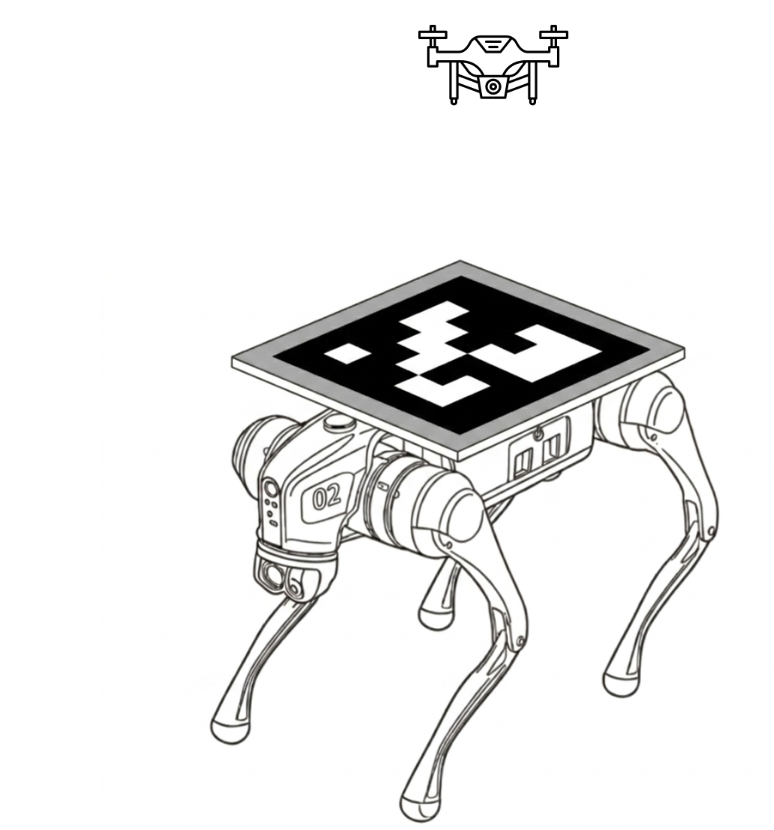
\includegraphics[width=0.52\linewidth]{figures/images/esquema-go2-aruco-dron.png}
\caption{Esquema conceptual del setup experimental base: Go2 instrumentado con
tablero y marcador ArUco sobre el torso, junto con un dron ubicado por encima
como referencia del escenario de observación aérea.}
\label{fig:intro_go2_aruco_drone_scheme}
\end{figure}

\begin{figure}[H]
\centering
\begin{tikzpicture}[x=1cm,y=1cm]
\draw[fill=gray!10,draw=black!60,thick] (-2.2,-0.55) -- (1.9,-0.25) -- (2.25,0.55) -- (-1.85,0.25) -- cycle;
\draw[fill=gray!18,draw=black!55] (-1.85,0.25) -- (2.25,0.55) -- (2.25,0.85) -- (-1.85,0.55) -- cycle;
\draw[fill=gray!22,draw=black!50] (1.9,-0.25) -- (2.25,0.55) -- (2.25,0.85) -- (1.9,0.05) -- cycle;
\draw[-latex,blue!70!black,thick] (0,0.15) -- (0,1.9) node[above]{\small heave};
\draw[-latex,blue!70!black,thick] (0,0.15) -- (2.9,0.38) node[right]{\small surge};
\draw[-latex,blue!70!black,thick] (0,0.15) -- (-1.25,-1.35) node[below]{\small sway};
\draw[-latex,orange!80!black,thick] (-0.95,-1.32) arc[start angle=240,end angle=40,radius=0.54];
\node[orange!80!black] at (-2.25,-0.94) {\small pitch};
\draw[-latex,orange!80!black,thick] (2.6,0.05) arc[start angle=-15,end angle=105,radius=0.55];
\node[orange!80!black] at (3.25,0.78) {\small roll};
\draw[-latex,orange!80!black,thick] (0.62,1.1) arc[start angle=35,end angle=325,radius=0.46];
\node[orange!80!black] at (1.35,1.18) {\small yaw};
\draw[blue!40!black,very thick] (-3.0,-0.88) sin (-2.3,-0.62) cos (-1.6,-0.88) sin (-0.9,-1.14) cos (-0.2,-0.88) sin (0.5,-0.62) cos (1.2,-0.88) sin (1.9,-1.14) cos (2.6,-0.88);
\end{tikzpicture}
\caption{Convención de movimientos marinos usada en el trabajo. Se muestran los
seis grados de libertad de una plataforma; esta etapa prioriza
\textit{roll}, \textit{pitch} y \textit{heave} por su efecto directo sobre la
observación visual del marcador.}
\label{fig:roll_pitch_heave}
\end{figure}

Como se observa en la Figura~\ref{fig:roll_pitch_heave}, el movimiento de una
plataforma marina puede describirse, en general, mediante seis grados de
libertad. En el alcance actual del trabajo no buscamos reproducir
esa dinámica completa, sino aislar las perturbaciones que más directamente
afectan la pose observada del marcador. En nuestro setup, roll y pitch cambian
la orientación aparente del plano del ArUco respecto de la cámara, mientras que
heave modifica la distancia relativa y, con ello, su escala proyectada en la
imagen. En cambio, las componentes horizontales y la rotación en yaw no se
priorizan en esta etapa porque la simulación las mantiene anuladas para validar
primero la cadena movimiento--percepción--evaluación sobre el subconjunto de
variaciones visuales más influyentes.

La primera parte del framework se desarrolló íntegramente en simulación sobre
ROS2 Humble y Gazebo Classic. Allí construimos un pipeline que integra la
generación del movimiento marino, la observación visual del marcador y la
evaluación posterior contra ground truth. El movimiento del torso del Go2 se
controla publicando consignas posturales que inducen oscilaciones periódicas en
roll, pitch y heave. Sobre ese escenario incorporamos dos fuentes de imagen
complementarias. La primera es una cámara fija nadir, útil para estudiar el
problema en un caso controlado donde toda la variabilidad proviene del
movimiento de la plataforma. La segunda es la cámara bottom de un dron
\texttt{sjtu\_drone}, que introduce un escenario más cercano a la aplicación
final, ya que la percepción depende tanto del movimiento del objetivo como de
la pose del vehículo aéreo.

\begin{figure}[H]
\centering
\begin{minipage}[t]{0.49\textwidth}
\centering
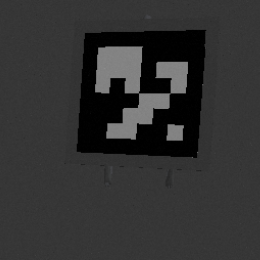
\includegraphics[width=\linewidth]{figures/images/fig_sim_fixed_camera_cropped.png}
\end{minipage}
\hfill
\begin{minipage}[t]{0.49\textwidth}
\centering
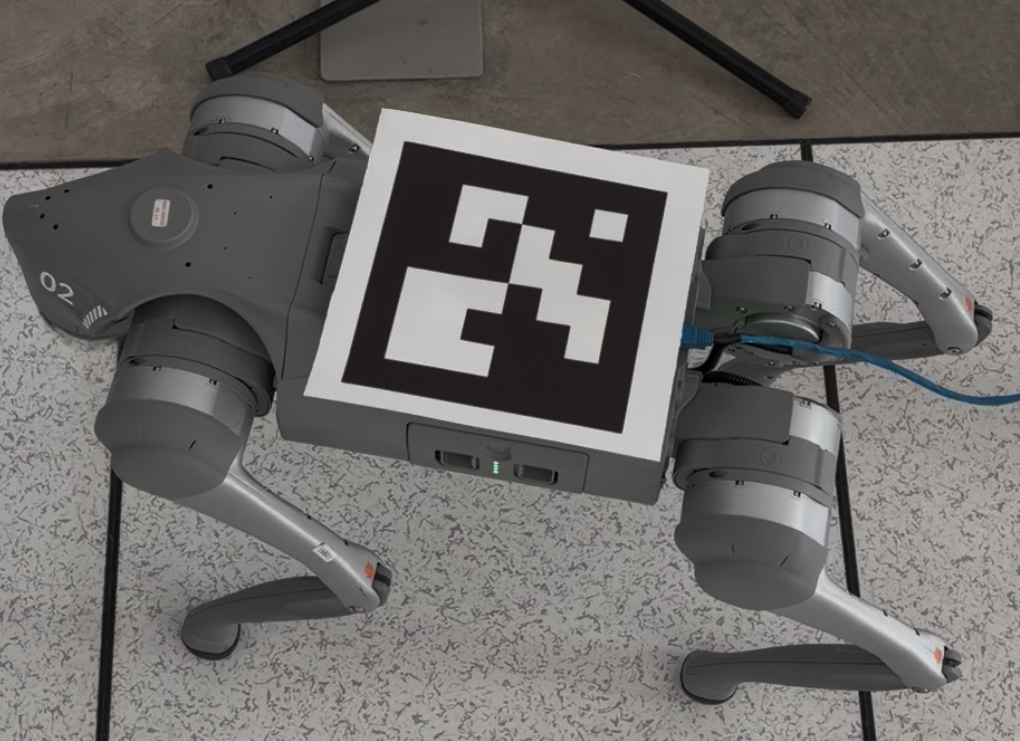
\includegraphics[width=\linewidth]{figures/images/go2_aruco_lab.png}
\end{minipage}
\caption{Vista panorámica del recorrido metodológico de este trabajo. A la izquierda,
una vista representativa del entorno de simulación con el Go2 instrumentado con
ArUco; a la derecha, el traslado al laboratorio con el Go2 real, marcador sobre
el lomo y cámara mantenida en posición aproximadamente fija.}
\label{fig:intro_framework_overview}
\end{figure}

\subsection{Pipeline de percepción y evaluación}

En ambos casos, la estimación visual se resolvió mediante un pipeline basado en
marcadores ArUco y \texttt{solvePnP}. Este último es el procedimiento geométrico
que permite recuperar la pose relativa del marcador a partir de sus esquinas
detectadas y de la calibración de la cámara. El sistema detecta en tiempo real
el marcador montado sobre el robot y estima su pose relativa respecto del frame
óptico de la cámara. Sin embargo, esa estimación online no agota el valor del
framework. Una parte central del trabajo consiste en registrar cada corrida y
comparar después la pose estimada con una referencia obtenida a partir del
estado del simulador. De este modo, este trabajo no se limita a producir una
detección visual funcional, sino que propone un entorno donde la calidad de esa
estimación puede medirse de manera reproducible y con acceso a ground truth.

La segunda parte del trabajo traslada esta lógica al laboratorio. Una vez
establecida la metodología en simulación, utilizamos el Go2 real para
reproducir el movimiento propuesto y analizar qué ocurre cuando se abandona el
entorno idealizado de Gazebo. En esta etapa volvimos a montar un marcador ArUco
sobre el robot y utilizamos una cámara mantenida en posición aproximadamente
fija para observar el movimiento. El propósito ya no fue disponer del tipo de
referencia perfecta que ofrece la simulación, sino estudiar la relación entre
el movimiento deseado y las señales efectivamente publicadas por el cuadrúpedo,
con el fin de evaluar si la síntesis de oleaje planteada en el entorno virtual
mantiene correlación con el comportamiento físico del sistema. Esta transición
entre simulación y laboratorio convierte al framework en algo más que una
herramienta de software: lo acerca a una metodología de validación para futuros
ensayos sobre hardware.

\subsection{Aportes y organización del trabajo}

En este marco, el aporte de este trabajo puede entenderse en cuatro planos. En
primer lugar, desarrollamos un entorno de simulación que reutiliza un
cuadrúpedo como soporte para emular movimiento marino relevante para percepción
visual. En segundo lugar, integramos un pipeline de estimación de pose basado
en ArUco que puede operar tanto con una cámara fija como con una cámara montada
en un dron simulado. En tercer lugar, incorporamos un esquema de registro y
evaluación offline que permite contrastar la estimación contra ground truth en
simulación. Finalmente, extendimos el trabajo al laboratorio para comenzar a
analizar el vínculo entre la plataforma marina sintetizada y el comportamiento
real del robot. Estos aportes no constituyen todavía un sistema completo de
aterrizaje autónomo, pero sí construyen una base experimental y metodológica
para estudiar ese problema con menor riesgo y mayor trazabilidad.

Las dos preguntas de validación recién formuladas también organizan el recorrido
del documento. El Capítulo~\ref{sec:estado_arte} revisa antecedentes de
aterrizaje sobre plataformas móviles, operación marina, marcadores fiduciales y
validación en simulación. El Capítulo~\ref{mt} presenta el marco teórico y los
conceptos necesarios para entender el ecosistema experimental basado en ROS2 y
Gazebo, el modelado del movimiento marino, el uso postural del cuadrúpedo y la
estimación visual con marcadores fiduciales. Luego describimos la metodología
adoptada, distinguiendo la etapa de simulación de la etapa de laboratorio.
Sobre esa base, presentamos la experimentación realizada y discutimos los
hallazgos obtenidos en cada entorno. Finalmente, cerramos con las conclusiones
del trabajo y con las líneas de trabajo futuro que permitirían extender este
framework hacia ensayos más cercanos al aterrizaje autónomo sobre plataformas
marinas.



\section{Estado del arte} \label{sec:estado_arte}

\subsection{Aterrizaje autónomo sobre plataformas móviles}

El aterrizaje autónomo de vehículos aéreos no tripulados sobre plataformas
móviles combina percepción, estimación de movimiento y control en la fase más
riesgosa de una misión. En los primeros antecedentes modernos, el problema se
formuló principalmente como seguimiento visual de un blanco móvil. Lee, Ryan y
Kim propusieron un esquema de servo visual basado en imagen para que un VTOL
siguiera y aterrizara sobre una plataforma en movimiento, generando comandos de
velocidad a partir del error visual en la imagen \citep{Lee2012}. Ese enfoque
instaló una idea que reaparece en buena parte de la literatura posterior: la
cámara no sólo detecta el objetivo, sino que participa directamente en el lazo
de control.

Otros trabajos avanzaron sobre el diseño de blancos visuales y la estimación de
pose relativa. Araar, Aouf y Vitanov estudiaron el aterrizaje de multirrotores
sobre plataformas móviles mediante una landing pad diseñada para facilitar la
estimación visual, combinando percepción e información inercial
\citep{Araar2017}. Falanga y colaboradores, por su parte, mostraron un sistema
capaz de aterrizar sobre una plataforma móvil usando sensado y cómputo a bordo,
con detección y estimación del movimiento de la plataforma integradas en una
arquitectura autónoma \citep{Falanga2017}. En conjunto, estos antecedentes
muestran que el problema no se reduce al último instante de contacto: requiere
localizar la plataforma, seguirla, mantenerla dentro del campo visual y
coordinar la maniobra de aproximación.

La línea más reciente mantiene esa estructura, pero presta mayor atención a la
reproducibilidad y a la validación progresiva. Keipour y colaboradores
propusieron un controlador de servo visual para aterrizar sobre un vehículo en
movimiento usando cámara monocular, un sensor de distancia y cómputo a bordo,
con pruebas en simulación, interiores y exteriores \citep{Keipour2022}. Este
tipo de trabajo es importante porque no presenta la simulación como un recurso
menor, sino como una etapa explícita antes de los ensayos físicos. Aun así, en
estos antecedentes el escenario móvil suele ser terrestre o genérico; la
dinámica marina aparece sólo de forma indirecta, si aparece.

\subsection{Operación marina y cubiertas oscilantes}

Cuando la plataforma objetivo se ubica en un entorno marítimo, el problema
cambia cualitativamente. Ya no alcanza con seguir una traslación horizontal: la
cubierta puede oscilar, inclinarse y modificar su apariencia de manera continua
por efecto del oleaje. Sánchez-López y colaboradores abordaron explícitamente
el aterrizaje visual sobre una cubierta de barco y emularon la dinámica de la
cubierta mediante una plataforma física de seis grados de libertad,
considerando distintos estados de mar y tipos de buque
\citep{SanchezLopez2014}. Ese antecedente es central porque muestra una forma
temprana de validación sustitutiva: antes de operar sobre una embarcación real,
la cubierta se reproduce en un banco experimental controlado.

En trabajos más recientes, Delbene, Baglietto y Simetti propusieron el
aterrizaje autónomo de un UAV sobre un catamarán en entorno marino mediante una
arquitectura que combina visión, AprilTags, ultrasonido y una etapa
software-in-the-loop alimentada con movimientos reales del vehículo de
superficie \citep{Delbene2022}. Cho y colaboradores, en cambio, estudiaron el
aterrizaje sobre una cubierta de barco sometida a movimiento y oscilación por
oleaje, extendiendo el servo visual basado en imagen con estimación de
velocidad del barco, compensación de forma visual y un procedimiento completo
de aproximación y touchdown \citep{Cho2022}. Estos trabajos acercan el problema
al mar real, donde roll, pitch y heave dejan de ser detalles de modelado y
pasan a ser perturbaciones centrales para la percepción y el control.

También existen soluciones que resuelven el aterrizaje preciso desde una
filosofía distinta. Alarcón y colaboradores presentaron un sistema de
aterrizaje GNSS-free sobre plataformas móviles que estima la posición relativa
mediante los ángulos de un cable físico entre UAV y plataforma
\citep{Alarcon2019}. Su valor para esta revisión está en el contraste:
demuestra que la literatura sobre plataformas móviles no es homogénea y que
algunas soluciones alcanzan alta precisión evitando por completo el problema de
la percepción visual. Para un framework centrado en visión, esa diferencia
ayuda a delimitar el alcance: interesa validar cuándo la pose puede recuperarse
desde imagen, no sólo resolver el aterrizaje por cualquier medio disponible.

\subsection{Estimación de pose con marcadores fiduciales}

Una parte importante de los sistemas de aterrizaje visual se apoya en
marcadores artificiales, porque introducen en la escena un patrón de geometría
conocida que puede detectarse de manera robusta. La familia ArUco fue
formalizada por Garrido-Jurado y colaboradores como un sistema de generación y
detección de marcadores cuadrados confiables bajo oclusión
\citep{GarridoJurado2014}. Posteriormente, Romero-Ramírez, Muñoz-Salinas y
Medina-Carnicer propusieron mejoras orientadas a acelerar la detección de
marcadores cuadrados, un aspecto relevante cuando la estimación debe operar en
tiempo real \citep{RomeroRamirez2018}.

La familia AprilTag cumple un rol análogo y aparece en varios trabajos de
robótica móvil y aterrizaje. Olson presentó AprilTag como un sistema fiducial
capaz de recuperar localización 6-DoF desde una imagen \citep{Olson2011};
Wang y Olson mejoraron luego el detector para aumentar eficiencia y robustez,
especialmente en condiciones donde el tamaño aparente del tag es reducido
\citep{WangOlson2016}. La elección entre ArUco, AprilTag u otros patrones no es
un detalle menor: afecta la distancia de detección, la sensibilidad a
oclusiones, el costo computacional y la precisión de las esquinas que luego
alimentan la estimación geométrica.

La detección del marcador, sin embargo, no es lo mismo que la estimación de
pose. Una vez detectadas las esquinas del patrón, la pose relativa se obtiene
resolviendo un problema Perspective-\(n\)-Point con la calibración de cámara y
el tamaño físico del marcador. La familia de métodos PnP, incluyendo EPnP
\citep{Lepetit2009}, aporta el puente geométrico entre correspondencias 2D--3D
y una transformación rígida cámara--objeto. Esta distinción es clave para
ordenar el estado del arte: algunos antecedentes evalúan el éxito del
aterrizaje completo, otros la detección del patrón, y otros la exactitud de la
pose estimada. Esas métricas no son equivalentes.

\subsection{Simulación, SIL y validación previa al ensayo real}

La simulación ocupa un lugar creciente en la literatura porque permite
desacoplar subproblemas, repetir condiciones y reducir el riesgo de ensayos
tempranos. En el caso marino, Sánchez-López y colaboradores ya habían usado una
plataforma física de seis grados de libertad para emular una cubierta antes de
operar en el mar \citep{SanchezLopez2014}. Delbene y colaboradores adoptaron un
enfoque software-in-the-loop con Gazebo y ROS2 para integrar percepción y
control alrededor de un catamarán, reutilizando telemetría real para excitar el
escenario simulado \citep{Delbene2022}. Keipour y colaboradores también
expusieron simulación, ensayos interiores y ensayos exteriores como niveles de
validación progresiva \citep{Keipour2022}.

Desde el punto de vista de infraestructura, Nguyen y Nguyen muestran que la
combinación de Gazebo, PX4 y software-in-the-loop es una base habitual para
probar algoritmos visuales en UAVs antes de trasladarlos a hardware
\citep{Nguyen2019}. La tendencia general es clara: los entornos simulados no se
usan solamente para depurar código, sino para construir evidencia previa sobre
percepción, control y condiciones de falla. La dificultad está en que muchos
trabajos reportan métricas finales de aterrizaje o éxito de misión, pero no
siempre aíslan la exactitud geométrica del estimador de pose frente a una
referencia limpia y repetible.

\subsection{Síntesis crítica y ubicación de este trabajo}

El panorama revisado permite separar tres familias de aportes. Una primera
familia resuelve el aterrizaje completo sobre plataformas móviles y evalúa el
sistema por éxito de aproximación o touchdown
\citep{Lee2012,Araar2017,Falanga2017,Keipour2022}. Una segunda familia se
concentra en el caso marino y reconoce que la cubierta oscilante introduce
perturbaciones específicas sobre la percepción y el control
\citep{SanchezLopez2014,Delbene2022,Cho2022}. Una tercera familia aporta las
herramientas de percepción marker-based y estimación PnP que permiten recuperar
pose relativa desde imagen
\citep{GarridoJurado2014,RomeroRamirez2018,Olson2011,WangOlson2016,Lepetit2009}.

La intersección entre esas familias sigue siendo menos poblada: no abundan los
marcos pensados específicamente para validar cuantitativamente un estimador de
pose visual, basado en marcador fiducial, bajo movimientos marinos sintetizados
y con comparación directa contra ground truth del simulador. Este trabajo se
ubica en esa zona metodológica. No compite con los sistemas que ya cierran el
lazo de aterrizaje completo; construye una etapa previa para estudiar si la
pose visual de una plataforma oscilante puede estimarse, registrarse y
compararse de manera reproducible antes de avanzar hacia ensayos de mayor
riesgo.

\section{Marco teórico} \label{mt}

\subsection{Introducción conceptual}

Cuando se piensa en el aterrizaje de un dron sobre una superficie en
movimiento, la dificultad más evidente parece ser visual: detectar la
plataforma y conocer su pose relativa con suficiente precisión. Sin embargo,
esa dificultad es apenas el último eslabón de una cadena más amplia. Antes de
que una cámara recupere una pose, existe una superficie que se traslada y se
inclina; y antes de que ese movimiento pueda medirse, hace falta una
descripción física que permita distinguir qué componentes son relevantes, cómo
evolucionan y de qué manera afectan la observación. En línea con esa
perspectiva, trabajos recientes sobre aterrizaje autónomo en plataformas
móviles y marinas abordan de forma articulada la dinámica de la plataforma, la
estimación visual de su estado y las decisiones de control del vehículo
\citep{Alarcon2019,Delbene2022,Morales2023}. Retomamos esa misma lógica para
organizar este marco teórico: partir del ecosistema experimental que vuelve
observable y registrable el problema, describir luego el movimiento que
queremos sintetizar, y recién entonces vincularlo con la plataforma robótica y
con la percepción visual.

En nuestro caso, esa cadena recorre cinco niveles acoplados. El primero es de
infraestructura: hace falta un entorno de simulación y comunicación que permita
coordinar sensores, marcos de referencia y registros reproducibles. El
segundo es físico: caracterizar un movimiento semejante al de una plataforma
marina y reducirlo a las componentes que más perturban la observación del
marcador. El tercero es mecánico: traducir esa descripción a un sistema
robotizado capaz de reproducir de manera repetible inclinaciones y
desplazamientos verticales. El cuarto es geométrico: organizar marcos y
transformaciones para relacionar el torso del robot, el marcador y la cámara.
El quinto es visual: relacionar la pose tridimensional del marcador con su
proyección en la imagen y reconstruirla a partir de un modelo de cámara
calibrada. Ninguna de estas piezas es independiente de las otras.

Desde esa perspectiva, el desarrollo teórico avanza en el mismo sentido que el
problema. Primero se introduce el ecosistema experimental basado en ROS2,
Gazebo, transformaciones entre marcos y registros reproducibles, porque es allí
donde el sistema adquiere trazabilidad. Luego se presenta una representación
simplificada del movimiento marino que
preserve las perturbaciones dominantes del escenario. Sobre esa base se
describe la elección del Unitree Go2 como plataforma marina sintética y la
instrumentación visual con cámara fija, dron y marcador fiducial. Después se
discute cómo el cuadrúpedo materializa una consigna postural y cómo se ordenan
los marcos de referencia necesarios para comparar estimación y ground truth.
Finalmente, se presentan las herramientas de marcadores ArUco, geometría
proyectiva y \texttt{solvePnP} que permiten pasar de la imagen a una
descripción métrica de la pose relativa.

\subsection{Ecosistema experimental: ROS2, Gazebo y registro reproducible}

El framework no se apoya solamente en un modelo físico o en un detector visual,
también necesita una infraestructura de software capaz de coordinar control,
sensado, estimación y evaluación. En este trabajo esa infraestructura está dada
por ROS2 y Gazebo Classic. ROS2 funciona como \emph{middleware} del sistema: en
lugar de concebir el experimento como un programa monolítico, lo organizamos
como un grafo de procesos especializados que intercambian información mediante
publicación y suscripción tipada \citep{ros2_basic_concepts}. Esta decisión no
es un detalle de implementación. Es la que permite desacoplar la generación del
movimiento, la fuente de imagen, la estimación visual y el análisis posterior,
sin perder coherencia entre ellas.

En este contexto, el \emph{grafo} de ROS2 puede pensarse como un mapa de qué
componentes están activos y cómo se conectan entre sí. Cada \emph{nodo} es uno
de esos componentes y encapsula una responsabilidad concreta del pipeline: por
ejemplo, generar el movimiento, publicar una imagen, detectar el marcador o
registrar una corrida. Los \emph{tópicos}, en cambio, son canales nombrados por
los que esos nodos intercambian mensajes de un tipo bien definido. Un nodo
puede publicar en un tópico si produce una señal, o suscribirse a él si la
necesita para seguir procesando. Así, la imagen de la cámara, la consigna
postural del robot, la pose estimada del marcador o las señales de depuración
circulan como piezas distintas pero compatibles dentro de una misma red.

La utilidad de esta organización es doble. Por un lado, permite construir el
experimento como una cadena modular en la que cada parte puede inspeccionarse o
reemplazarse sin reescribir todo el sistema. Por otro, vuelve explícito quién
produce cada dato, quién lo consume y en qué punto del pipeline se genera una
corrida determinada. Esa trazabilidad es especialmente importante en este trabajo,
porque más adelante necesitamos comparar lo que publica el detector visual con
lo que registra el simulador y con lo que queda almacenado para la evaluación
\textit{offline}.

Además de intercambiar mensajes, el sistema debe mantener consistencia
geométrica entre referencias que no coinciden entre sí. La cámara, el torso del
robot, el marcador y el mundo no comparten el mismo origen ni la misma
orientación. En ROS2, esa relación se organiza mediante \emph{TF}/\emph{tf2},
una biblioteca que mantiene a lo largo del tiempo una estructura de
transformaciones entre marcos de referencia y permite convertir poses, puntos y
vectores entre ellos \citep{tf2_humble}. Esta capa es crucial porque hace
posible hablar de la misma escena desde el frame del robot, desde el de la
cámara o desde un frame global sin mezclar descripciones incompatibles.

Gazebo Classic aporta la otra mitad del ecosistema: el entorno de simulación
física y sensorial. Conceptualmente, Gazebo integra la evolución dinámica del
mundo con la generación de sensores, el renderizado y la interfaz de
visualización \citep{gazebo_classic_architecture}. Para este trabajo eso resulta
especialmente valioso porque la postura del Go2, la imagen observada por la
cámara y gran parte del ground truth provienen de un mismo estado subyacente
del simulador. No trabajamos, entonces, con una animación separada de los
datos, sino con un entorno donde la escena visual y las señales del sistema
quedan ligadas a la misma evolución temporal.

Finalmente, la reproducibilidad del framework depende del registro. Un
\emph{rosbag} es un registro persistente de los datos intercambiados por el
sistema, que puede reproducirse e inspeccionarse después sin volver a ejecutar
la simulación \citep{ros2_rosbag2_tutorial}. En nuestro caso, esto permite
separar la estimación en tiempo real del análisis offline, revisar una misma
secuencia con distintos criterios y comparar la pose estimada del marcador con
una referencia reconstruida a partir del estado del simulador. En otras
palabras, ROS2, Gazebo, TF y los rosbags no son accesorios del experimento:
constituyen la base que vuelve trazable y repetible el problema que queremos
estudiar.

\subsection{Movimiento marino simplificado}

El punto de partida del problema es físico antes que computacional. Una
plataforma apoyada sobre el mar no responde al paso de una ola únicamente
subiendo y bajando. A medida que la superficie libre se eleva y cambia su
pendiente, la cubierta también puede inclinarse. Si toda la plataforma asciende
o desciende de forma aproximadamente uniforme, domina el movimiento vertical
\emph{heave}. Si proa y popa quedan apoyadas sobre alturas distintas, aparece
\emph{pitch}. Si la diferencia de altura se produce entre babor y estribor,
aparece \emph{roll}. En una embarcación real estos efectos coexisten y se
combinan con otras componentes horizontales, pero esta lectura inicial permite
entender por qué el oleaje no se traduce en una sola perturbación sino en una
roto-traslación completa de la plataforma.

\begin{figure}[H]
\centering
\begin{minipage}[t]{0.31\textwidth}
\centering
\begin{tikzpicture}[x=0.7cm,y=0.7cm]
\draw[dashed,gray] (-0.2,0.55) -- (5.4,0.55);
\draw[blue!70!black,thick,smooth] plot coordinates {(0,0.15) (1,0.65) (2,1.15) (3,0.95) (4,0.35) (5,0.2)};
\draw[fill=black!15,thick] (1.6,1.35) -- (3.6,1.35) -- (3.2,0.9) -- (2.0,0.9) -- cycle;
\draw[fill=gray!35,thick] (2.45,1.35) rectangle (2.8,1.75);
\draw[latex-latex,red!75!black,thick] (4.55,0.55) -- (4.55,1.35);
\node[red!75!black,right] at (4.65,0.95) {\scriptsize heave};
\end{tikzpicture}
\end{minipage}
\hfill
\begin{minipage}[t]{0.31\textwidth}
\centering
\begin{tikzpicture}[x=0.7cm,y=0.7cm]
\draw[dashed,gray] (-0.2,0.55) -- (5.4,0.55);
\draw[blue!70!black,thick,smooth] plot coordinates {(0,0.0) (1,0.35) (2,0.85) (3,1.25) (4,1.1) (5,0.7)};
\begin{scope}[rotate around={12:(2.6,1.4)}]
\draw[fill=black!15,thick] (1.4,1.4) -- (3.8,1.4) -- (3.35,0.95) -- (1.95,0.95) -- cycle;
\draw[fill=gray!35,thick] (2.45,1.4) rectangle (2.8,1.8);
\end{scope}
\draw[latex-,orange!85!black,thick] (4.45,1.0) arc[start angle=-35,end angle=18,radius=0.45];
\node[orange!85!black,right] at (4.95,1.28) {\scriptsize pitch};
\end{tikzpicture}
\end{minipage}
\hfill
\begin{minipage}[t]{0.31\textwidth}
\centering
\begin{tikzpicture}[x=0.7cm,y=0.7cm]
\draw[dashed,gray] (-0.2,0.55) -- (5.4,0.55);
\draw[blue!70!black,thick,smooth] plot coordinates {(0,0.05) (1,0.3) (2,0.8) (3,1.15) (4,1.45) (5,1.6)};
\begin{scope}[rotate around={-11:(2.7,1.4)}]
\draw[fill=black!15,thick] (1.45,1.4) -- (3.95,1.4) -- (3.45,0.95) -- (1.95,0.95) -- cycle;
\draw[fill=gray!35,thick] (2.5,1.4) rectangle (2.85,1.8);
\end{scope}
\draw[latex-,teal!70!black,thick] (4.45,1.55) arc[start angle=155,end angle=95,radius=0.45];
\node[teal!70!black,right] at (4.95,1.78) {\scriptsize roll};
\end{tikzpicture}
\end{minipage}
\caption{Interpretación física simplificada del movimiento de una plataforma
sobre las olas. De izquierda a derecha: elevación local de la superficie
libre, que induce \emph{heave}; diferencia de altura entre proa y popa, que
induce \emph{pitch}; y diferencia de altura entre babor y estribor, que induce
\emph{roll}.}
\label{fig:wave_platform_response}
\end{figure}

La formulación clásica de dinámica marina describe el movimiento de una
embarcación mediante seis grados de libertad \citep{Fossen1995}. Tres de ellos
son traslacionales: \emph{surge}, \emph{sway} y \emph{heave}. Los otros tres
son rotacionales: \emph{roll}, \emph{pitch} y \emph{yaw}. Si reunimos posición
y orientación en el vector
\(\eta = [x \;\; y \;\; z \;\; \phi \;\; \theta \;\; \psi]^\top\), y las
velocidades lineales y angulares en el frame del cuerpo en
\(\nu = [u \;\; v \;\; w \;\; p \;\; q \;\; r]^\top\), una forma compacta de la
cinemática es

\begin{equation}
\dot{\eta} = J(\eta)\,\nu,
\label{eq:marine_kinematics}
\end{equation}

donde \(J(\eta)\) transforma velocidades expresadas en el cuerpo en derivadas
de posición y orientación respecto del frame inercial. Esta ecuación resume una
idea importante: la pose de la plataforma no cambia de manera arbitraria, sino
como resultado de un acoplamiento entre traslaciones, rotaciones y la
orientación instantánea del casco.

En un modelo dinámico completo, además, ese movimiento surge del equilibrio
entre inercia, amortiguamiento, gravedad, flotación y excitación externa. Una
escritura habitual es

\begin{equation}
M \dot{\nu} + C(\nu)\nu + D(\nu)\nu + g(\eta) = \tau + \tau_w,
\label{eq:marine_dynamics}
\end{equation}

donde \(M\) representa la inercia, \(C(\nu)\nu\) los términos de Coriolis,
\(D(\nu)\nu\) el amortiguamiento hidrodinámico, \(g(\eta)\) las fuerzas
restauradoras asociadas a gravedad y flotación, \(\tau\) posibles acciones de
control y \(\tau_w\) la excitación inducida por el mar. El objetivo de este
trabajo no es resolver este modelo con fidelidad hidrodinámica completa, sino
usar esta formulación para entender qué parte del movimiento conviene retener
cuando el interés principal es describir la oscilación local de una plataforma.

Para conectar el oleaje con la postura de la cubierta, resulta útil introducir
la elevación de la superficie libre \(\zeta(x,y,t)\), medida respecto del nivel
medio del mar. Si \((x_p,y_p)\) denota la posición horizontal de referencia de
la plataforma y se adopta una aproximación local de primer orden, entonces una
lectura simplificada del movimiento retenido puede escribirse como

\begin{equation}
\eta_r(t) \approx
\begin{bmatrix}
z(t) \\
\phi(t) \\
\theta(t)
\end{bmatrix}
=
\begin{bmatrix}
\zeta(x_p,y_p,t) \\
\kappa_{\phi}\,\dfrac{\partial \zeta}{\partial y}(x_p,y_p,t) \\
-\kappa_{\theta}\,\dfrac{\partial \zeta}{\partial x}(x_p,y_p,t)
\end{bmatrix},
\label{eq:reduced_marine_state}
\end{equation}

donde \(z\) representa el movimiento vertical, \(\phi\) el \emph{roll},
\(\theta\) el \emph{pitch}, y \(\kappa_{\phi}\), \(\kappa_{\theta}\) resumen de
forma agregada cuánto acompaña la plataforma la pendiente local de la
superficie. Esta ecuación no pretende ser un modelo naval exhaustivo. Su valor
teórico está en capturar la intuición correcta: la elevación local del agua
explica el ascenso y descenso de la plataforma, mientras que la pendiente de la
ola explica su inclinación.

Esta lectura también permite entender por qué la posición de la plataforma
sobre la ola modifica cualitativamente su movimiento. Como la superficie libre
se comporta como una onda, no todas sus regiones tienen la misma altura ni la
misma pendiente al mismo tiempo. Si el centro de la plataforma coincide con una
cresta o con un valle, la elevación local puede ser extrema, pero la pendiente
alrededor de ese punto tiende a ser menor; en ese caso domina el movimiento
vertical. En cambio, cuando la plataforma se ubica sobre el flanco de la onda,
la elevación puede ser intermedia, pero la pendiente es mayor y, por lo tanto,
crecen las inclinaciones. En otras palabras, no alcanza con saber que ``hay una
ola'': también importa en qué fase espacial de esa ola se encuentra la
plataforma y cómo esa fase cambia a medida que la onda se propaga.

Una forma todavía más concreta de verlo es comparar la altura del agua en
distintos puntos de la plataforma. Si \(\zeta_{\text{proa}}\),
\(\zeta_{\text{popa}}\), \(\zeta_{\text{babor}}\) y
\(\zeta_{\text{estribor}}\) representan la elevación local del agua bajo esas
cuatro zonas características, entonces una aproximación elemental es

\begin{equation}
\begin{aligned}
z(t) &\approx \frac{\zeta_{\text{proa}} + \zeta_{\text{popa}} +
\zeta_{\text{babor}} + \zeta_{\text{estribor}}}{4}, \\
\theta(t) &\propto \frac{\zeta_{\text{proa}} - \zeta_{\text{popa}}}{L_p}, \\
\phi(t) &\propto \frac{\zeta_{\text{estribor}} - \zeta_{\text{babor}}}{B_p},
\end{aligned}
\label{eq:platform_finite_difference_response}
\end{equation}

La Figura~\ref{fig:platform_corner_heights} resume gráficamente esta
aproximación discreta del movimiento de la plataforma a partir de alturas
locales del agua medidas en zonas representativas de la cubierta.

\figureplaceholder{fig:platform_corner_heights}{Figura pendiente del efecto del
oleaje sobre una embarcación vista en perspectiva oblicua. La imagen final
debería mostrar una lancha o pequeño barco sobre una superficie ondulada, con
una geometría clara y simple, sin exceso de texto dentro del dibujo. Deben
identificarse cuatro zonas representativas de la cubierta ---proa, popa,
babor y estribor--- y sugerirse visualmente cómo las diferencias de altura del
agua bajo esos puntos se traducen en \emph{heave}, \emph{pitch} y
\emph{roll}. Idealmente, la figura debería privilegiar la intuición física:
barco más olas, pocos rótulos y composición limpia.}{Esquema pendiente del
efecto del oleaje sobre una embarcación y su relación con la aproximación
discreta de \emph{heave}, \emph{pitch} y \emph{roll}.}

En esta lectura, \(L_p\) y \(B_p\) representan, respectivamente, una longitud
característica en la dirección proa--popa y una manga efectiva en la dirección
babor--estribor. Estas relaciones no reemplazan al modelo dinámico completo,
pero hacen explícita una idea central para este trabajo: el movimiento de la
plataforma no depende solamente de la amplitud de la ola, sino también de la
posición y de la extensión espacial de la superficie que esa ola está
excitando.

Esa relación también justifica el recorte adoptado en este trabajo. En un
escenario real, \emph{surge}, \emph{sway} y \emph{yaw} pueden ser relevantes;
sin embargo, cuando el interés se centra en una plataforma que mantiene su
posición horizontal de manera aproximada y lo que se busca es sintetizar la
oscilación local de la cubierta, las componentes más representativas pasan a
ser justamente \emph{heave}, \emph{roll} y \emph{pitch}. Esas tres variables
resumen la parte del movimiento que una ola transmite de forma más directa a la
superficie sobre la que, en una etapa posterior del proyecto, debería
posicionarse un vehículo aéreo.

Una forma elemental de representar un oleaje regular es mediante una onda
sinusoidal:

\begin{equation}
\zeta(x,y,t) = A \sin(k_x x + k_y y - \omega t + \delta),
\label{eq:sinusoidal_wave_model}
\end{equation}

donde \(A\) es la amplitud, \((k_x,k_y)\) fija la dirección espacial de
propagación, \(\omega\) es la frecuencia angular y \(\delta\) el desfase
inicial. Esta expresión es útil porque permite describir de manera simple una
ola periódica y, al mismo tiempo, deja claro de qué parámetros depende la
respuesta de la plataforma: cuánto sube y baja, con qué rapidez oscila y cómo
se distribuye la pendiente de la superficie.

Cuando se desea representar un mar menos regular, la misma idea puede
extenderse a una superposición de armónicos:

\begin{equation}
\zeta(x,y,t) = \sum_{n=1}^{N} A_n \sin(k_{x,n} x + k_{y,n} y - \omega_n t + \delta_n),
\label{eq:harmonic_wave_model}
\end{equation}

que puede interpretarse como una aproximación simple a un estado de mar más
irregular. Desde el punto de vista conceptual, la diferencia entre ambos casos
no es menor: el oleaje sinusoidal facilita el análisis porque concentra la
respuesta en una única escala temporal dominante, mientras que la suma de
armónicos introduce una superficie más cambiante y menos predecible, parecida a
la que encontraría una plataforma fuera de condiciones idealizadas.

\begin{figure}[H]
\centering
\begin{minipage}[t]{0.47\textwidth}
\centering
\begin{tikzpicture}[x=0.8cm,y=0.8cm]
\draw[dashed,gray] (-0.2,0.5) -- (7.2,0.5) node[right,black] {\scriptsize nivel medio};
\draw[blue!70!black,thick,smooth] plot coordinates {(0,0.5) (1,1.1) (2,1.45) (3,1.1) (4,0.5) (5,-0.1) (6,-0.45) (7,-0.1)};
\node[black] at (3.5,2.0) {\scriptsize ola regular};
\end{tikzpicture}
\end{minipage}
\hfill
\begin{minipage}[t]{0.47\textwidth}
\centering
\begin{tikzpicture}[x=0.8cm,y=0.8cm]
\draw[dashed,gray] (-0.2,0.5) -- (7.2,0.5) node[right,black] {\scriptsize nivel medio};
\draw[blue!70!black,thick,smooth] plot coordinates {(0,0.35) (0.6,0.95) (1.2,0.8) (2.0,1.4) (2.8,0.6) (3.5,1.0) (4.2,0.1) (5.0,-0.35) (5.8,0.2) (6.5,-0.15) (7.0,0.25)};
\node[black] at (3.5,2.0) {\scriptsize oleaje irregular};
\end{tikzpicture}
\end{minipage}
\caption{Perfiles conceptuales de la superficie libre. A la izquierda, una ola
regular con una escala temporal dominante; a la derecha, una superficie más
irregular representada como combinación de varias componentes.}
\label{fig:wave_regular_irregular}
\end{figure}

El recorte a \emph{heave}, \emph{roll} y \emph{pitch} fija, entonces, qué parte
del movimiento queremos sintetizar y por qué esa parte es suficiente para una
primera validación de percepción visual. Sin embargo, todavía queda abierta una
pregunta clave: qué dispositivo experimental puede materializar ese movimiento
de manera repetible y, al mismo tiempo, ser observado por una cámara con una
geometría controlada. Esa es la función que en nuestro framework cumple el
cuadrúpedo instrumentado.

\subsection{Plataforma robótica e instrumentación visual}

La plataforma elegida para materializar ese movimiento es un robot cuadrúpedo
Unitree Go2. La decisión no se tomó para reutilizar un robot de locomoción en
su uso más habitual, sino para explotarlo de otro modo: como una estructura
articulada capaz de modificar la postura de su torso mientras mantiene los
apoyos en el suelo. En lugar de modelar una embarcación completa, aprovechamos
esa capacidad para pedir inclinaciones y desplazamientos verticales del cuerpo y
usar el torso como plataforma marina sintética. La ventaja adicional es
experimental: el mismo robot existe en simulación y en laboratorio, de modo que
la transición entre ambos entornos conserva la lógica general del sistema.

Sobre el torso montamos una tabla rígida con un marcador fiducial. En términos
generales, un marcador fiducial es un patrón visual diseñado para introducir en
la escena una referencia cuya identidad y geometría puedan recuperarse de forma
confiable desde la imagen. En este trabajo ese patrón cumple una función
precisa: convertir la postura del robot en una pose observable por cámara. Así,
el problema visual ya no consiste en inferir la geometría de una embarcación
compleja, sino en estimar la pose de un objeto plano y bien definido unido
rígidamente al cuerpo del Go2.

La observación del marcador se organiza en dos configuraciones complementarias.
La primera utiliza una cámara fija nadir, que funciona como caso base porque el
sensor permanece inmóvil y toda la variabilidad de la secuencia proviene del
movimiento de la plataforma. En el repositorio, esta configuración aparece en
el paquete \texttt{fixed\_camera}. La segunda utiliza la cámara inferior del
\texttt{sjtu\_drone}, un cuadricóptero simulado que introduce una cámara
embarcada y, por lo tanto, un escenario donde la geometría observada depende
tanto del movimiento del marcador como de la pose del vehículo aéreo. Esta
diferencia es conceptualmente importante: el caso de cámara fija aísla el
efecto del oleaje sintético sobre la observación, mientras que el caso con dron
aproxima el problema al escenario futuro de aterrizaje sobre una plataforma
móvil.

En ambas configuraciones, la percepción se resuelve con un detector visual que
consume imagen e intrínsecos de cámara y produce una pose estimada del marcador
respecto del frame óptico. Desde el punto de vista conceptual, este detector
opera como puente entre dos descripciones distintas de la misma escena: la
física, representada por la postura real o simulada del robot, y la proyectiva,
representada por la imagen que observa la cámara. La metodología detallará qué
nodos implementan cada una de estas funciones, pero el punto teórico es más
simple: el sistema queda organizado como una cadena en la que una plataforma
postural genera un patrón observable y una cámara recupera una pose relativa a
partir de ese patrón.

\subsection{Control postural del Go2 y marcos de referencia}

Una vez definido el movimiento que queremos emular, aparece la pregunta central
de la plataforma experimental: \emph{¿cómo convertir ese movimiento deseado en
una postura físicamente consistente del robot?} La respuesta se apoya en la
cinemática y en la dinámica de un cuadrúpedo en contacto con el suelo. Intuitivamente, el Go2 puede pensarse como un torso rígido sostenido por cuatro patas
articuladas. Si las patas cambian su configuración mientras los apoyos se
mantienen, el torso puede inclinarse o subir y bajar sin necesidad de
desplazarse horizontalmente. Esa es, precisamente, la propiedad que explotamos
en este problema: no se usa al cuadrúpedo como vehículo de locomoción, sino como una
estructura reconfigurable capaz de materializar un movimiento postural
controlado.

En este contexto, la Figura~\ref{fig:theory_motion_components} muestra cómo se
interpretan sobre el propio Go2 las tres componentes retenidas por el
framework. El eje vertical del torso fija la lectura de \emph{heave}, mientras
que las inclinaciones alrededor de los ejes corporales permiten distinguir
\emph{roll} y \emph{pitch} en la plataforma sintética.

\begin{figure}[H]
\centering
\includegraphics[width=0.88\textwidth]{figures/diagrams/translations_rotations.png}
\caption{Convención corporal adoptada para el Go2 como plataforma marina
sintética. El torso del robot sintetiza \emph{heave} como traslación vertical y
\emph{roll}/\emph{pitch} como inclinaciones respecto de sus ejes corporales.
Esta es la lectura específica del cuadrúpedo que después implementa la
consigna postural del sistema.}
\label{fig:theory_motion_components}
\end{figure}

Desde el punto de vista del modelado, un cuadrúpedo es un sistema multicuerpo
con base flotante y restricciones de contacto. Si \(q\) reúne la pose del torso
y todos los ángulos articulares, una forma compacta de sus ecuaciones de
movimiento es

\begin{equation}
M(q)\ddot{q} + h(q,\dot{q}) = S^\top \tau + J_c(q)^\top \lambda,
\label{eq:quadruped_dynamics}
\end{equation}

donde \(M(q)\) es la matriz de inercia, \(h(q,\dot{q})\) agrupa términos de
gravedad, Coriolis y otros efectos no lineales, \(\tau\) es el vector de
torques articulares, \(S\) selecciona las coordenadas actuadas, \(J_c(q)\) es
el Jacobiano de contacto y \(\lambda\) representa las fuerzas de reacción en los
pies \citep{Bellicoso2017,Fahmi2019}. Esta ecuación deja en evidencia una idea
importante: la postura del torso no depende solamente de los motores, sino
también de cómo el robot intercambia fuerzas con el suelo.

Cuando un pie permanece apoyado sin deslizar, su velocidad relativa al suelo
debe anularse. Esa condición de contacto puede expresarse como

\begin{equation}
J_c(q)\dot{q} = 0,
\label{eq:contact_velocity_constraint}
\end{equation}

y, en aceleración, como

\begin{equation}
J_c(q)\ddot{q} + \dot{J}_c(q,\dot{q})\dot{q} = 0.
\label{eq:contact_acceleration_constraint}
\end{equation}

En un problema de locomoción completa estas restricciones conviven con cambios
de apoyo, despegues y redistribución dinámica de cargas. En nuestro caso, en
cambio, la situación es bastante más simple: el framework utiliza al Go2 en un
régimen postural, con movimiento suave y sin perseguir desplazamientos sobre el
plano. Eso permite adoptar una lectura cuasiestática y concentrarnos en cómo una
consigna de pose del cuerpo se transforma en una nueva geometría de patas.

\figureplaceholder{fig:go2_postural_control_scheme}{Figura pendiente de la
geometría postural del Go2. Sería útil mostrar una vista frontal y otra lateral
del robot con las cuatro patas en apoyo, el frame \texttt{base\_link}, la
proyección \texttt{base\_footprint} sobre el suelo y ejemplos de cómo cambios
en altura, roll y pitch alteran la longitud relativa de las patas.}{Esquema
pendiente del principio de control postural que permite utilizar al Go2 como
plataforma marina sintética. Una figura así ayudaría a conectar la intuición
geométrica con las ecuaciones de cinemática del cuadrúpedo.}

Si representamos por \(\{b\}\) el frame del torso, por \(\{w\}\) el frame del
mundo y por \(\{f_i\}\) el punto de contacto del pie \(i\), la posición del pie
en el mundo puede escribirse como

\begin{equation}
{}^{w}\!p_{f_i} =
{}^{w}\!p_b + {}^{w}\!R_b \, {}^{b}\!p_{f_i}(q_i),
\qquad i \in \{1,2,3,4\},
\label{eq:foot_forward_kinematics}
\end{equation}

donde \( {}^{w}\!p_b \) y \( {}^{w}\!R_b \) son la posición y orientación del
torso, \(q_i\) es el vector articular de la pata \(i\), y
\({}^{b}\!p_{f_i}(q_i)\) es la posición del pie expresada en el frame del
cuerpo. Esta relación resume una idea clave: la postura del torso no se controla
de forma aislada, sino a través de la geometría conjunta del cuerpo y de las
cuatro patas. En otras palabras, ordenar un roll o un pitch del torso equivale a
pedir una nueva organización espacial de los cuatro apoyos relativos al cuerpo.

En un régimen de apoyo cuasiestático o de apoyo controlado, si asumimos que los
puntos de contacto se mantienen aproximadamente fijos en el mundo, entonces una
pose deseada del torso determina de manera unívoca qué posiciones deberían
adoptar los pies en el frame del cuerpo:

\begin{equation}
{}^{b}\!p_{f_i}^{\star} =
({}^{w}\!R_b^{\star})^\top
\left({}^{w}\!p_{f_i} - {}^{w}\!p_b^{\star}\right).
\label{eq:desired_foot_positions}
\end{equation}

Esta ecuación es la base cinemática del control postural empleado en robots
cuadrúpedos: en lugar de mandar directamente una embarcación virtual, se manda
una pose del cuerpo y se reconfiguran las patas para realizarla de manera
coherente \citep{Bellicoso2017,Fahmi2019}. Esa misma idea es la que hace
posible utilizar al Go2 como plataforma marina sintética. En nuestro framework
la entrada física relevante no es una secuencia de torques individuales, sino
una consigna postural del torso con \(x=y=0\), yaw nulo y variaciones en
altura, roll y pitch. Conceptualmente, esa consigna no describe directamente la
postura articular de las patas, sino la pose deseada del cuerpo que el stack de
control debe realizar.

También resulta útil introducir una noción elemental de estabilidad. Si los
cuatro pies apoyados definen en el plano una envolvente convexa
\(\mathcal{P}_s\), la proyección horizontal del centro de masa del robot,
\(p_{\text{CoM}}^{xy}\), debería permanecer dentro de esa región para sostener
un equilibrio estático simple:

\begin{equation}
p_{\text{CoM}}^{xy} \in \mathcal{P}_s.
\label{eq:support_polygon_condition}
\end{equation}

Aunque en la simulación no resolvemos explícitamente un problema de estabilidad
con fuerzas de contacto, esta condición ayuda a entender por qué las amplitudes
de roll, pitch y heave deben permanecer acotadas. Si la consigna postural fuera
excesiva, el robot dejaría de comportarse como una plataforma controlada y
aparecerían limitaciones mecánicas o configuraciones poco realistas para el
objetivo del framework.

Además, alrededor de una postura nominal puede obtenerse una lectura física muy
intuitiva mediante una linealización de primer orden. Si \(\delta p_b\) es una
pequeña traslación del torso y \(\delta \omega\) una pequeña rotación, la
variación requerida en la posición del pie \(i\) expresada en el cuerpo se
aproxima por

\begin{equation}
\delta {}^{b}\!p_{f_i}
\approx
-\,\delta p_b
-\,\delta \omega \times {}^{b}\!p_{f_i,0},
\label{eq:body_variation_to_feet}
\end{equation}

donde \( {}^{b}\!p_{f_i,0} \) es la posición nominal del pie. Esta expresión
permite interpretar directamente el efecto de cada grado de libertad: un cambio
simétrico de altura afecta a las cuatro patas de manera parecida y genera
heave; una diferencia entre patas izquierdas y derechas induce roll; y una
diferencia entre patas delanteras y traseras induce pitch. En otras palabras, la
dinámica marina reducida se traduce en una redistribución geométrica de apoyo.
De este modo, cada componente del oleaje sintético puede asociarse con una
modificación física concreta del robot.

Para llevar esa consigna al espacio articular, cada pata satisface una relación
de cinemática diferencial del tipo

\begin{equation}
\delta {}^{b}\!p_{f_i} = J_i(q_i)\,\delta q_i,
\label{eq:leg_jacobian}
\end{equation}

de modo que, cuando el Jacobiano \(J_i\) es invertible o admite una
pseudoinversa adecuada, puede obtenerse

\begin{equation}
\delta q_i = J_i^{\dagger}(q_i)\,\delta {}^{b}\!p_{f_i}.
\label{eq:leg_inverse_differential_kinematics}
\end{equation}

Este paso no solo conecta la pose deseada del torso con los doce actuadores del
Go2, sino que explica por qué el robot puede generar inclinaciones observables
sin necesidad de desplazarse en el plano. Esta propiedad es
fundamental: buscamos una plataforma que perturbe de forma controlada la
geometría vista por la cámara, no un sistema de navegación horizontal completo.
En términos de interpretación, el Jacobiano de cada pata traduce una pequeña
corrección en la ubicación deseada del pie en una pequeña corrección de hombro,
muslo y rodilla. Ese puente entre espacio cartesiano y espacio articular es lo
que vuelve realizable una consigna postural del torso como la que adopta el
framework.

También conviene distinguir los marcos de referencia que reaparecen a lo largo
de todo el pipeline. El frame \texttt{world} \(\{w\}\) funciona como
referencia global de Gazebo. El frame \texttt{base\_footprint} \(\{bf\}\)
resume la referencia del robot sobre el plano de apoyo y puede pensarse como la
``sombra'' del cuadrúpedo sobre el suelo. El frame \texttt{base\_link}
\(\{bl\}\), en cambio, está asociado al torso y es el que transporta
efectivamente el marcador. Sobre esa base se define el frame del ArUco
\(\{a\}\), rígidamente unido a la tabla montada sobre el lomo. Para la cámara,
en cambio, conviene distinguir una cadena propia de frames; sin embargo, la
observación visual y la pose publicada por el detector quedan finalmente
expresadas en el frame óptico \(\{c\}\).
En la notación cinemática de las ecuaciones anteriores, este torso coincide con
el frame cuerpo del robot; aquí adoptamos los nombres ROS porque son los que
reaparecen después en TF y en el postproceso. Esta organización se resume en la
Figura~\ref{fig:theory_frames_overview}.

\begin{figure}[H]
\centering
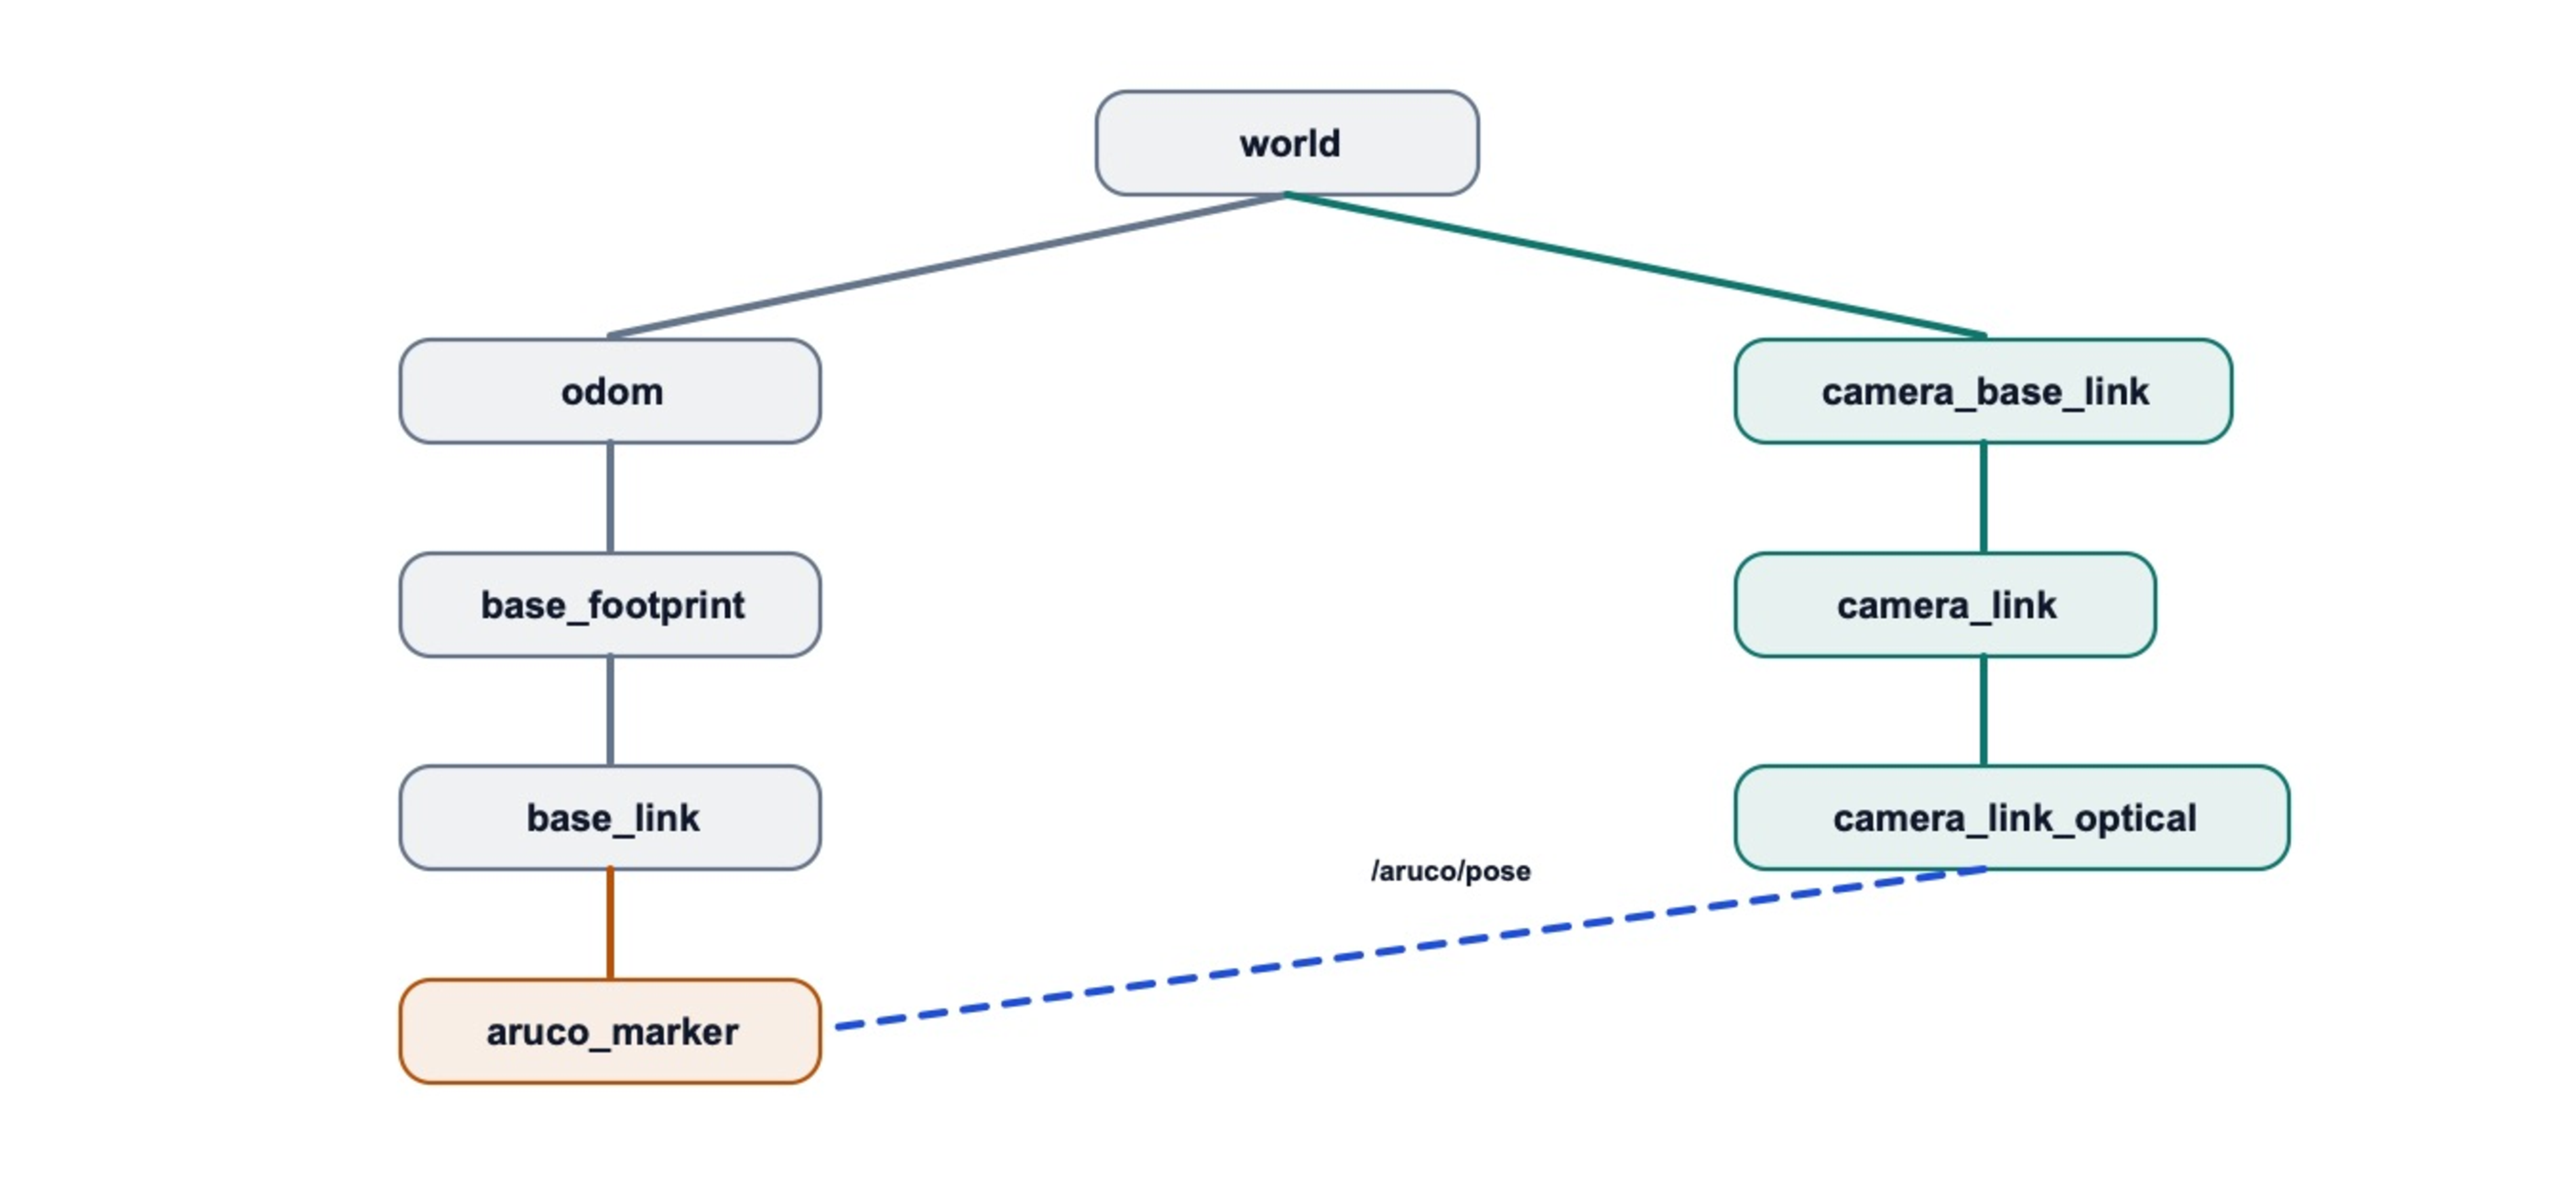
\includegraphics[width=\textwidth]{figures/diagrams/ros2_ecosystem_graph/tf2_frames_graph.pdf}
\caption{Marcos de referencia empleados en el framework. Se muestran el frame
global \texttt{world} \(\{w\}\), la referencia plana del robot
\texttt{base\_footprint} \(\{bf\}\), el torso \texttt{base\_link}
\(\{bl\}\), el frame del marcador ArUco \(\{a\}\) y la cadena de la cámara
hasta \texttt{camera\_link\_optical} \(\{c\}\). La salida publicada en
\texttt{/aruco/pose} queda expresada en ese frame óptico, de modo que esta
cadena geométrica es la base de la comparación entre pose estimada y ground
truth.}
\label{fig:theory_frames_overview}
\end{figure}

La distinción entre \texttt{base\_footprint} y \texttt{base\_link} es
especialmente útil porque parte de la reconstrucción del ground truth y de la
odometría se organiza respecto de una referencia desacoplada del balanceo
instantáneo del cuerpo. \texttt{base\_link} inclina y sube con el oleaje
sintético; \texttt{base\_footprint} preserva una referencia más ligada al plano
de apoyo. El frame del ArUco, a su vez, introduce el offset rígido del montaje,
y el frame de cámara permite expresar en un mismo sistema la observación visual
y la referencia reconstruida.

La misma lógica de marcos organiza la comparación entre estimación y ground
truth. Con esta notación, la pose observada del patrón puede escribirse como

\begin{equation}
{}^{c}\!T_a(t) =
{}^{c}\!T_w(t)\,{}^{w}\!T_{bf}(t)\,{}^{bf}\!T_{bl}(t)\,{}^{bl}\!T_a.
\label{eq:camera_marker_chain}
\end{equation}

Esta expresión resume dos ideas que reaparecen a lo largo de todo el trabajo.
Por un lado, la pose del marcador en cámara no depende sólo de la imagen, sino
de una cadena de transformaciones físicas entre mundo, robot, marcador y
sensor. Por otro lado, esa misma cadena permite reconstruir una referencia
comparable contra la cual medir el estimador visual: \({}^{w}\!T_{bf}\) fija la
pose global del robot, \({}^{bf}\!T_{bl}\) concentra la postura efectiva del
torso y \({}^{bl}\!T_a\) representa el montaje rígido del marcador. Para una
cámara fija, \({}^{c}\!T_w\) permanece constante; para una cámara montada sobre
el dron, ese término también varía en el tiempo. En ambos casos, el problema
de percepción se apoya en la misma organización geométrica.

\subsection{Marcadores fiduciales y estimación de pose}

Una vez que el movimiento existe y puede ser generado por el Go2, el problema se
traslada a la cámara: hay que recuperar, a partir de una imagen, la pose
relativa de un objeto plano cuya posición y orientación cambian continuamente.
Los marcadores fiduciales resultan apropiados para este escenario porque
introducen una geometría conocida y una identidad visual controlada dentro de
la escena. En particular, los marcadores ArUco combinan dos propiedades útiles
a la vez: un contorno cuadrado que permite localizar con precisión las esquinas
del patrón y un código binario interno que permite identificar de forma robusta
qué marcador está siendo observado \citep{GarridoJurado2014}. Esa combinación
vuelve al marcador simultáneamente detectable y geométricamente utilizable. La
robustez no depende solo de la segmentación del borde negro exterior, sino
también del diseño del diccionario: si los identificadores válidos están
suficientemente separados en distancia de Hamming, errores locales de lectura
producidos por ruido, desenfoque u oclusión parcial tienen menor probabilidad
de convertir un marcador en otro marcador válido.

Desde el punto de vista del pipeline, la detección del marcador es solo la
primera mitad del problema. La segunda consiste en estimar la transformación
rígida entre el patrón y la cámara a partir de correspondencias entre puntos
conocidos del marcador y sus proyecciones en la imagen. Ese es, precisamente,
el rol de \texttt{solvePnP}: resolver una instancia del problema
Perspective-\(n\)-Point usando la calibración intrínseca de la cámara y las
esquinas detectadas del marcador \citep{opencv_calib3d}. En otras palabras, el
detector no se limita a responder ``hay un ArUco''; produce una hipótesis
métrica sobre dónde está y cómo está orientado ese patrón respecto del sensor.

\begin{figure}[H]
\centering

\includegraphics[width=0.28\textwidth]{figures/images/aruco_id0_dict_6x6_250.png}
\caption{Marcador ArUco utilizado en el proyecto, correspondiente al identificador
\(0\) del diccionario \texttt{DICT\_6X6\_250}. Este es el patrón que se monta
sobre el Go2 y cuya pose se estima en tiempo real desde las cámaras simuladas.}
\label{fig:aruco_marker_id0}
\end{figure}

Si el lado del marcador es \(L\), sus cuatro vértices pueden definirse en el
frame del objeto como un conjunto coplanar de puntos conocidos:

\begin{equation}
P_1 = \left[-\frac{L}{2}, \frac{L}{2}, 0\right]^\top,\;
P_2 = \left[\frac{L}{2}, \frac{L}{2}, 0\right]^\top,\;
P_3 = \left[\frac{L}{2}, -\frac{L}{2}, 0\right]^\top,\;
P_4 = \left[-\frac{L}{2}, -\frac{L}{2}, 0\right]^\top.
\label{eq:marker_corners}
\end{equation}

La detección visual aporta las proyecciones bidimensionales
\(p_i = [u_i \;\; v_i \;\; 1]^\top\) de esos puntos en la imagen. La
consistencia entre el orden de los vértices observados y el orden de los
vértices del modelo es crucial, porque toda la estimación de pose depende de que
las correspondencias 2D--3D sean geométricamente correctas.

\figureplaceholder{fig:camera_marker_geometry}{Figura pendiente del modelo
geométrico cámara--marcador. Sería conveniente mostrar el frame óptico de la
cámara, el plano del marcador, sus cuatro vértices, el vector normal del patrón
y los rayos proyectivos que conectan las esquinas del objeto con el plano de la
imagen.}{Esquema pendiente de la proyección perspectiva de un marcador plano
observado por una cámara calibrada. Una figura de este tipo facilitaría la
lectura del modelo pinhole, de la homografía planar y del problema PnP.}

La relación entre los puntos tridimensionales del marcador y su proyección en la
imagen se describe mediante el modelo pinhole de cámara. Para cada punto
\(P_i = [X_i \;\; Y_i \;\; Z_i \;\; 1]^\top\), se cumple

\begin{equation}
s_i
\begin{bmatrix}
u_i \\
v_i \\
1
\end{bmatrix}
=
K
\begin{bmatrix}
R & t
\end{bmatrix}
\begin{bmatrix}
X_i \\
Y_i \\
Z_i \\
1
\end{bmatrix},
\label{eq:pinhole_projection}
\end{equation}

donde \(K\) es la matriz de parámetros intrínsecos

\begin{equation}
K =
\begin{bmatrix}
f_x & 0 & c_x \\
0 & f_y & c_y \\
0 & 0 & 1
\end{bmatrix},
\label{eq:camera_intrinsics}
\end{equation}

y \((R,t)\) representa la transformación rígida entre el frame del marcador y el
frame óptico de la cámara. Esta ecuación deja en evidencia una dependencia
fundamental del sistema: para estimar pose no alcanza con detectar el patrón; es
necesario conocer también la calibración intrínseca de la cámara y el tamaño
físico del marcador. Si la calibración es imprecisa, el error no aparece sólo en
la distancia estimada al marcador: también sesga la orientación recuperada,
porque ambos componentes se ajustan simultáneamente para explicar la misma
proyección 2D.

En el caso particular de un marcador plano, la geometría admite además una
formulación equivalente mediante homografía. Si todos los puntos del objeto
satisfacen \(Z_i = 0\), entonces la proyección se reduce a

\begin{equation}
s_i\,p_i = H
\begin{bmatrix}
X_i \\
Y_i \\
1
\end{bmatrix},
\label{eq:planar_homography}
\end{equation}

donde la homografía \(H\) puede descomponerse como

\begin{equation}
H = K
\begin{bmatrix}
r_1 & r_2 & t
\end{bmatrix},
\label{eq:homography_decomposition}
\end{equation}

siendo \(r_1\) y \(r_2\) las dos primeras columnas de la matriz de rotación
\(R\). Esta expresión muestra que un marcador plano no sólo aporta cuatro
correspondencias puntuales, sino una transformación proyectiva completa entre su
plano y la imagen. También explica por qué la estimación de pose con blancos
planares puede volverse ambigua o numéricamente delicada en configuraciones poco
favorables, por ejemplo cuando el patrón se observa casi frontalmente y el ruido
de esquina compite con una proyección muy poco deformada \citep{Schweighofer2006}.

La recuperación de \((R,t)\) puede formularse entonces como un problema de
Perspective-\(n\)-Point. En términos generales, se busca la transformación que
minimiza el error de reproyección entre los puntos observados y los puntos
predichos por el modelo:

\begin{equation}
(\hat{R},\hat{t}) =
\arg\min_{R,t}
\sum_{i=1}^{4}
\left\|
p_i - \pi\!\left(K(RP_i + t)\right)
\right\|_2^2,
\label{eq:pnp_optimization}
\end{equation}

donde \(\pi(\cdot)\) denota la proyección perspectiva en coordenadas de imagen.
Entre las soluciones eficientes para este problema se encuentra EPnP, que
permite estimar la pose a partir de correspondencias 2D--3D con costo lineal en
la cantidad de puntos \citep{Lepetit2009}. En el caso de un marcador cuadrado,
el número de puntos es pequeño, pero la formulación sigue siendo conceptualmente
la misma: a partir de cuatro esquinas coplanares y calibración conocida, se
recupera la pose del marcador respecto de la cámara. En la práctica, el objetivo
no es únicamente hallar una solución geométricamente válida, sino encontrar la
que minimiza de la manera más consistente el error inducido por ruido,
cuantización de píxeles y distorsión residual. Por eso, el error de
reproyección funciona como criterio natural para comparar hipótesis de pose.

Si se linealiza la proyección alrededor de una solución nominal
\((R_0,t_0)\), pequeñas perturbaciones en la imagen y en la pose quedan
relacionadas aproximadamente por un Jacobiano de sensibilidad \(J_\pi\):

\begin{equation}
\delta p \approx J_\pi\,\delta \xi,
\label{eq:projection_jacobian_linearization}
\end{equation}

donde \(\delta \xi\) representa una perturbación infinitesimal de la pose en el
espacio tangente de \(SE(3)\). Esta linealización ayuda a interpretar un hecho
empírico importante: cuanto más pequeñas aparecen las esquinas del marcador o
cuanto más cercana está la observación a una configuración proyectiva degenerada,
mayor es la sensibilidad de la pose estimada frente a pequeños errores de
localización.

Esta geometría proyectiva explica, además, por qué el recorte a roll, pitch y
heave es tan relevante en este problema. Si el marcador está fijado al torso del
robot, roll y pitch se reflejan principalmente en la parte rotacional de
\((R,t)\), mientras que heave altera la distancia relativa y, por lo tanto, la
escala aparente del patrón en la imagen. En otras palabras, el movimiento que
escogimos modelar no es solo una abstracción mecánica; es exactamente el
movimiento que el estimador visual tiene que reconstruir.



\section{Metodología}

En este trabajo organizamos la metodología en dos etapas complementarias. La
primera corresponde a la simulación, donde construimos un entorno controlado y
reproducible para modelar el movimiento de una plataforma marina, observarla
con distintas fuentes de imagen y evaluar la estimación visual contra un ground
truth conocido. La segunda corresponde al laboratorio, donde trasladamos parte
de esa lógica al robot real para analizar qué ocurre al pasar de un entorno
idealizado a uno físico y hasta qué punto el movimiento propuesto en simulación
guarda relación con el comportamiento observado en el Go2.

\subsection{Metodología en simulación}

La simulación fue el primer entorno de validación del framework porque nos
permitió controlar la escena, repetir corridas bajo condiciones comparables y
registrar todas las señales relevantes del sistema. En esta etapa el problema
se organizó como un pipeline de cuatro pasos: generación del movimiento
marino, materialización de ese movimiento en el Go2, observación visual del
marcador y evaluación offline contra una referencia reconstruible. Sobre la
base conceptual introducida en el Capítulo~\ref{mt}, aquí nos concentramos en
cómo se implementó cada una de esas etapas y con qué configuración se ejecutó
la campaña experimental.

Además de servir como entorno de desarrollo, la simulación funcionó como un
banco de pruebas metodológico. Cada corrida se registró como un rosbag de un
minuto, lo que permitió volver sobre una misma secuencia para analizarla varias
veces sin repetir la ejecución completa. Dentro de esa estructura, la cámara
fija se utilizó como caso base y el \texttt{sjtu\_drone} como extensión más
exigente del mismo pipeline.

\subsubsection{Generación del movimiento marino}

En simulación no modelamos un casco marino completo ni resolvemos su dinámica
hidrodinámica detallada. Operativamente, el nodo
\texttt{marine\_platform\_simulator} sintetiza directamente sobre el Go2 una
consigna postural del torso en el tópico correspondiente
(Tabla~\ref{tab:ros_interfaces_sim}) y trata al robot como plataforma
instrumentada para el marcador ArUco. La implementación se concentra, entonces,
en la parte del problema que realmente interesa medir en este trabajo: cómo cambia
la apariencia del marcador cuando la plataforma se inclina y se desplaza
verticalmente.

El nodo opera con una frecuencia de publicación de \mbox{20 Hz} y toma como
referencia el tiempo transcurrido desde su inicialización. La configuración de
referencia del repositorio —la misma que adoptamos como base metodológica—
queda resumida en la Tabla~\ref{tab:method_marine_params}, donde
cada fila asocia un hiperparámetro con su valor y su función en la señal
sintetizada. Se eligió ese conjunto porque es el que efectivamente se usa para
correr la simulación completa del repositorio y, por tanto, el mejor documentado
y el más simple de reproducir. En la práctica, estos parámetros controlan
cuatro aspectos distintos del movimiento: su velocidad temporal, su amplitud
máxima, el desacople relativo entre ejes y la suavidad de la señal publicada.

\begin{table}[H]
\centering
\caption{Parámetros de referencia del simulador marino y función metodológica de
cada uno.}
\label{tab:method_marine_params}
\begin{tabular}{lll}
\toprule
Parámetro & Valor base & Función en la señal \\
\midrule
\texttt{rate\_hz} & \(20{,}0\) & Frecuencia de publicación del nodo \\
\texttt{wave\_frequency} & \(0{,}1\) Hz & Escala temporal del oleaje sintetizado \\
\texttt{max\_roll\_deg} & \(15{,}0^\circ\) & Amplitud máxima de roll \\
\texttt{max\_pitch\_deg} & \(10{,}0^\circ\) & Amplitud máxima de pitch \\
\texttt{max\_heave\_m} & \(0{,}10\) m & Amplitud máxima de heave \\
\texttt{phase\_offset\_pitch} & \(1{,}0\) & Desacople temporal de pitch \\
\texttt{phase\_offset\_heave} & \(1{,}5\) & Desacople temporal de heave \\
\texttt{smoothing\_factor} & \(0{,}95\) & Suavizado exponencial de la consigna \\
\bottomrule
\end{tabular}
\end{table}

La Tabla~\ref{tab:method_marine_params} cumple un rol metodológico importante:
permite leer cada hiperparámetro no como una opción aislada del código, sino
como una decisión que modifica la dificultad del escenario visual. Aumentar la
frecuencia acelera la variación temporal del marcador; aumentar las amplitudes
agranda las excursiones angulares y verticales; modificar los desfases cambia
la relación temporal entre ejes; y variar el suavizado altera cuán brusca o
cuán continua resulta la señal final.

Las interfaces ROS~2 usadas en simulación y en la evaluación \textit{offline}
se listan de forma canónica en la Tabla~\ref{tab:ros_interfaces_sim}; las del
montaje en laboratorio, en la Tabla~\ref{tab:ros_interfaces_lab}. En el resto
del documento se alude a esas señales por su \emph{rol} en prosa y se remite a
esas tablas, en lugar de repetir los identificadores completos en cada párrafo.

\begin{table}[H]
\centering
\footnotesize
\caption{Tópicos ROS~2 principales en simulación y evaluación \textit{offline}
(roles y literales).}
\label{tab:ros_interfaces_sim}
\begin{adjustbox}{max width=\textwidth}
\begin{tabular}{p{0.30\textwidth}p{0.38\textwidth}p{0.28\textwidth}}
\toprule
Rol en el pipeline & Tópico & Tipo de mensaje \\
\midrule
Consigna postural del torso & \path{/body_pose} & \texttt{geometry\_msgs/Pose} \\
Depuración del simulador marino (roll, pitch, heave) & \path{/marine_platform/debug_state} & \texttt{geometry\_msgs/Vector3} \\
Comandos en modo manual & \path{/marine_platform/manual_cmd} & \texttt{geometry\_msgs/Vector3} \\
Odometría & \path{/odom} & \texttt{nav\_msgs/Odometry} \\
IMU & \path{/imu/data} & \texttt{sensor\_msgs/Imu} \\
Pose base--footprint & \path{/base_to_footprint_pose} & \texttt{geometry\_msgs/PoseStamped} \\
Pose estimada del ArUco & \path{/aruco/pose} & \texttt{geometry\_msgs/PoseStamped} \\
Detección del ArUco & \path{/aruco/detection} & mensajes del nodo \texttt{aruco\_detector} \\
Imagen de depuración & \path{/aruco/debug_image} & \texttt{sensor\_msgs/Image} \\
Imagen cámara fija & \path{/fixed_camera/camera/image_raw} & \texttt{sensor\_msgs/Image} \\
Información de cámara fija & \path{/fixed_camera/camera/camera_info} & \texttt{sensor\_msgs/CameraInfo} \\
\bottomrule
\end{tabular}
\end{adjustbox}
\end{table}

\begin{table}[H]
\centering
\footnotesize
\caption{Tópicos ROS~2 adicionales o centrales en el laboratorio (comando y
estado del Go2 real).}
\label{tab:ros_interfaces_lab}
\begin{adjustbox}{max width=\textwidth}
\begin{tabular}{p{0.30\textwidth}p{0.38\textwidth}p{0.28\textwidth}}
\toprule
Rol en el pipeline & Tópico & Tipo de mensaje \\
\midrule
Depuración del simulador marino (modo real) & \path{/marine_platform/debug_state} & \texttt{geometry\_msgs/Vector3} \\
Peticiones a la API Sport Mode & \path{/api/sport/request} & mensajes Unitree (SDK2) \\
Estado deportivo del robot & \path{/sportmodestate} & mensajes Unitree \\
Estado de bajo nivel & \path{/lowstate} & mensajes Unitree \\
Odometría (contraste) & \path{/utlidar/robot_odom} & \texttt{nav\_msgs/Odometry} \\
Imagen del ojo izquierdo (estéreo) & \path{/stereo_camera/image_raw} & \texttt{sensor\_msgs/Image} \\
Calibración del estéreo & \path{/stereo_camera/camera_info} & \texttt{sensor\_msgs/CameraInfo} \\
\bottomrule
\end{tabular}
\end{adjustbox}
\end{table}

El patrón de referencia del trabajo es el sinusoidal. Si denotamos por \(A_r\),
\(A_p\) y \(A_h\) las amplitudes máximas de roll, pitch y heave, y por
\(\omega = 2 \pi f\) la pulsación angular asociada a la frecuencia base
\(f\), el nodo implementa:

\begin{equation}
r(t) = A_r \sin(\omega t),
\end{equation}

\begin{equation}
p(t) = A_p \sin(\omega \kappa_p t + \pi/3),
\end{equation}

\begin{equation}
h(t) = A_h \sin(\omega \kappa_h t),
\end{equation}

donde \(\kappa_p\) y \(\kappa_h\) corresponden a los parámetros
\texttt{phase\_offset\_pitch} y \texttt{phase\_offset\_heave}. En la
configuración de referencia, \(\kappa_p = 1{,}0\) y \(\kappa_h = 1{,}5\). Esto
hace que roll y pitch evolucionen en escalas temporales similares, mientras que
heave introduce una oscilación algo más rápida. A su vez, el desfase fijo de
\(\pi/3\) en pitch evita que las tres componentes alcancen sus extremos al
mismo tiempo. Incluso en esta versión simple, el movimiento resultante no es
una oscilación rígidamente sincronizada, sino una combinación periódica más
interesante para observar cómo responde el estimador visual.

Adoptamos el patrón sinusoidal como referencia metodológica por tres razones.
Primero, cada hiperparámetro tiene un efecto fácilmente interpretable sobre la
señal. Segundo, la excitación es altamente repetible, lo que permite comparar
rosbags distintos sin introducir ambigüedad sobre la entrada del sistema.
Tercero, la relación entre frecuencia, amplitud y fase se reconoce con claridad
tanto en las señales del robot como en la imagen del marcador.

\begin{figure}[H]
\centering
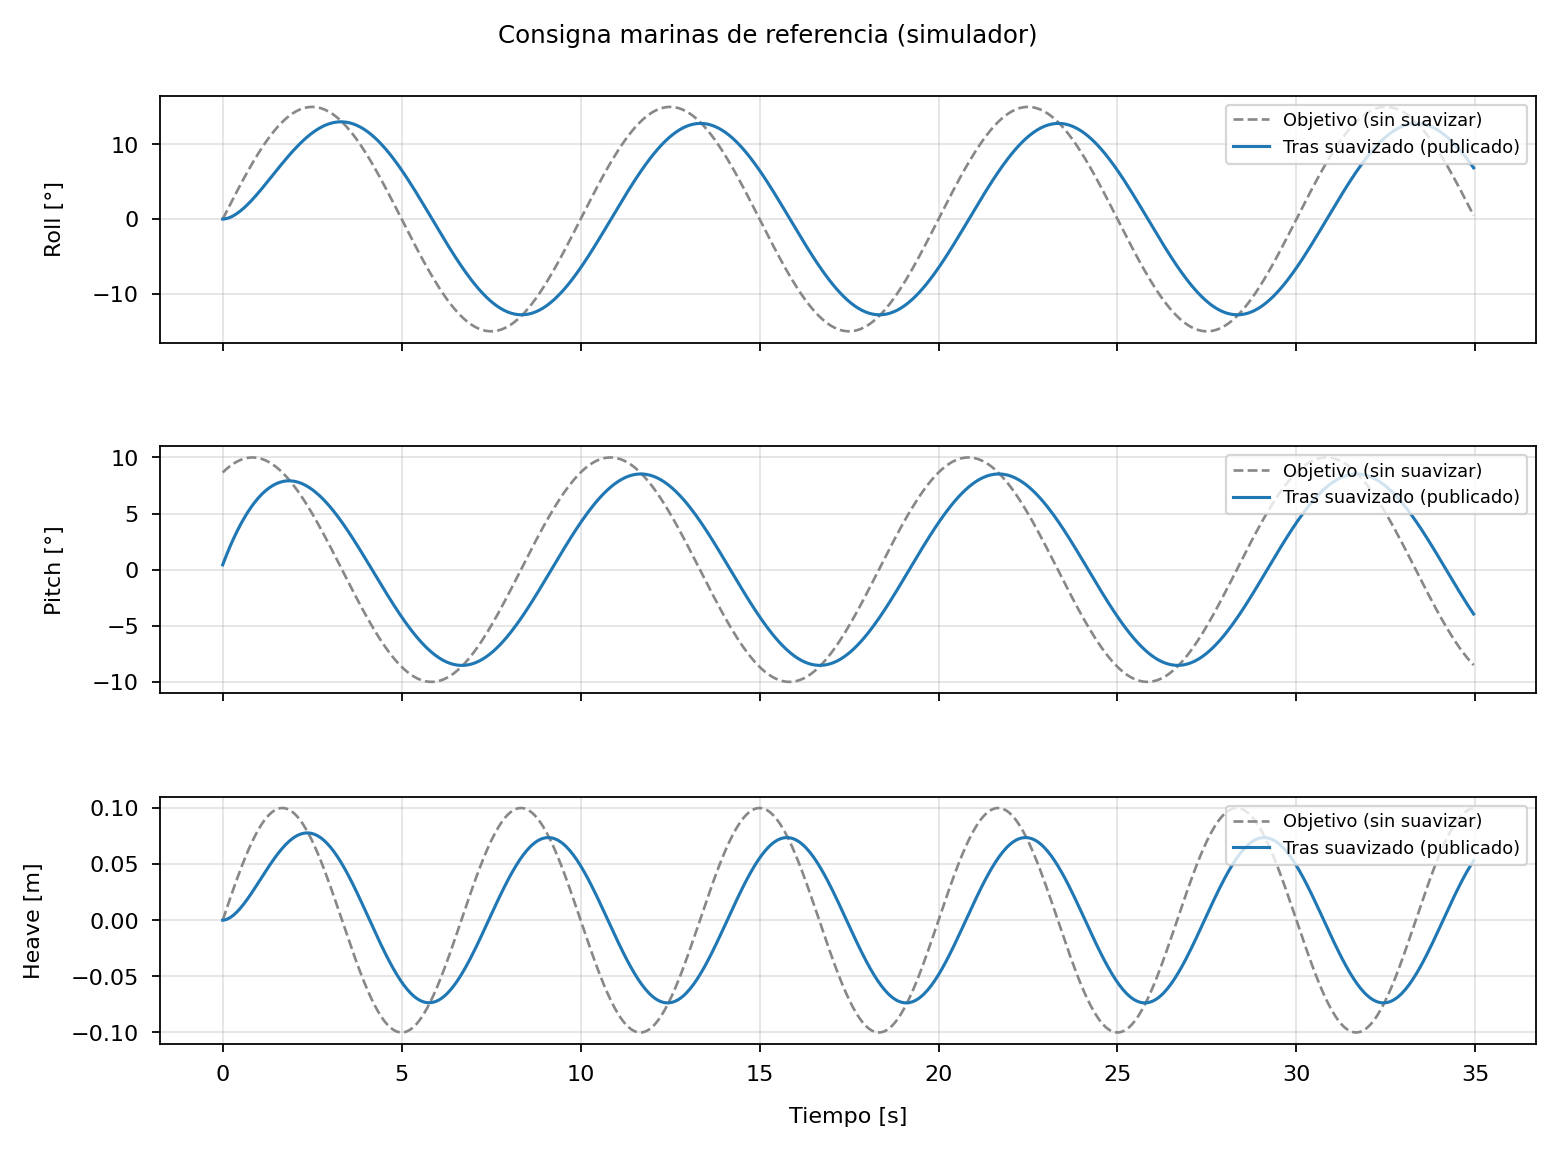
\includegraphics[width=\textwidth]{figures/images/fig_method_motion_components.png}
\caption{Componentes temporales de roll, pitch y heave en modo
\texttt{sinusoidal} con los valores por defecto del nodo
\texttt{marine\_platform\_simulator} (\(f=0{,}1\) Hz,
\(A_r=\pm 15^\circ\), \(A_p=\pm 10^\circ\), \(A_h=\pm 0{,}1\) m,
\(\kappa_p=1\), \(\kappa_h=1{,}5\), desfase fijo \(\pi/3\) en pitch).
La línea punteada es la consigna objetivo antes del filtro; la continua es la
señal suavizada (\(\alpha=0{,}95\)) que se publica como consigna postural y en
el tópico de depuración del simulador marino (Tabla~\ref{tab:ros_interfaces_sim}).}
\label{fig:method_motion_components}
\end{figure}

El nodo también ofrece un patrón \texttt{irregular}, construido como suma de
varias componentes sinusoidales por eje. Ese modo se utilizó durante el
desarrollo para exploración y depuración, porque rompe la periodicidad estricta
del caso simple y expone al detector a perturbaciones menos regulares. Sin
embargo, no lo tomamos como caso principal de la evaluación porque no fue calibrado
como un modelo físico de mar y resultaba menos conveniente como base
reproducible para comparar estimación y ground truth. Por esa razón, el patrón
sinusoidal quedó como referencia metodológica del trabajo, mientras que el
irregular se mantuvo como variante complementaria de ensayo.

En términos prácticos, la diferencia entre ambos modos puede resumirse así: el
patrón sinusoidal concentra la variación de cada eje en una componente dominante
y vuelve más transparente la relación entre entrada y respuesta; el patrón
\texttt{irregular}, en cambio, superpone oscilaciones con distintas escalas
temporales y genera trayectorias menos previsibles. Esta segunda opción es útil
para tensionar el detector y explorar la robustez del pipeline, pero no resulta
la mejor base cuando se quiere explicar el sistema con claridad o comparar una
configuración con otra de manera controlada.

\begin{figure}[H]
\centering
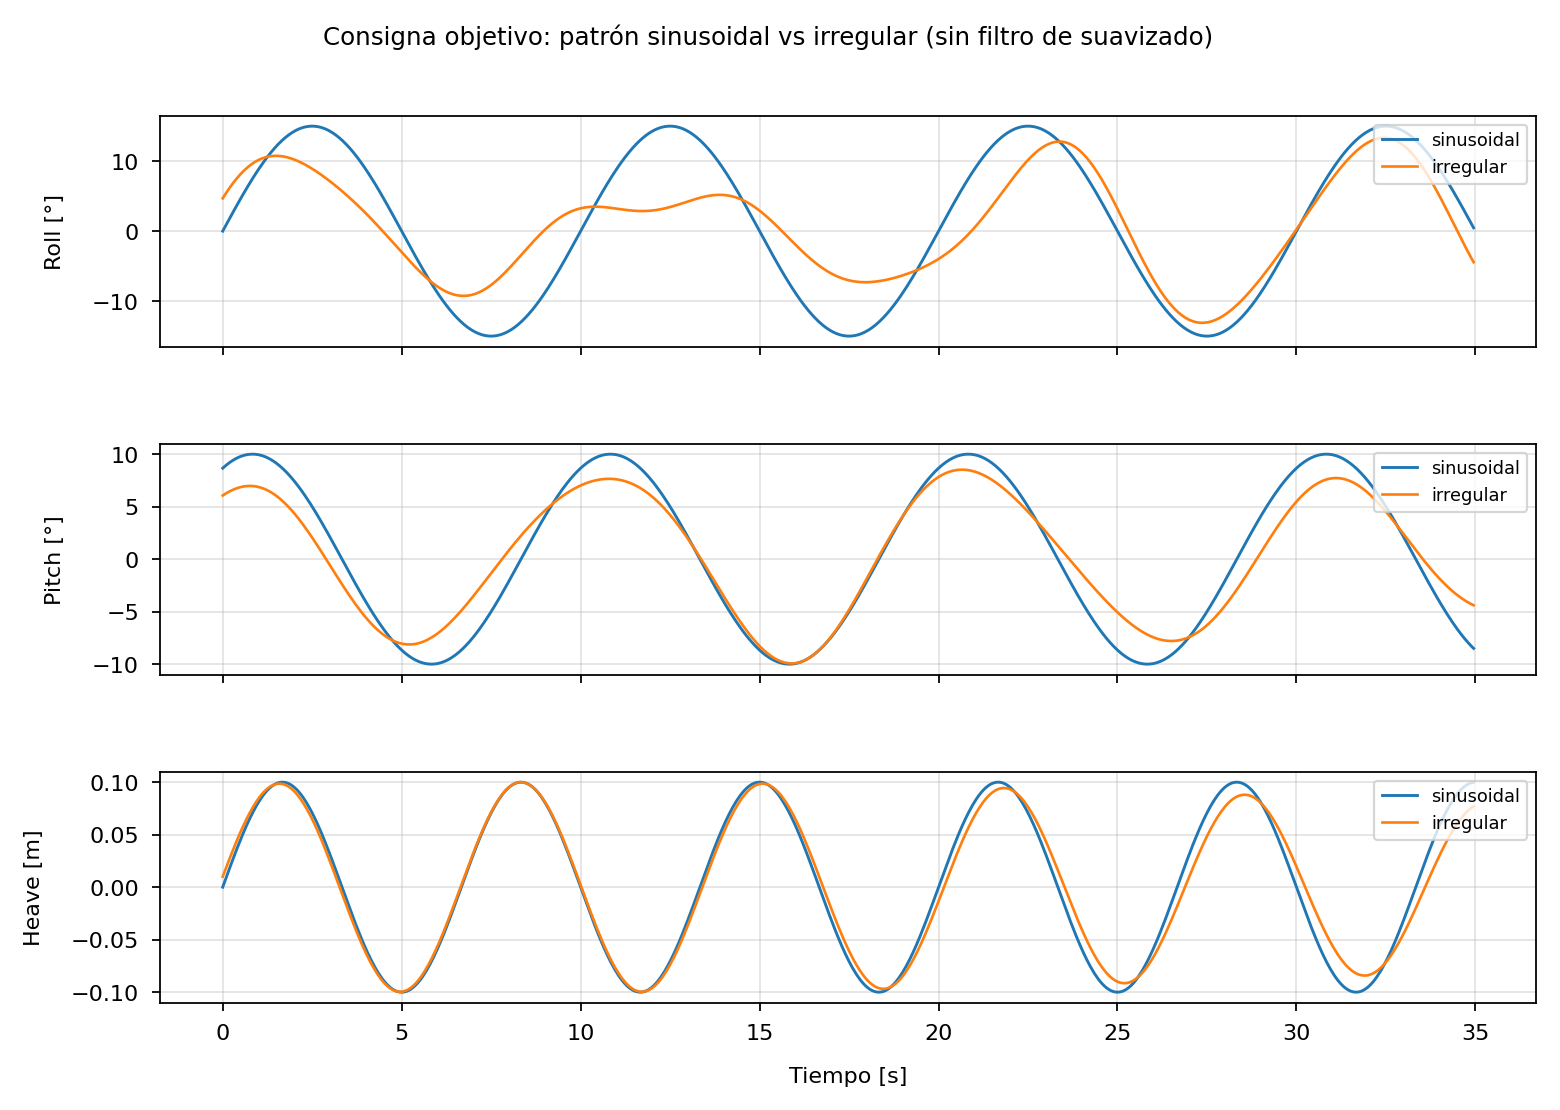
\includegraphics[width=\textwidth]{figures/images/fig_method_wave_patterns.png}
\caption{Comparación entre los patrones \texttt{sinusoidal} e
\texttt{irregular} implementados en \texttt{marine\_platform\_simulator} para
los mismos límites de amplitud y frecuencia base. El modo sinusoidal concentra
cada eje en una componente periódica simple; el modo irregular superpone
varias sinusoides con distintas frecuencias relativas, generando trayectorias
menos previsibles. La figura muestra la consigna \emph{objetivo} antes del
filtro de suavizado. Se adoptó el patrón sinusoidal como referencia metodológica
porque resulta más interpretable y reproducible para comparar estimación y
ground truth.}
\label{fig:method_wave_patterns}
\end{figure}

Una vez calculada la señal objetivo para cada eje, el nodo no la publica de
forma directa. Antes aplica un suavizado exponencial, implementado como un
filtro pasa-bajos de primer orden. Si \(\alpha\) denota el parámetro
\texttt{smoothing\_factor} y \(x_k\) el valor objetivo en el instante discreto
\(k\), la señal publicada \(\tilde{x}_k\) se obtiene mediante

\begin{equation}
\tilde{x}_k = \alpha \tilde{x}_{k-1} + (1-\alpha) x_k.
\end{equation}

El mismo esquema se usa para roll, pitch y heave. En la configuración base,
\(\alpha = 0{,}95\), de modo que la salida conserva una memoria fuerte del
estado previo y amortigua cambios abruptos entre iteraciones consecutivas. Esto
ayuda a evitar transiciones poco plausibles en Gazebo y reduce movimientos
demasiado bruscos que podrían introducir artefactos innecesarios en la
evaluación visual. Metodológicamente, este parámetro fue importante porque
funciona como puente entre una señal objetivo ideal y una consigna más cercana
a un movimiento físicamente ejecutable por el robot.

Luego del suavizado, el nodo construye un mensaje \texttt{Pose}. La posición se
fija como \((0, 0, \tilde{h}_k)\), de manera que el único desplazamiento lineal
es la componente vertical. La orientación se representa con roll y pitch
suavizados, mientras que yaw se mantiene en cero. Como ROS2 publica
orientaciones en cuaterniones, el nodo convierte primero los ángulos a radianes
y calcula después el cuaternión correspondiente antes de emitir la consigna
postural del torso. En paralelo, publica un \texttt{Vector3} en el tópico de
depuración del simulador marino con los valores suavizados de roll,
pitch y heave (Tabla~\ref{tab:ros_interfaces_sim}), lo que facilita la
inspección de la corrida y el contraste posterior con la evaluación offline.

El simulador también incorpora un modo manual. Cuando
\texttt{enable\_manual=true}, deja de sintetizar ondas automáticamente y pasa a
consumir comandos en el tópico de modo manual (Tabla~\ref{tab:ros_interfaces_sim}). Un
segundo nodo, \texttt{marine\_manual\_control}, permite generar esas consignas
desde teclado con incrementos discretos en roll, pitch y heave, además de
aplicar saturaciones de seguridad y recuperar una posición neutral. Este modo
no fue la base de las corridas experimentales, pero sí resultó valioso para
verificar poses aisladas, revisar la coherencia geométrica de la escena y
diagnosticar problemas antes de pasar a secuencias continuas de oleaje. En ese
sentido, cumplió un rol de apoyo en el desarrollo: permitió inspeccionar el
pipeline en estados controlados antes de exigirle seguimiento continuo sobre
secuencias periódicas de un minuto.

\figureplaceholder
  {fig:method_marine_simulator}
  {Esquema del nodo \texttt{marine\_platform\_simulator}: parámetros de oleaje,
  publicación de la consigna postural, modo manual y relación con el torso del
  Go2 en Gazebo.}
  {Arquitectura del simulador marino utilizado para generar roll, pitch y heave
  sobre el cuerpo del Go2.}

\subsubsection{Control postural del Go2 en simulación}

El nodo \texttt{marine\_platform\_simulator} no mueve directamente un objeto
externo en Gazebo, sino que publica una pose deseada del cuerpo del Go2 en el
tópico de consigna postural. Esa consigna contiene \(x=y=0\), \texttt{yaw}=0, una
altura variable asociada a heave y una orientación dada por roll y pitch. El
objetivo de este diseño es que la ``plataforma marina'' no sea una malla rígida
desacoplada del robot, sino la propia postura del cuadrúpedo.

Durante el bringup del Go2 en simulación, el stack de control del robot consume
esa pose deseada del torso y la traduce en una nueva configuración articular.
Desde un punto de vista funcional, el proceso puede leerse de la siguiente
manera: a partir de una postura nominal, el controlador reubica las patas para
que el cuerpo adopte la altura y la inclinación solicitadas. El efecto buscado
no se logra desplazando rígidamente el \textit{base link} del robot, sino
reconfigurando la postura completa del cuadrúpedo de un modo consistente con su
cadena cinemática.

Esta decisión fue importante porque mantiene la coherencia entre la simulación
visual y el resto de las señales del sistema. El Go2 no solo se ve inclinado
desde la cámara, sino que además publica estados compatibles con esa postura,
como odometría, IMU y estimaciones de pose del cuerpo. En otras palabras, el
movimiento marino sintetizado no aparece únicamente como una animación del
modelo, sino como una secuencia reproducible de configuraciones del robot que
puede seguirse también desde sus variables internas.

Esa misma cadena de estado es la que luego se usa para construir el ground
truth del marcador. En la evaluación offline se reconstruye primero la pose del
tronco a partir de la odometría, la IMU y la pose base--footprint
(Tabla~\ref{tab:ros_interfaces_sim}); después se suma el offset fijo del ArUco
respecto del cuerpo del Go2 y se corrige el offset de \textit{spawn} del robot
en el mundo, fijado en \(0{,}40\) m sobre el eje \(x\) en la configuración de
referencia. De este modo, la pose verdadera del marcador no se toma como un
dato trivial del simulador, sino como una cantidad reconstruida de forma
consistente con el resto del pipeline.

\subsubsection{Estimación visual en simulación}

Como se discutió en el Capítulo~\ref{mt}, el framework contempla dos fuentes de
imagen complementarias. Operativamente, la primera es una cámara fija nadir,
ubicada sobre la plataforma y orientada hacia abajo. La segunda es la cámara
bottom del \texttt{sjtu\_drone}, que despega automáticamente y luego mantiene un
hover por encima del Go2. La Figura~\ref{fig:method_visual_setup} resume
visualmente ambos casos.

\begin{figure}[H]
\centering
\begin{subfigure}[t]{0.28\textwidth}
\centering
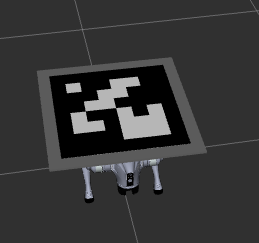
\includegraphics[width=\textwidth]{figures/setup/unitree-aruco.png}
\caption{Go2 con el marcador ArUco montado sobre el torso.}
\end{subfigure}
\hfill
\begin{subfigure}[t]{0.62\textwidth}
\centering
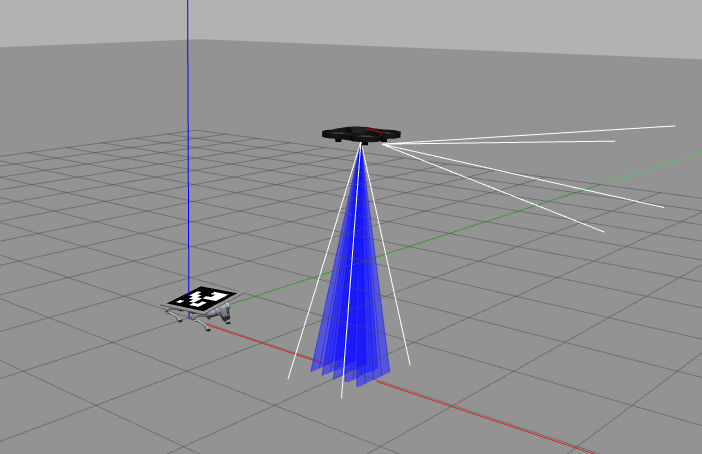
\includegraphics[width=\textwidth]{figures/setup/drone-unitree-aruco.png}
\caption{Escenario con el \texttt{sjtu\_drone} en hover sobre la plataforma.}
\end{subfigure}
\caption{Vistas del entorno simulado utilizadas en el framework. A la izquierda
se observa la plataforma instrumentada con el marcador; a la derecha, el caso
con cámara aérea, donde la percepción depende además de la pose del dron.}
\label{fig:method_visual_setup}
\end{figure}

La Figura~\ref{fig:method_frames_scene} complementa esa vista con una
superposición de ternas sobre la propia escena simulada. Así, los marcos
discutidos en el Capítulo~\ref{mt} dejan de aparecer como una cadena abstracta y
pueden leerse directamente sobre la relación espacial entre el dron, el Go2 y
el marcador.

\begin{figure}[H]
\centering
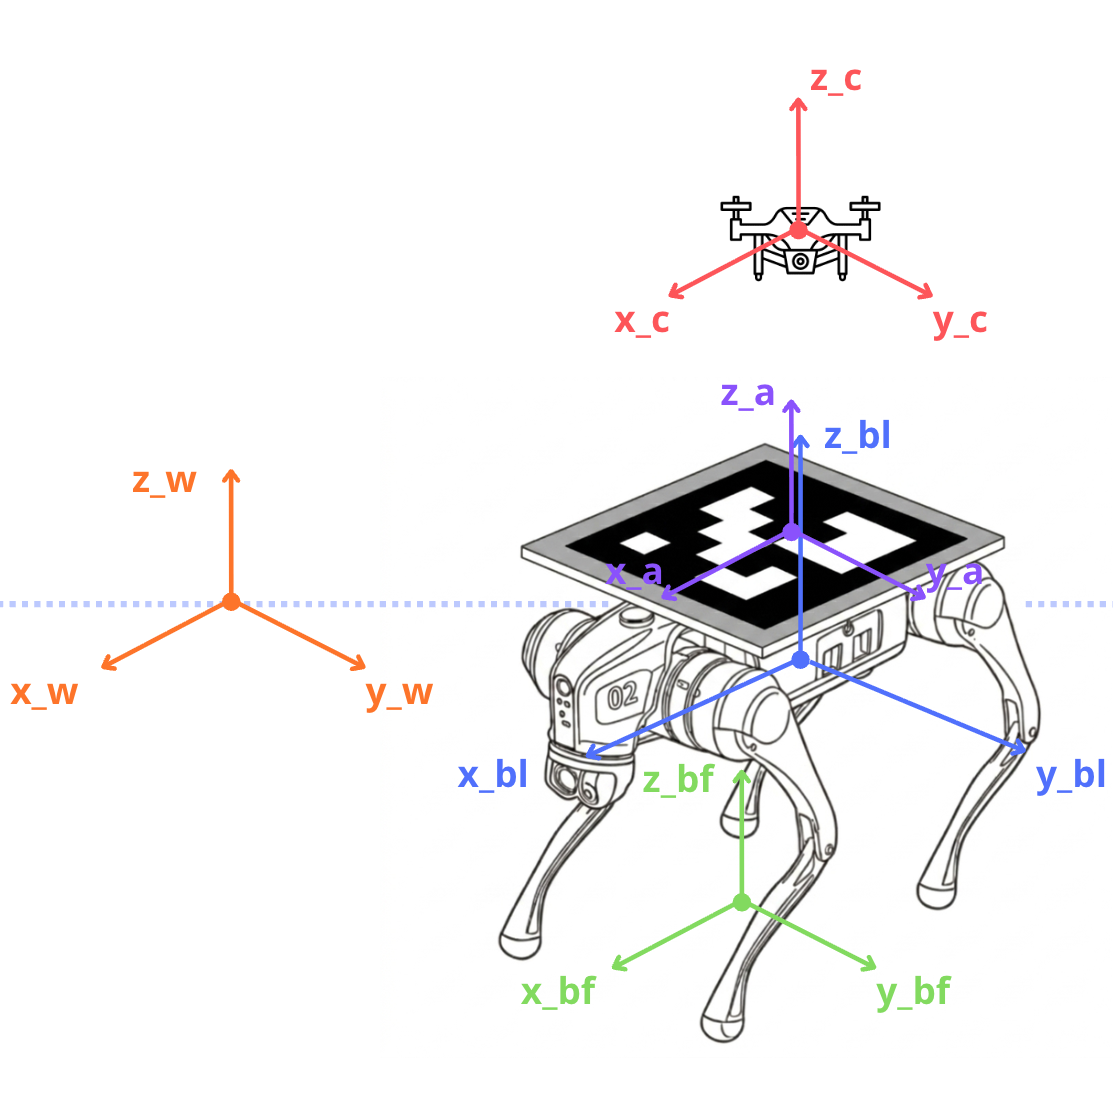
\includegraphics[width=0.62\textwidth]{figures/diagrams/ternas.png}
\caption{Vista esquemática del montaje con cámara aérea y superposición de las
ternas principales del pipeline geométrico. Se muestran el frame global
\texttt{world}, la referencia \texttt{base\_footprint}, el torso
\texttt{base\_link}, el frame del marcador ArUco y el frame de la cámara
embarcada en el dron. Esta imagen permite ubicar sobre la escena concreta las
referencias que después intervienen en la estimación visual y en la
reconstrucción del ground truth.}
\label{fig:method_frames_scene}
\end{figure}

En ambos casos la estimación visual se resolvió con un nodo
\texttt{aruco\_detector} dedicado. El detector consume la imagen RGB y la
calibración intrínseca de la cámara, busca el marcador del diccionario
\texttt{DICT\_6X6\_250} con identificador \(0\) y asume un lado de \(0{,}50\)
metros. Una vez detectadas las esquinas, OpenCV estima la pose relativa del
marcador respecto del frame óptico de la cámara mediante \texttt{solvePnP}. El
resultado se publica como \texttt{PoseStamped} en el tópico de pose del ArUco,
mientras que la detección y la imagen de depuración se publican en los canales
asociados (Tabla~\ref{tab:ros_interfaces_sim}) para inspección y depuración.
Durante la corrida, el detector trabaja solo con imagen e intrínsecos de
cámara: no usa conocimiento privilegiado del simulador, de la pose del robot ni
de la pose del dron. Un
ejemplo del frame anotado que produce el detector puede verse en la
Figura~\ref{fig:method_aruco_detection_frame}.

\begin{figure}[H]
\centering
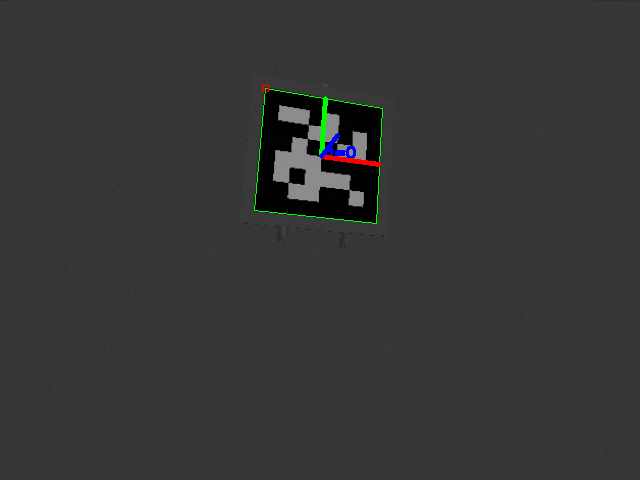
\includegraphics[width=0.68\textwidth]{figures/images/aruco_detection_frame.png}
\caption{Salida visual del detector ArUco durante una corrida de simulación. Se
observa el marcador \texttt{DICT\_6X6\_250} con identificador \(0\) sobre el
torso del Go2, junto con los ejes de pose estimada superpuestos en tiempo real.}
\label{fig:method_aruco_detection_frame}
\end{figure}

En el caso base, la cámara fija se modeló como un sensor estático en Gazebo con
una altura nominal de \(2{,}0\) m y con imagen e información de cámara en los
tópicos listados en la Tabla~\ref{tab:ros_interfaces_sim}. Su frame permanece rígido respecto
del mundo, de modo que toda la variabilidad de la secuencia proviene del
movimiento del Go2. En el caso del dron, por el contrario, la cámara deja de
ser un observador inmóvil. El \texttt{sjtu\_drone} se spawnea con un offset
horizontal respecto del robot, ejecuta el takeoff de forma automática y, tras
un retardo de tres segundos, conmuta a control por posición para mantener un
hover nominal en \((0{,}5,\ 0,\ 3{,}0)\) m. Esta organización permite pasar de
un escenario geométricamente más limpio a otro donde la percepción depende
además de la dinámica del vehículo aéreo.

\begin{figure}[H]
\centering
\begin{subfigure}[t]{0.49\textwidth}
\centering

\includegraphics[width=\linewidth]{figures/images/fig_sim_fixed_camera_raw.png}
\caption{Vista cruda desde la cámara fija nadir.}
\end{subfigure}
\hfill
\begin{subfigure}[t]{0.49\textwidth}
\centering
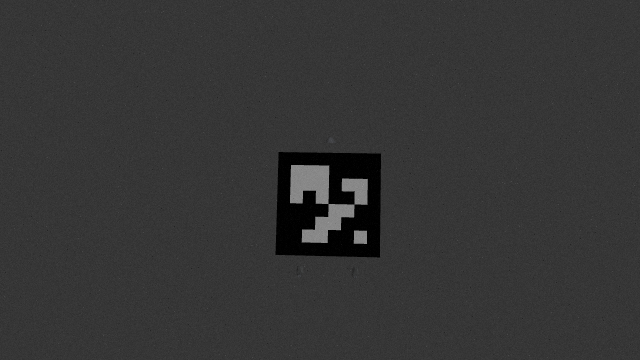
\includegraphics[width=\linewidth]{figures/images/fig_sim_sjtu_drone_raw.png}
\caption{Vista cruda desde la cámara bottom del \texttt{sjtu\_drone}.}
\end{subfigure}
\caption{Comparación entre las dos fuentes de imagen empleadas en simulación
para la estimación de pose del ArUco en tiempo real.}
\label{fig:method_camera_sources}
\end{figure}

\subsubsection{Registro y evaluación offline}

La etapa de simulación se cerró siempre con el registro de la corrida en un
rosbag de aproximadamente un minuto. Ese registro incluye, según el escenario,
la imagen de la cámara, su calibración, la pose estimada del ArUco, TF,
odometría, IMU y las señales necesarias para reconstruir después la pose
verdadera del marcador. De esta manera, cada sesión queda preservada como una
unidad de análisis que puede reprocesarse sin volver a ejecutar Gazebo.

La evaluación se separó deliberadamente de la percepción en tiempo real. Durante
la corrida, el detector procesa únicamente imagen e intrínsecos de cámara. La
comparación con el ground truth se hace después, a partir del rosbag, mediante
el script \texttt{evaluate\_realtime\_aruco.py}. En ese análisis offline se
reconstruye la pose del tronco del Go2 en el mundo usando las mismas señales de
estado listadas en la Tabla~\ref{tab:ros_interfaces_sim}; luego se suma el
offset fijo del marcador sobre el cuerpo del robot y se transforma esa pose al
frame de la cámara mediante las extrínsecas definidas en cada setup. En el caso
del dron, además, entra la pose del propio vehículo como parte de la cadena de
transformaciones. En otras palabras, el postproceso recompone la cadena
geométrica de la Ecuación~\ref{eq:camera_marker_chain} y de la
Figura~\ref{fig:theory_frames_overview}: a partir de la pose global del robot,
su postura efectiva y el montaje rígido del marcador, se obtiene una referencia
en frame cámara directamente comparable con la salida de \texttt{solvePnP}.

Esta separación entre estimación online y análisis offline resultó importante
por dos motivos. En primer lugar, evita contaminar la medición del desempeño
con información del simulador que no estaría disponible en una aplicación real.
En segundo lugar, permite revisar una misma secuencia con distintos criterios de
análisis sin modificar el detector ni repetir la simulación. Sobre esa base se
generan los CSV y los gráficos de error que luego alimentan el capítulo
experimental.

Con este pipeline ya estabilizado, la campaña final de simulación del capítulo
se organizó como un conjunto de corridas comparables bajo un único perfil
experimental, al que nos referiremos como configuración de referencia. Esa
campaña fijó una excitación sinusoidal común, mantuvo constante el offset de
spawn del Go2 \((world\_init\_x = 0{,}40,\ world\_init\_y = 0)\) y repitió el
mismo montaje visual en cuatro rosbags: un baseline con \texttt{fixed\_camera}
y tres repeticiones del escenario \texttt{sjtu\_drone}. La motivación de este
diseño fue separar con claridad dos preguntas. La primera, de carácter
metodológico, fue qué tan bien sigue el pipeline visual el movimiento sintético
cuando el sensor permanece fijo. La segunda, ya más cercana al objetivo final
del framework, fue cuánto se degrada esa estimación cuando la observación pasa a
depender también de una cámara aérea embarcada en el dron. Esta estructura de
campaña se retoma en el capítulo experimental y explica por qué la comparación
principal del capítulo no se plantea como una única corrida ejemplar, sino como
un baseline más tres repeticiones comparables del caso fuerte.

\figureplaceholder
  {fig:method_pipeline}
  {Pipeline completo desde Gazebo hasta la evaluación offline: simulador marino,
  fuente de imagen, detección ArUco, grabación en rosbag y comparación posterior
  contra ground truth.}
  {Pipeline implementado para estimar en tiempo real la pose del marcador y
  evaluarla luego contra el estado verdadero del simulador.}

\subsection{Metodología en laboratorio}

Una vez estabilizado el pipeline en simulación, trasladamos parte de la
metodología al laboratorio para estudiar el pasaje desde un entorno controlado
hacia uno físico. En esta segunda etapa el objetivo ya no fue disponer de un
ground truth perfecto como en Gazebo, sino verificar dos cuestiones más
concretas: primero, si el movimiento propuesto sobre el torso del Go2 puede
reproducirse de manera razonable en el robot real; y segundo, si ese movimiento
puede observarse visualmente mediante un marcador ArUco y una cámara mantenida
en posición aproximadamente fija. Este pasaje implicó cambios prácticos en el
montaje, en las condiciones de medición y en el tipo de comparación que podía
realizarse respecto de la simulación.

\subsubsection{Dificultades del pasaje de simulación a laboratorio}

El pasaje de simulación a laboratorio no consistió en trasladar sin cambios un
pipeline ya resuelto, sino en adaptar cada una de sus partes a un entorno donde
desaparecen varias de las idealizaciones de Gazebo. En simulación, la escena, la
calibración de cámara, el montaje del sensor y el estado del robot están
definidos por el modelo. En laboratorio, en cambio, esas mismas piezas deben
construirse y verificarse experimentalmente: la cámara requiere calibración
real, el marcador debe montarse físicamente sobre el robot, la posición del
sensor deja de ser perfectamente rígida y la comparación ya no puede apoyarse en
un ground truth exacto del sistema.

Desde el punto de vista metodológico, hubo tres adaptaciones importantes. La
primera afectó a la entrada del sistema: la idea de imponer un movimiento del
torso se conservó, pero en la implementación real dejó de resolverse como una
\texttt{Pose} aplicada a un modelo de Gazebo y pasó a ejecutarse mediante el
nodo \texttt{marine\_platform\_simulator} en modo \texttt{real}, que envía
comandos Euler al Go2 a través de \texttt{unitree\_sdk2py} y la API de Sport
Mode. La segunda afectó a la percepción: la cámara dejó de ser un sensor ideal
para convertirse en un dispositivo físico que hubo que calibrar, recortar a un
solo lente y fijar aproximadamente sobre la escena. La tercera afectó a la
validación: en lugar de comparar contra un estado verdadero perfecto, se trabajó
con señales internas del robot y con el comando efectivamente enviado, usando en
conjunto las señales de depuración, API y estado listadas en la
Tabla~\ref{tab:ros_interfaces_lab}.

Estas diferencias no invalidan el vínculo entre ambos entornos, pero sí cambian
la naturaleza de las preguntas que puede responder cada uno. La simulación
permite aislar variables, repetir exactamente las mismas corridas y cuantificar
error respecto de ground truth. El laboratorio, en cambio, obliga a aceptar
incertidumbre adicional y desplaza el foco hacia la coherencia entre la consigna
propuesta, la respuesta física del robot y la observación visual del marcador.
Por eso, antes de describir el montaje real en detalle, explicitamos qué
aspectos del sistema se conservaron y cuáles tuvieron que adaptarse.

\begin{table}[H]
\centering
\caption{Cambios metodológicos principales al pasar de simulación a laboratorio.}
\label{tab:method_sim_to_lab}
\begin{tabular}{p{0.22\textwidth}p{0.33\textwidth}p{0.33\textwidth}}
\toprule
Aspecto & Simulación & Laboratorio \\
\midrule
Entrada del sistema & Consigna postural sobre un modelo controlado y repetible (Tabla~\ref{tab:ros_interfaces_sim}) & Misma lógica de movimiento, pero ejecutada por \texttt{marine\_platform\_simulator} en modo \texttt{real} y enviada al Go2 vía SDK2 \\
Referencia de comparación & Ground truth reconstruible a partir del estado del simulador & Comando esperado, comando API efectivo y estado interno del robot \\
Sensor visual & Cámara ideal definida por el modelo y sus extrínsecas & Cámara estéreo side-by-side usada como monocular, calibrada formalmente y fijada sobre la escena \\
Montaje del marcador & Relación rígida definida por el modelo del robot & ArUco adherido físicamente sobre el lomo del cuadrúpedo \\
Repetibilidad & Alta, con corridas equivalentes y rosbags comparables & Dependiente del montaje, la calibración y la ejecución física \\
\bottomrule
\end{tabular}
\end{table}

\subsubsection{Reproducción del movimiento en el Go2 real}

Sobre ese trasfondo, la transición al laboratorio se apoyó en la misma lógica
conceptual usada en simulación: en lugar de definir trayectorias arbitrarias
del robot completo, se trabajó con consignas de actitud del cuerpo que emulan
el balanceo de una plataforma marina. La continuidad entre entornos, sin
embargo, no quedó dada por un topic idéntico sino por el objetivo físico del
movimiento. En simulación la consigna se aplicaba como una \texttt{Pose}
publicada en el tópico de consigna postural; en laboratorio, la implementación real se
apoyó en una variante específica basada en
\texttt{marine\_platform\_simulator} con el parámetro \texttt{mode=real},
capaz de enviar comandos \texttt{Euler()} al robot mediante
\texttt{unitree\_sdk2py}.

La versión real del nodo incorpora además un hilo dedicado de envío a frecuencia
alta, del orden de \texttt{50 Hz}, mientras que el timer de ROS2 queda
reservado para publicar la señal de depuración del simulador marino y registrar el
estado del experimento (Tabla~\ref{tab:ros_interfaces_lab}). Esta separación
distingue dos planos de la señal: por un lado, la referencia que describe el
movimiento deseado; por otro, el comando efectivamente transmitido a la API del
robot. En el bag real versionado esta segunda capa aparece en el tópico de
peticiones a la API Sport Mode, filtrando el identificador \texttt{api\_id=1007},
que corresponde al comando Euler utilizado para la actitud del cuerpo.

En esta etapa, el interés principal estuvo puesto en la correspondencia entre el
movimiento objetivo, el comando realmente enviado y la respuesta observada en el
robot. A diferencia del caso simulado, ya no se contaba con un estado verdadero
perfecto del sistema, por lo que el análisis dejó de formularse como comparación
contra ground truth y pasó a entenderse como contraste entre referencia,
actuación y respuesta medida. Esto vuelve explícito el cambio de pregunta: en
simulación preguntábamos cuánto error
cometía el estimador visual respecto del estado verdadero; en laboratorio, en
cambio, preguntamos hasta qué punto el movimiento solicitado se transmite al
robot y reaparece en sus señales internas de estado.

Esta elección también simplificó la lectura comparativa entre entornos. Como la
variable física de entrada seguía siendo la actitud objetivo del cuerpo, el
pasaje simulación--laboratorio pudo describirse como una continuidad en la clase
de movimiento propuesto y no como un cambio completo de paradigma experimental.
Las diferencias pasaron entonces a concentrarse en la respuesta física del
robot, en el canal de comando realmente disponible y en las incertidumbres
propias del montaje real.

\subsubsection{Estimación visual con cámara en configuración cuasi fija}

Para observar visualmente el movimiento del robot en laboratorio, se montó un
marcador ArUco adherido sobre el lomo del cuadrúpedo. Esta decisión buscó
preservar, en la medida de lo posible, la misma lógica geométrica del entorno
simulado: un patrón fiducial rígidamente unido al cuerpo cuya pose pudiera
inferirse desde una cámara externa. En la configuración ejecutable del entorno
real, el detector se parametrizó con el diccionario \texttt{DICT\_6X6\_250},
\texttt{id=0} y un lado físico de
\texttt{0.20 m}. El objetivo no fue replicar con exactitud el caso de Gazebo,
sino mantener una relación clara entre el movimiento del torso y la pose del
marcador observada en la imagen.

La adquisición visual se realizó con una cámara estéreo, aunque para estas
pruebas se trabajó únicamente con una de sus dos cámaras, tratándola como un
sensor monocular. Más concretamente, la implementación real incorpora un nodo
\texttt{stereo\_eye\_publisher} que abre una cámara side-by-side de
\texttt{3840 x 1080} y recorta un único ojo de \texttt{1920 x 1080}; el archivo de
configuración del publicador indica que en las
pruebas versionadas se usó el ojo izquierdo (rutas en el
Apéndice~\ref{sec:appendix_data}). Antes de su uso fue necesario
calibrarla con un checkerboard y validar esa calibración visualmente. El
archivo de resultado de calibración reporta \texttt{20} imágenes con error RMS de
\texttt{0.221 px}, suficiente para sostener el pipeline de estimación visual con
intrínsecos medidos y no ideales.

El setup ROS2 del laboratorio quedó encapsulado en un launch específico, que
levanta \texttt{stereo\_eye\_publisher},
\texttt{aruco\_detector}, \texttt{camera\_controller} y un TF estático
\texttt{world -> odom}. Durante la toma, la cámara se mantuvo en una posición
aproximadamente fija por encima del cuadrúpedo, lo bastante estable como para
parecerse geométricamente al escenario de cámara fija de simulación, aunque sin
la rigidez perfecta del caso modelado en Gazebo. Por eso, esta etapa se
presenta como una aproximación experimental controlada y no como una réplica
exacta del caso idealizado.

\begin{figure}[H]
\centering
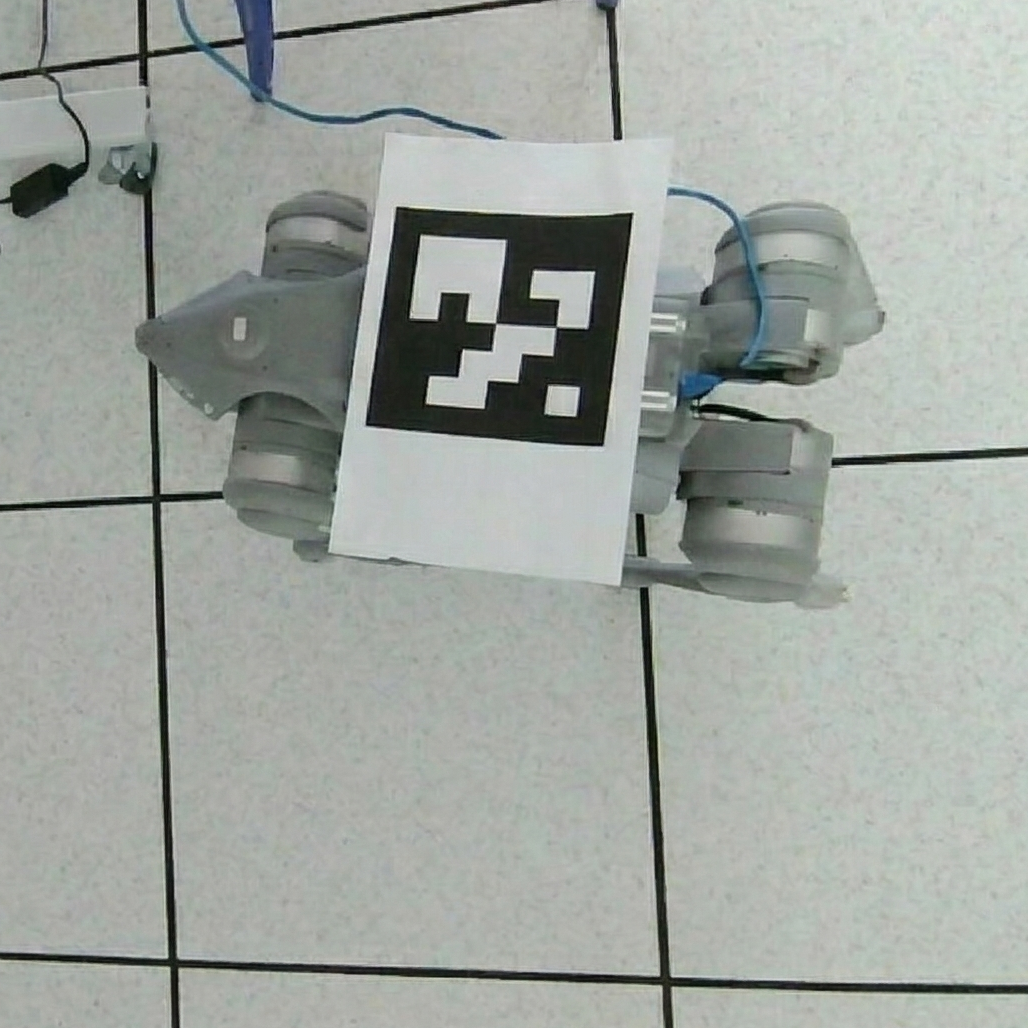
\includegraphics[width=0.62\textwidth]{figures/images/fig_lab_real_fixed_camera.png}
\caption{Montaje experimental de laboratorio utilizado para observar el
movimiento del Go2 real con marcador ArUco, mediante una cámara mantenida en
posición aproximadamente fija.}
\label{fig:method_lab_setup}
\end{figure}

\subsubsection{Comparación entre movimiento esperado, comando y respuesta del robot}

El contraste principal de esta etapa se planteó entre el movimiento objetivo,
el comando efectivamente transmitido y las señales internas publicadas por el
cuadrúpedo. En otras palabras, la comparación no se formuló como una estimación
absoluta de pose respecto del mundo, sino como una verificación de si la
dinámica solicitada por el simulador marino se reflejaba de manera coherente en
la respuesta medida por la propia plataforma. La corrida real versionada permite
seguir esta cadena casi completa: la señal de depuración describe el movimiento esperado,
el tópico de peticiones API deja ver el comando
Euler realmente enviado, y el estado deportivo, el estado de bajo nivel y la odometría
\texttt{utlidar} aportan distintas lecturas del estado del robot
(Tabla~\ref{tab:ros_interfaces_lab}).

Metodológicamente, esta decisión tiene dos ventajas. En primer lugar, permite
comparar directamente la señal propuesta con una señal efectivamente disponible
en el robot real, sin depender de un sistema externo de ground truth. En
segundo lugar, separa el problema en dos niveles: fidelidad del camino de
comando, por un lado, y fidelidad de la respuesta física del cuerpo, por otro.
Así, el laboratorio pasa a funcionar como una validación de correspondencia
entre entrada, actuación y respuesta, más que como una réplica exacta del
esquema de evaluación usado en Gazebo.

En términos operativos, la comparación se apoyó en señales con frecuencias muy
distintas. La depuración del simulador marino se publica a baja frecuencia
como señal de referencia, mientras que la API y el estado del robot quedan
muestreados a frecuencias mucho mayores. Por eso el análisis posterior se
realizó alineando temporalmente señales mediante vecino más cercano o
interpolación, según el caso. En la metodología alcanza con dejar claro que el
objetivo fue contrastar el movimiento propuesto con el camino real de comando y
con la respuesta interna del robot, usando esa relación como primer puente entre
la plataforma sintética de simulación y su comportamiento en entorno real.

\figureplaceholder
  {fig:method_lab_comparison}
  {Gráfico pendiente de comparación entre la señal esperada (depuración del simulador marino),
  el comando Euler enviado por la API Sport Mode y el estado real medido por
  estado deportivo u odometría \texttt{utlidar} (Tabla~\ref{tab:ros_interfaces_lab}). La figura debería
  mostrar series temporales alineadas para ilustrar el criterio de contraste
  entre objetivo, actuación y respuesta.}
  {Esquema de la comparación realizada en laboratorio entre la señal objetivo
  del movimiento, el comando transmitido y la respuesta medida por el
  cuadrúpedo.}



\section{Experimentación y resultados}

Una vez definido el pipeline y explicitados los criterios metodológicos, la
evidencia se presenta como una progresión desde el caso más controlado hasta el
contraste físico. Primero se analizan las corridas de simulación, donde la
referencia reconstruida permite medir el desempeño del estimador con mayor
aislamiento. Luego se presenta el laboratorio, donde el foco deja de estar en
el error frente a ground truth y pasa a la correspondencia entre movimiento
esperado, comando enviado y respuesta del robot.

\subsection{Experimentos en simulación}

Las pruebas en simulación constituyen el núcleo cuantitativo más sólido del
trabajo, porque permiten contrastar la pose estimada visualmente con la pose de
referencia obtenida a partir del simulador. La campaña final se organizó como
una progresión deliberada: primero, un baseline con \texttt{fixed\_camera} para
instalar el caso más limpio del framework; después, tres repeticiones
comparables con \texttt{sjtu\_drone} para estudiar el mismo movimiento bajo una
geometría de observación más exigente. Todas las corridas se registraron en
rosbags de aproximadamente un minuto y se reevaluaron \textit{offline} con el
mismo pipeline.

\subsubsection{Diseño experimental y corridas seleccionadas}

\todo[inline]{Trabajo futuro: incorporar una corrida adicional (p.\,ej.\ R4) con patrón \texttt{irregular} o repetir el escenario \texttt{sinusoidal} con mayor intensidad de movimiento, para aislar el efecto del régimen dinámico sobre el error de detección del marcador.}

Con el fin de aislar el efecto de la fuente de imagen, todas las corridas de
esta subsección comparten la misma consigna de movimiento marino en modo
\texttt{sinusoidal} y los mismos parámetros de referencia ya presentados en la
metodología (Tabla~\ref{tab:method_marine_params}). Sobre esa base fija se
construyó la campaña \texttt{report\_v2}: un baseline con cámara fija y tres
repeticiones comparables del escenario con dron. Esta estructura no se eligió
sólo para acumular más bags, sino para separar con claridad dos preguntas.
Primero, qué tan bien sigue el pipeline visual el movimiento del marcador cuando
el sensor permanece fijo. Segundo, cuánto se degrada esa estimación cuando la
observación pasa a depender también de la pose de un vehículo aéreo.

\begin{table}[H]
\centering
\caption{Corridas seleccionadas para estructurar el capítulo experimental en
simulación. La campaña final instala un baseline con cámara fija y luego
profundiza el escenario con dron mediante tres repeticiones comparables.}
\label{tab:sim_selected_runs}
\begin{adjustbox}{max width=\textwidth}
\begin{tabular}{p{0.14\textwidth}p{0.18\textwidth}p{0.12\textwidth}p{0.17\textwidth}p{0.29\textwidth}}
\toprule
Corrida & Fuente de imagen & Duración & Movimiento & Propósito en el relato experimental \\
\midrule
Baseline fijo & \texttt{fixed\_camera} & 57,5 s & Configuración sinusoidal de referencia & Instalar el caso metodológicamente más limpio y fijar una referencia visual del pipeline. \\
R1 & \texttt{sjtu\_drone} & 57,7 s & Configuración sinusoidal de referencia & Primera repetición comparable del escenario fuerte, con alta disponibilidad de muestras. \\
R2 & \texttt{sjtu\_drone} & 57,4 s & Configuración sinusoidal de referencia & Corrida principal del dron; se usa para las series temporales y los histogramas detallados. \\
R3 & \texttt{sjtu\_drone} & 57,7 s & Configuración sinusoidal de referencia & Tercera repetición comparable del dron; se usa para discutir variabilidad entre ejecuciones equivalentes. \\
\bottomrule
\end{tabular}
\end{adjustbox}
\end{table}

En términos concretos, el baseline y las tres repeticiones del dron corresponden
a los registros listados en la Tabla~\ref{tab:appendix_rosbags} (campaña
\texttt{report\_v2}, abril de 2026). Las cuatro bolsas
se reevaluaron con el mismo pipeline \textit{offline} y con el mismo offset de
spawn del Go2 \((world\_init\_x = 0{,}40)\), de modo que las diferencias
reportadas más adelante no provienen de cambios en el postproceso ni de una
mezcla de implementaciones distintas del escenario.

\subsubsection{Métricas y criterio de lectura}

La evaluación se apoya en un conjunto acotado de métricas que dialogan de forma
directa con el movimiento marino que se quiso sintetizar. En esta campaña se
privilegian tres variables: el error angular en \texttt{roll}, el error angular
en \texttt{pitch} y el error en \texttt{heave}, medido como \(\Delta Z\) en el
frame de la cámara. Estas magnitudes son las que mejor capturan la parte del
problema vinculada con el balanceo, el cabeceo y la variación vertical de la
plataforma. Como descriptores complementarios se conservan la cantidad de
muestras útiles, la tasa de detección y, de forma secundaria, el error
euclidiano de posición \(\|\Delta pos\|\) y la lectura por ejes \(X/Y/Z\).

\begin{table}[H]
\centering
\caption{Resumen cuantitativo de las tres corridas del escenario
\texttt{sjtu\_drone}, calculado a partir de la evaluación \textit{offline}
contra ground truth reconstruido en frame cámara. La tabla prioriza el error
absoluto medio en \texttt{roll}, \texttt{pitch} y \texttt{heave}.}
\label{tab:sim_drone_quant_structure}
\begin{adjustbox}{max width=\textwidth}
\begin{tabular}{p{0.10\textwidth}p{0.12\textwidth}p{0.12\textwidth}p{0.15\textwidth}p{0.15\textwidth}p{0.14\textwidth}p{0.22\textwidth}}
\toprule
Corrida & Muestras & Detección & \(\overline{|\Delta roll|}\) & \(\overline{|\Delta pitch|}\) & \(\overline{|\Delta Z|}\) & Observación sintética \\
\midrule
R1 & 306 & 5,30 Hz & 2,69$^\circ$ & 1,98$^\circ$ & 0,020 m & Mayor disponibilidad de muestras; el error de heave queda levemente más acotado que en las otras repeticiones. \\
R2 & 264 & 4,60 Hz & 3,02$^\circ$ & 2,21$^\circ$ & 0,023 m & Corrida principal; concentra la mayor dispersión angular del grupo y por eso resulta una referencia exigente. \\
R3 & 270 & 4,68 Hz & 2,75$^\circ$ & 2,06$^\circ$ & 0,024 m & Menor error posicional global del grupo, con desempeño angular intermedio y heave comparable a R2. \\
\bottomrule
\end{tabular}
\end{adjustbox}
\end{table}

Conviene leer estas métricas en dos niveles. Primero, como una descripción
local de cada corrida: cuántas detecciones útiles hubo y qué orden de magnitud
alcanzan \texttt{roll}, \texttt{pitch} y \texttt{heave}. Segundo, como una
comparación entre escenarios: el baseline con cámara fija no compite en peso
con el dron, sino que ofrece una base de lectura sobre la cual interpretar por
qué el escenario con sensor móvil resulta más exigente.

\subsubsection{Caso base: cámara fija}

El caso \texttt{fixed\_camera} funciona como baseline metodológico del
framework. Al mantener el sensor en una posición fija respecto del mundo, la
variación visual proviene esencialmente del movimiento del marcador adherido al
Go2. Esto vuelve más legible la relación entre la consigna sinusoidal del torso
y la pose observada del marcador, por lo que este escenario instala la
referencia más limpia antes de pasar al caso con dron.

\begin{figure}[H]
\centering
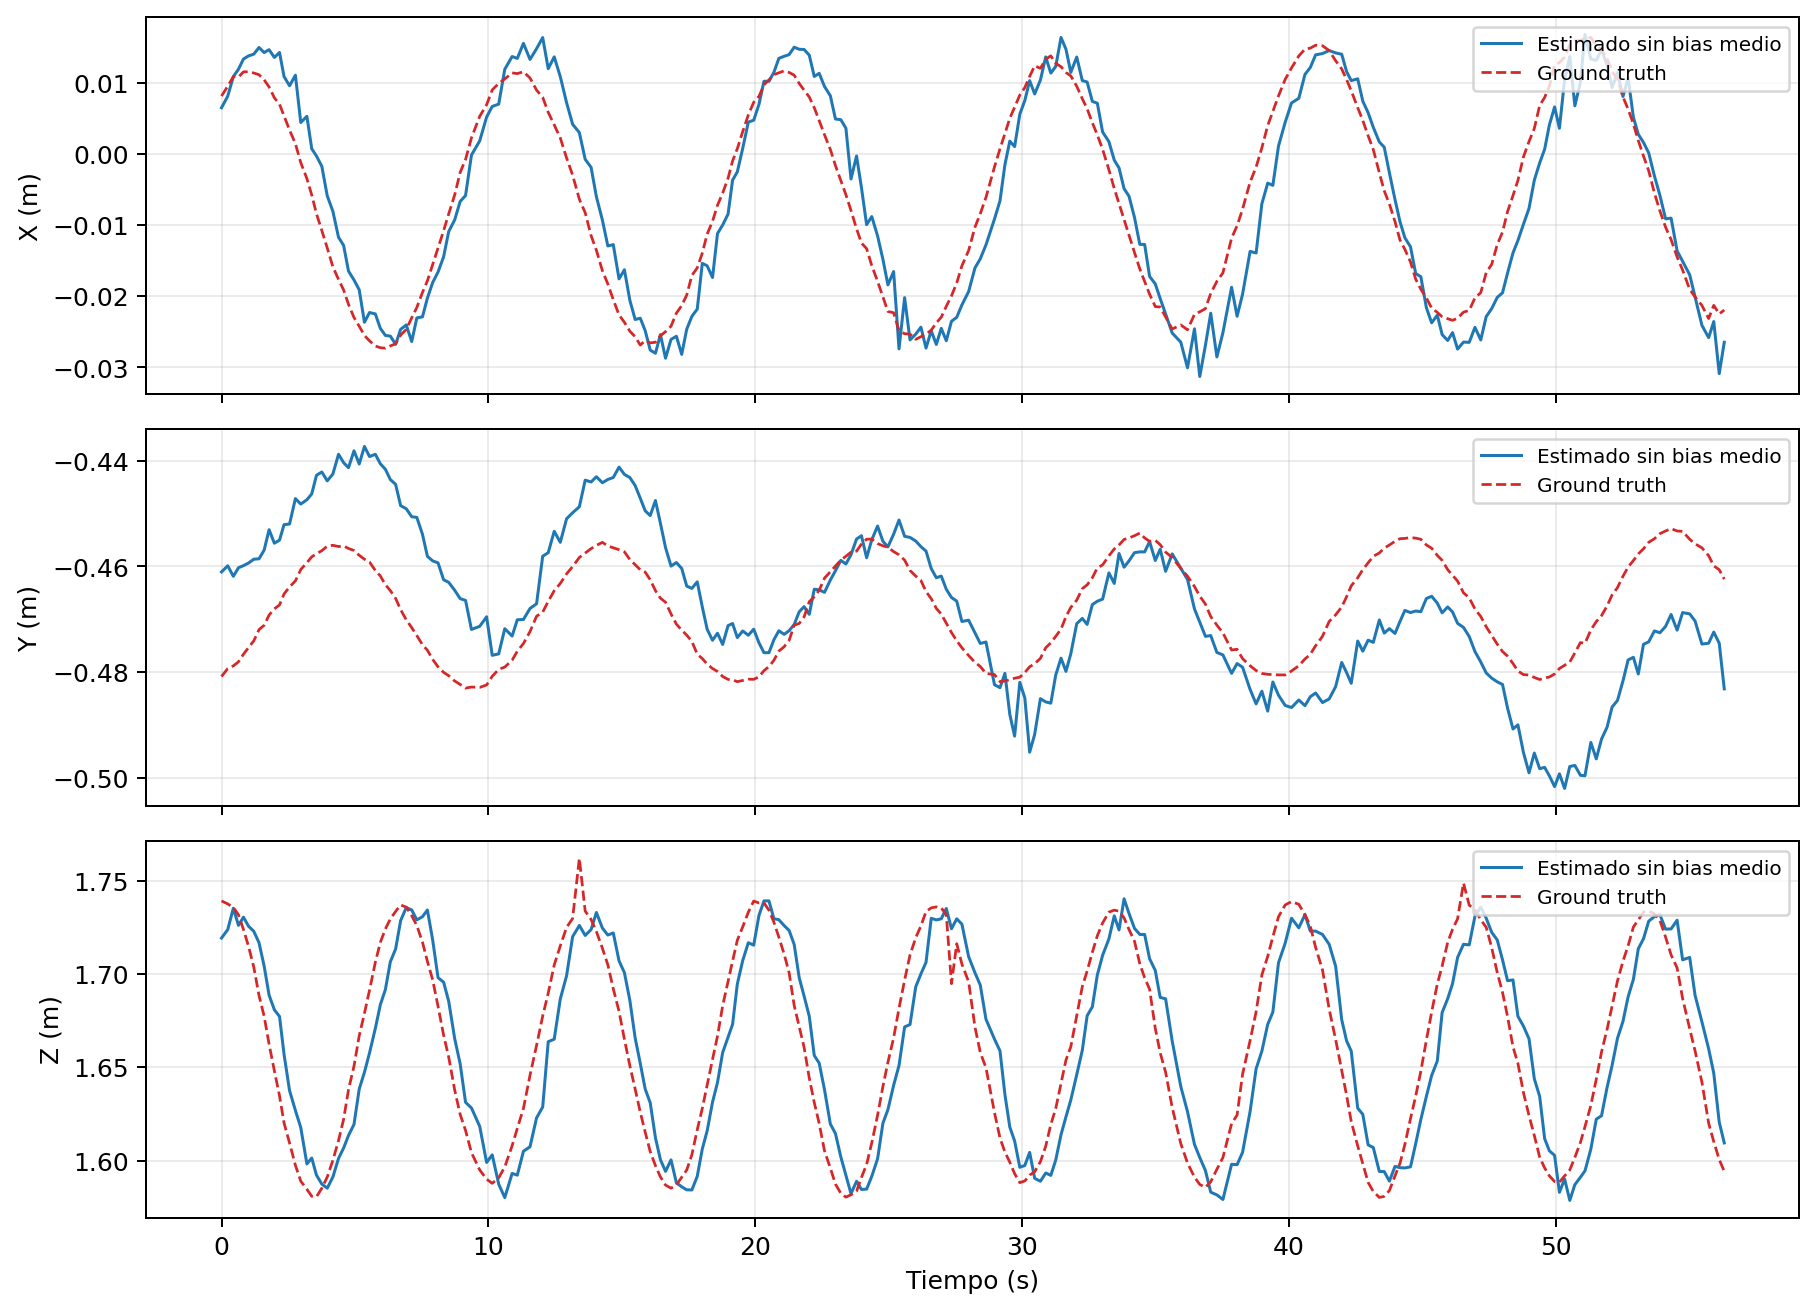
\includegraphics[width=\textwidth]{figures/results/sim_fixed_position_vs_gt.png}
\caption{Comparación temporal entre posición estimada y ground truth en el
escenario base con cámara fija. La señal estimada se muestra sin bias medio por
eje solo para visualización, con el objetivo de facilitar la comparación de
forma y fase entre ambas curvas.}
\label{fig:sim_fixed_position_vs_gt}
\end{figure}

\begin{figure}[H]
\centering
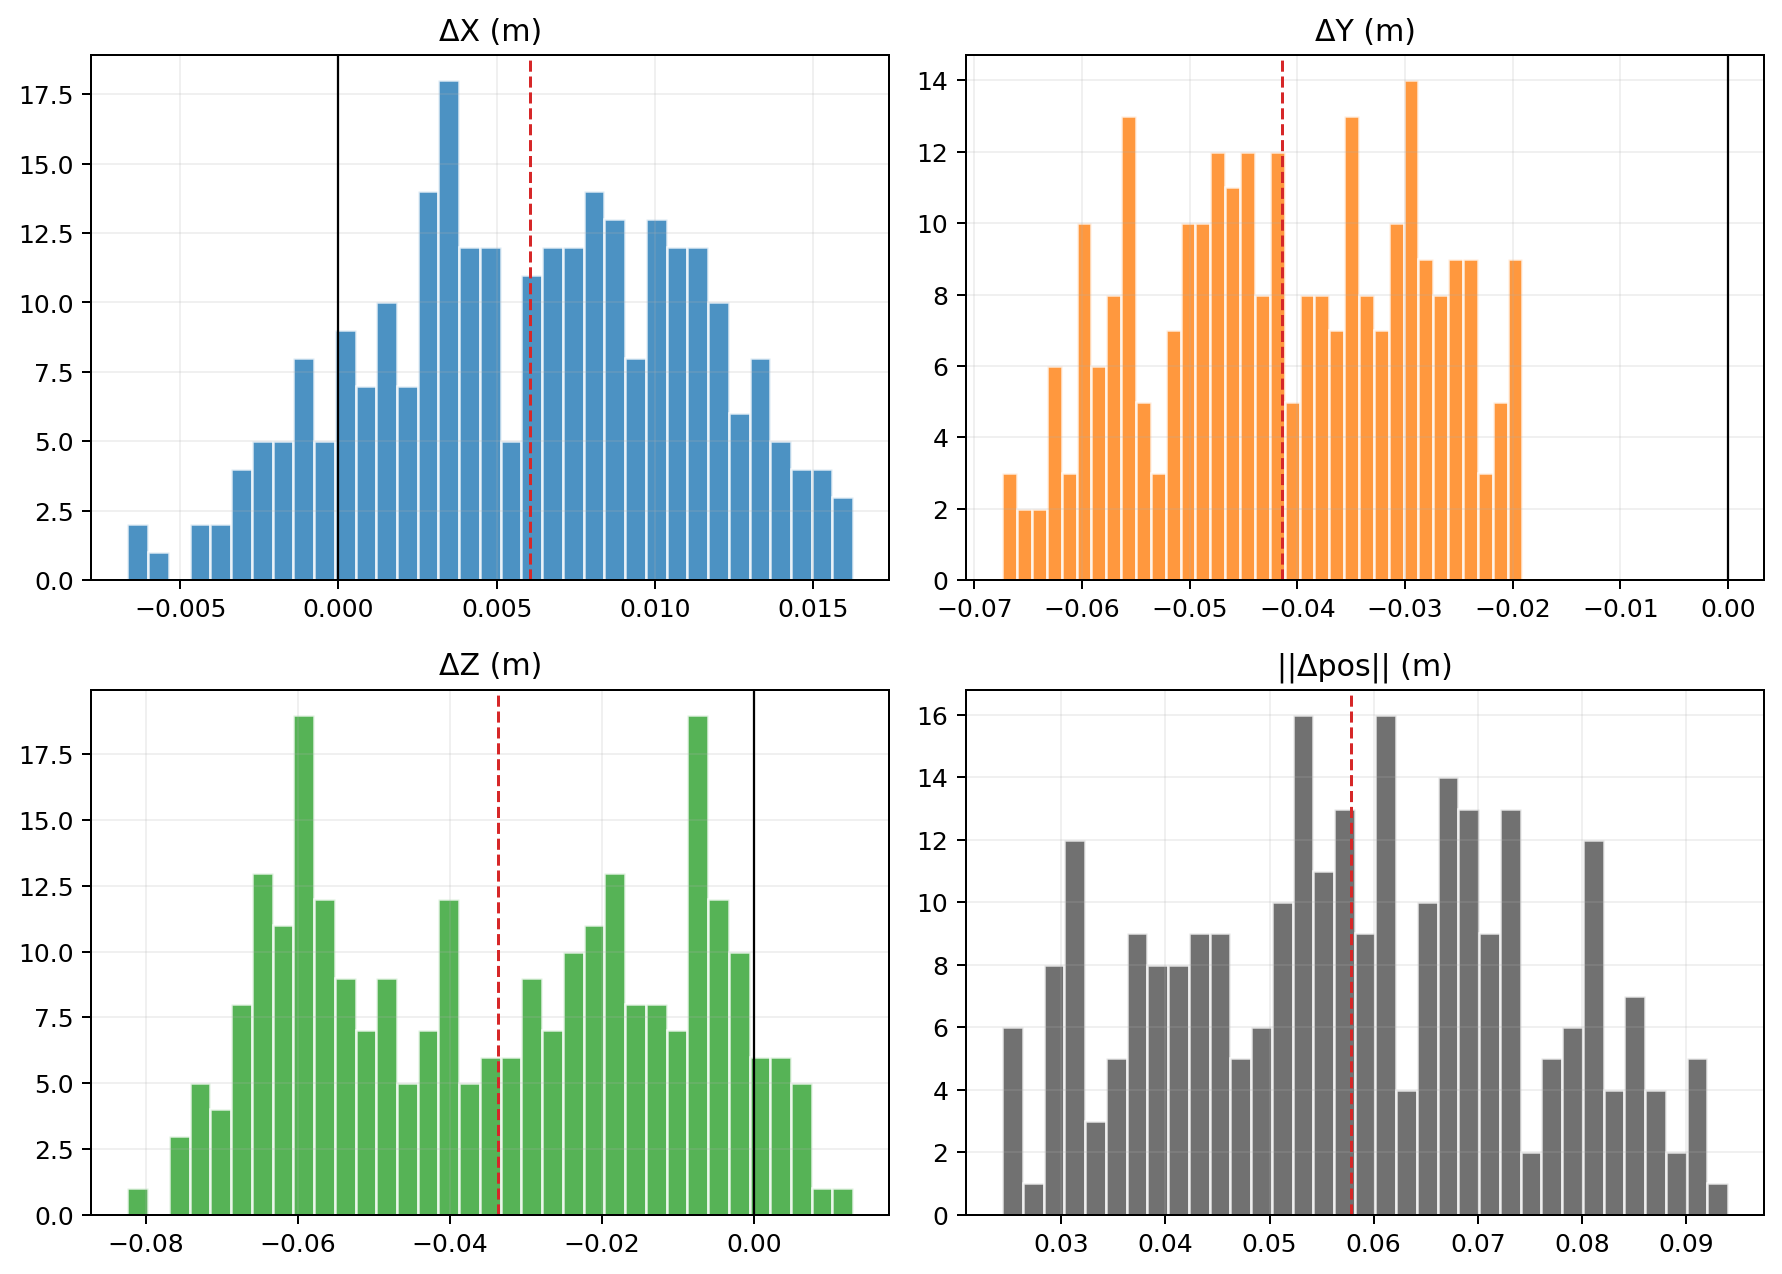
\includegraphics[width=0.92\textwidth]{figures/results/sim_fixed_error_hist.png}
\caption{Distribución de errores de posición en el caso base con cámara fija.
Se muestran \(\Delta X\), \(\Delta Y\), \(\Delta Z\) y el error euclidiano
\(\|\Delta pos\|\), todos calculados sobre la evaluación cruda en frame
cámara.}
\label{fig:sim_fixed_error_hist}
\end{figure}

\begin{figure}[H]
\centering
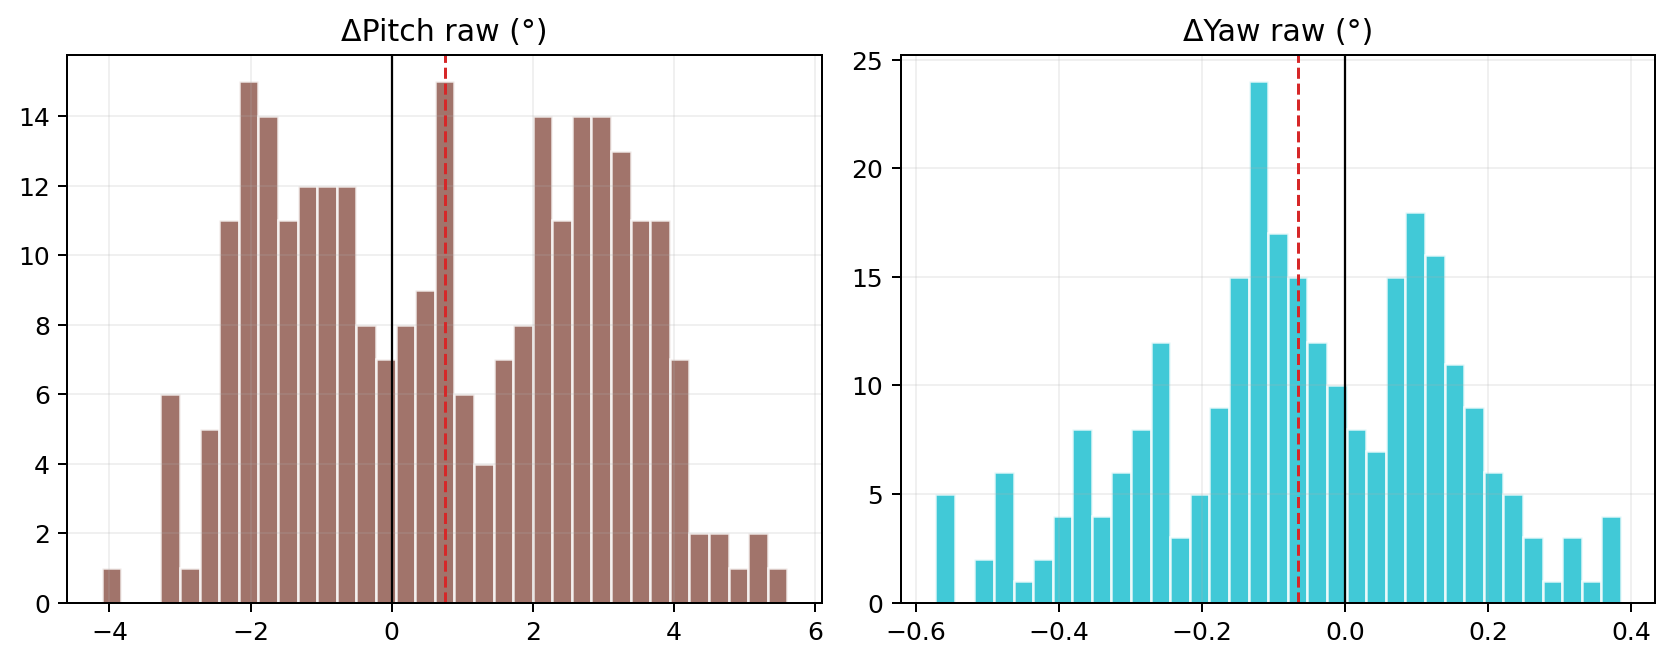
\includegraphics[width=0.82\textwidth]{figures/results/sim_fixed_angle_error_hist_raw.png}
\caption{Distribución raw del error angular en el baseline con cámara fija.
Aquí se muestran \(\Delta pitch\) y \(\Delta yaw\) sin recentrado adicional,
como apoyo para la lectura angular del caso base.}
\label{fig:sim_fixed_angle_error_hist_raw}
\end{figure}

La Figura~\ref{fig:sim_fixed_position_vs_gt} muestra que, en el caso más limpio
del capítulo, la señal estimada reproduce la dinámica global del marcador en
los tres ejes y sigue de forma particularmente clara la componente de heave. El
baseline concentra 275 muestras útiles sobre una corrida de 57,5 s, con una
tasa de detección de 4,78 Hz, de modo que la evidencia visual queda sostenida
por una cantidad de observaciones claramente mayor que en las campañas usadas
en campañas preliminares.

Desde el punto de vista del error, el baseline queda acotado en torno a
\(\mu\|\Delta pos\| = 0{,}0578\) m y \(P95 = 0{,}0853\) m. La componente de
heave concentra la mayor dispersión posicional, con un error absoluto medio de
\(0{,}034\) m, mientras que el error angular se mantiene en torno a
\(2{,}44^\circ\) en \texttt{roll} y \(2{,}00^\circ\) en \texttt{pitch}. El
histograma raw de la Figura~\ref{fig:sim_fixed_angle_error_hist_raw} muestra,
además, que \texttt{yaw} permanece mucho más acotado
\((\overline{|\Delta yaw|} \approx 0{,}17^\circ)\), lo que coincide con la
intuición geométrica de que la rotación planar del marcador es la componente
más estable del problema.

También aparece aquí una limitación que conviene dejar explícita porque luego se
repite en el caso fuerte. En \(Y\), la señal estimada acompaña la fase global
del movimiento, pero el error lateral deriva lentamente a lo largo de la
corrida: su media pasa de aproximadamente \(-0{,}0247\) m en los primeros
10 s a \(-0{,}0571\) m al final, con una pendiente de
\(-0{,}71\) mm/s. Esta caída no refleja un drift equivalente del ground truth,
sino una deriva del error de estimación. Precisamente por eso el baseline
resulta útil: instala una referencia visual limpia y, al mismo tiempo, permite
identificar limitaciones del pipeline antes de agregar la dinámica del dron.

\subsubsection{Caso fuerte: cámara embarcada en el dron}

El escenario con \texttt{sjtu\_drone} concentra el principal interés de la
capítulo, porque introduce una geometría de observación más cercana al problema
que motiva el framework. Aunque en estas corridas el dron no ejecuta todavía un
aterrizaje, su cámara inferior observa una plataforma que oscila y obliga a
analizar la estimación visual en una condición menos ideal que la del caso
fijo. La campaña final se apoyó en tres repeticiones comparables \((R1,\ R2,\
R3)\), de las cuales \(R2\) se adopta como corrida principal porque combina una
cantidad de muestras suficiente con la mayor dispersión angular del grupo, lo
que la vuelve una referencia exigente sin dejar de ser representativa de la
campaña.

\begin{figure}[H]
\centering
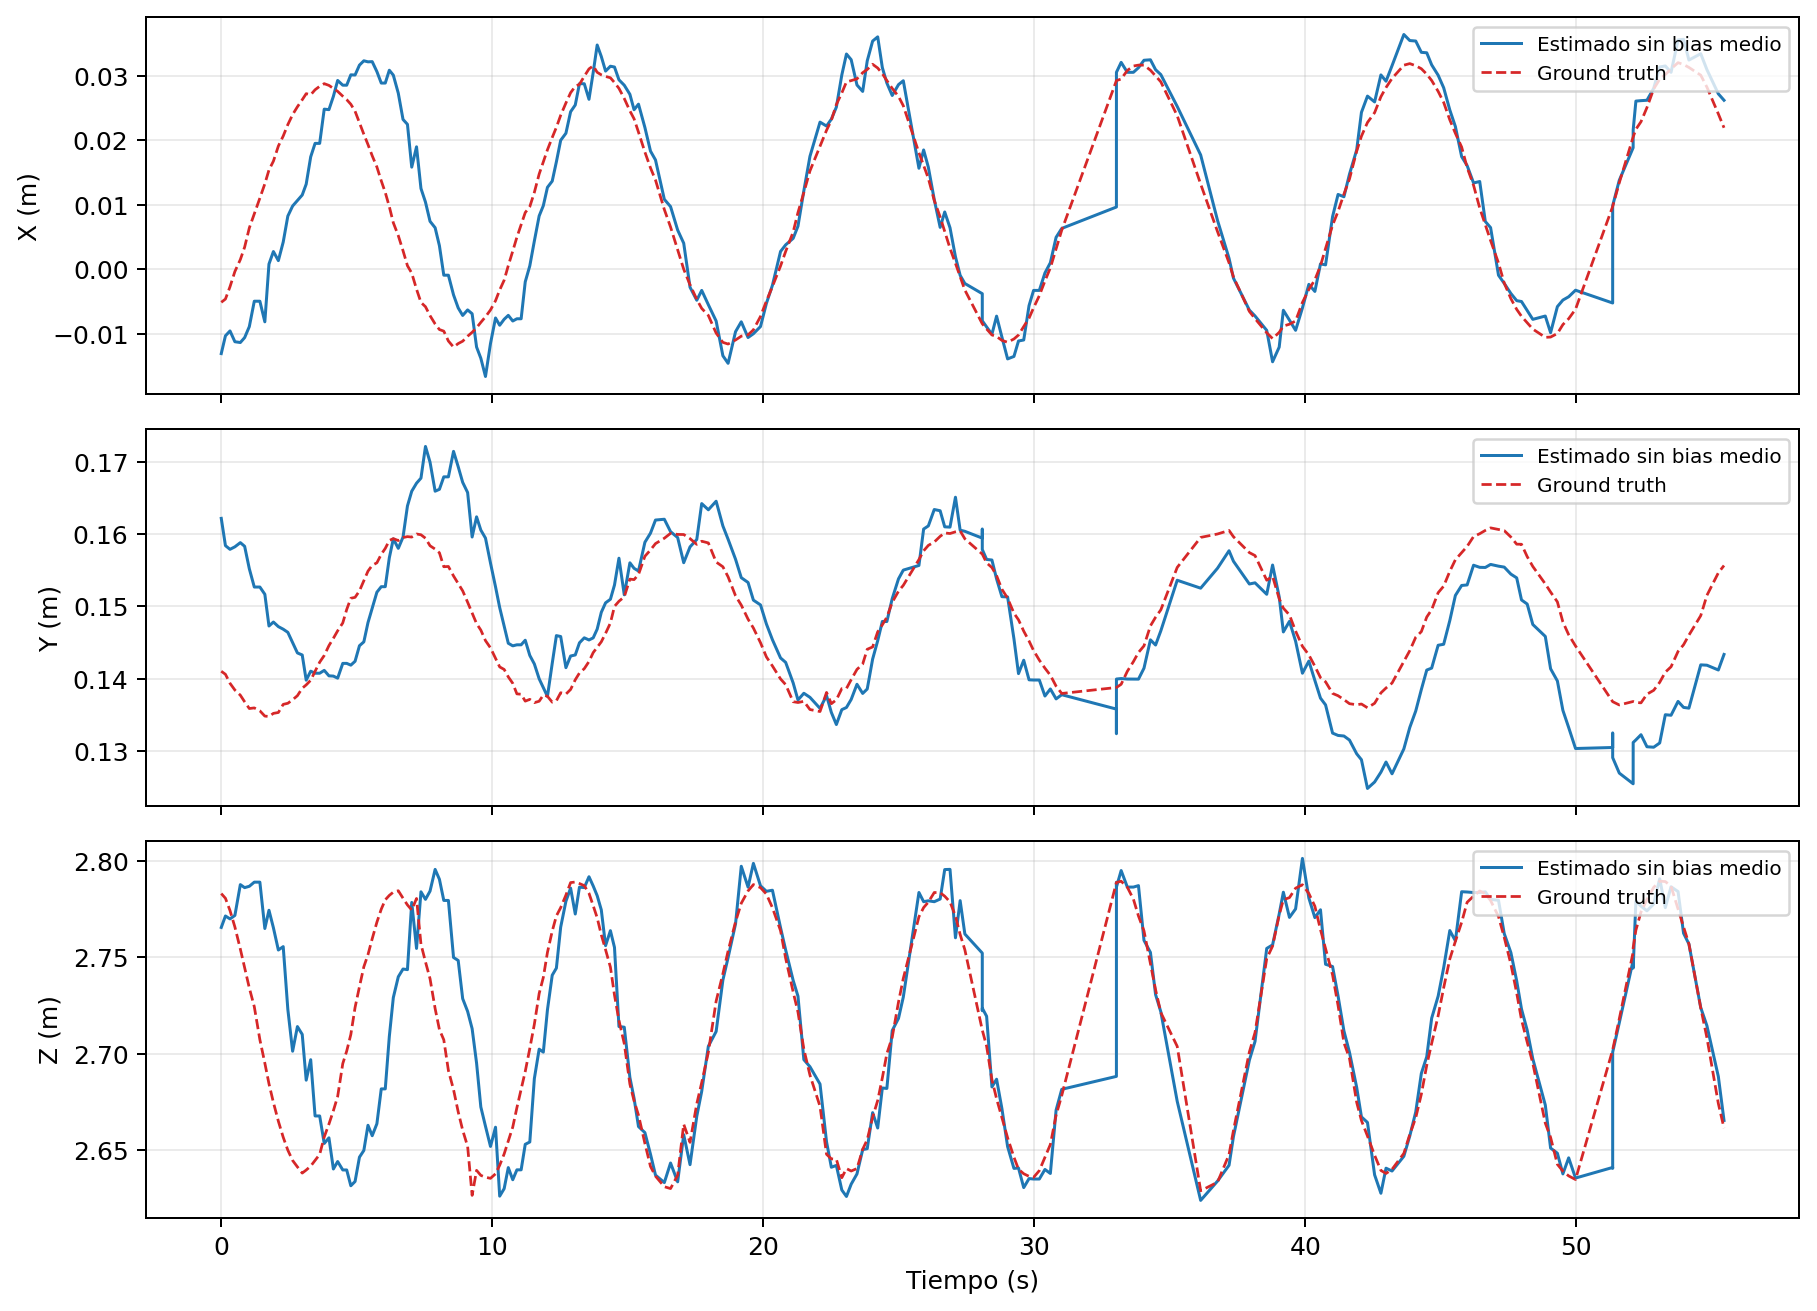
\includegraphics[width=\textwidth]{figures/results/sim_drone_position_vs_gt.png}
\caption{Comparación entre posición estimada y ground truth en la corrida
principal del escenario con dron \((R2)\). La señal estimada se muestra sin
bias medio por eje solo para visualización, de modo de facilitar la lectura de
fase y forma temporal.}
\label{fig:sim_drone_position_vs_gt}
\end{figure}

\begin{figure}[H]
\centering
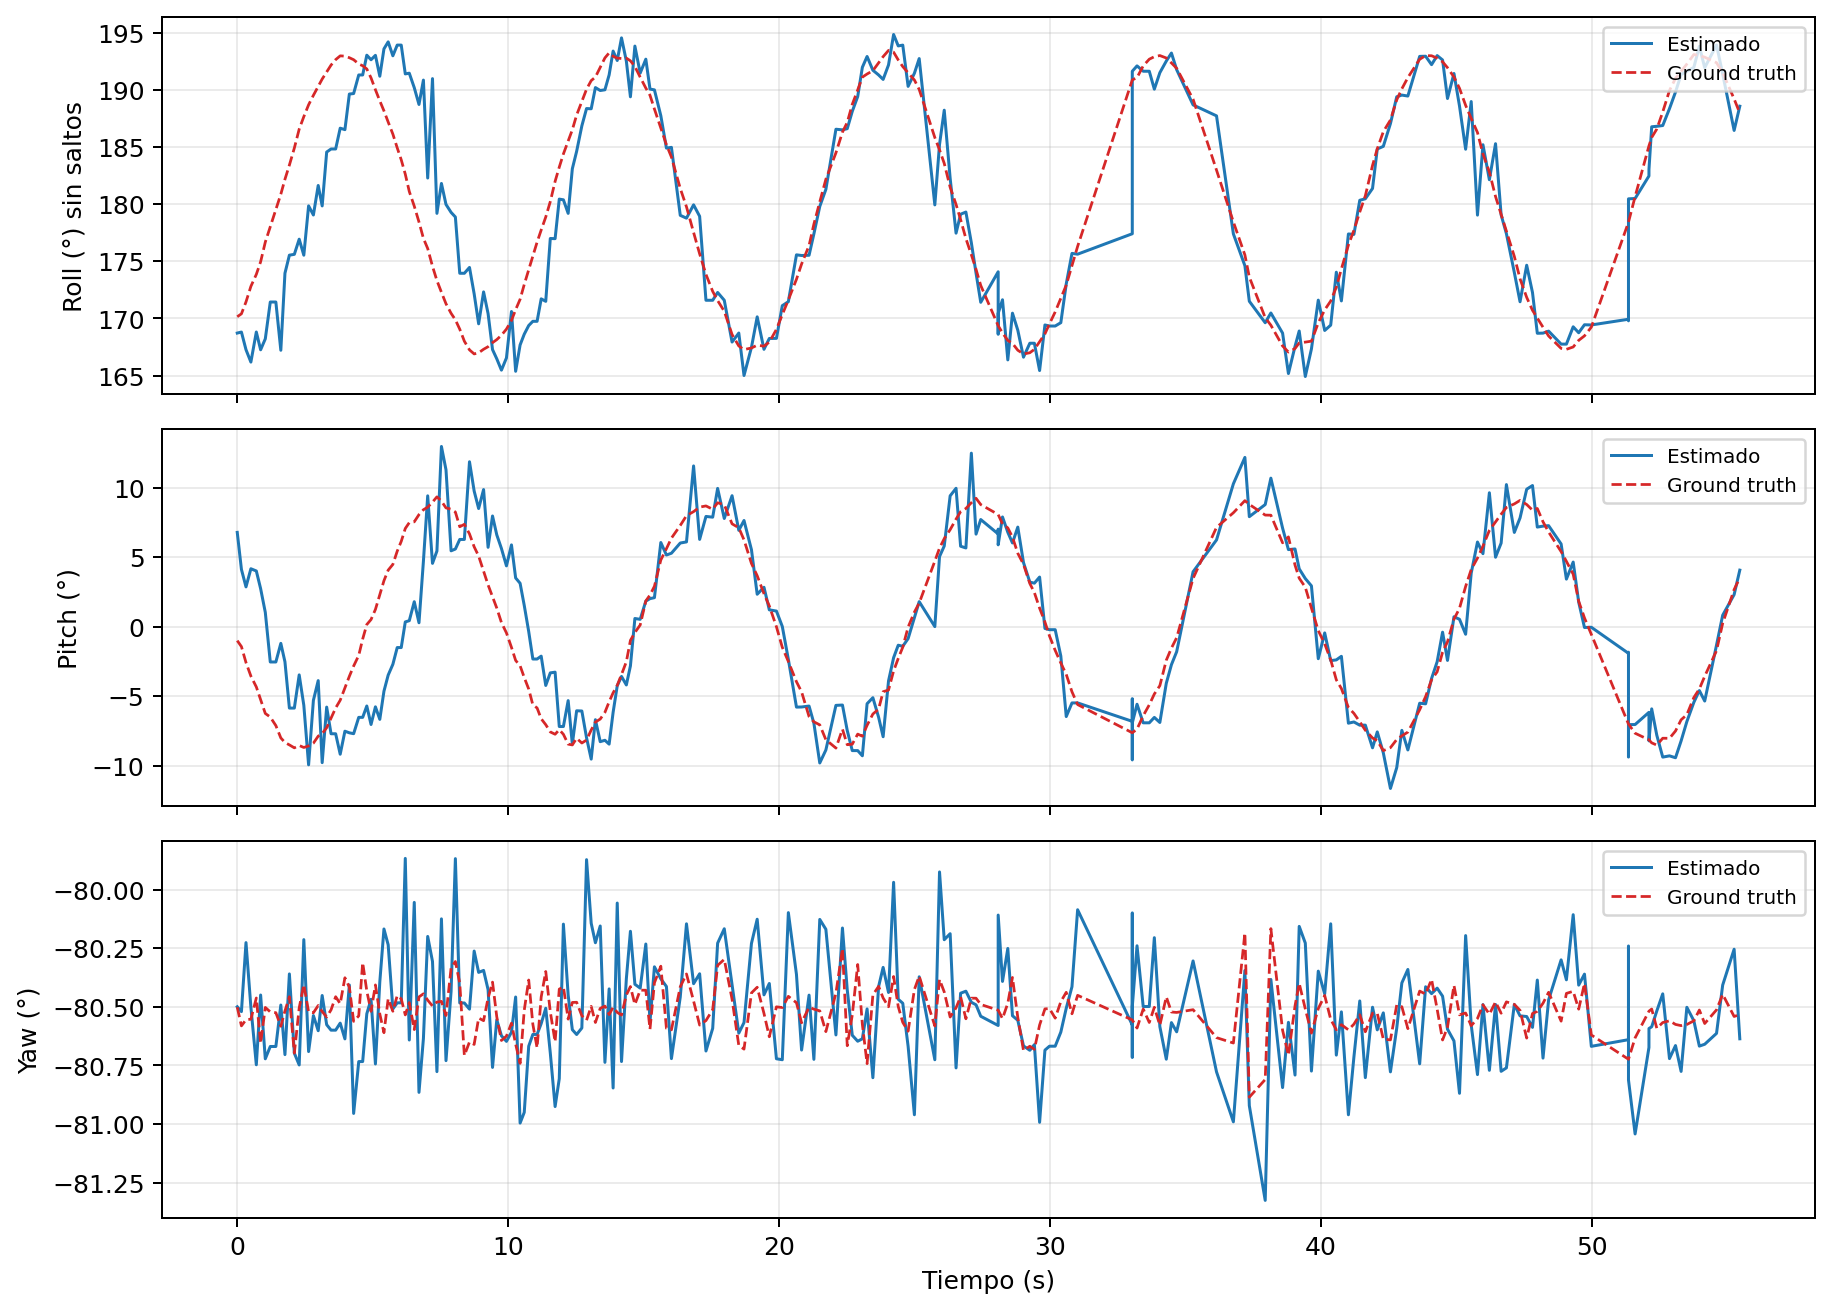
\includegraphics[width=\textwidth]{figures/results/sim_drone_orientation_vs_gt.png}
\caption{Comparación entre orientación estimada y ground truth en la corrida
principal con cámara embarcada en el dron. En \texttt{roll} se aplica
\textit{unwrap} angular solo para visualización, con el fin de evitar los
saltos artificiales asociados a la discontinuidad en \(\pm 180^\circ\).}
\label{fig:sim_drone_orientation_vs_gt}
\end{figure}

\begin{figure}[H]
\centering
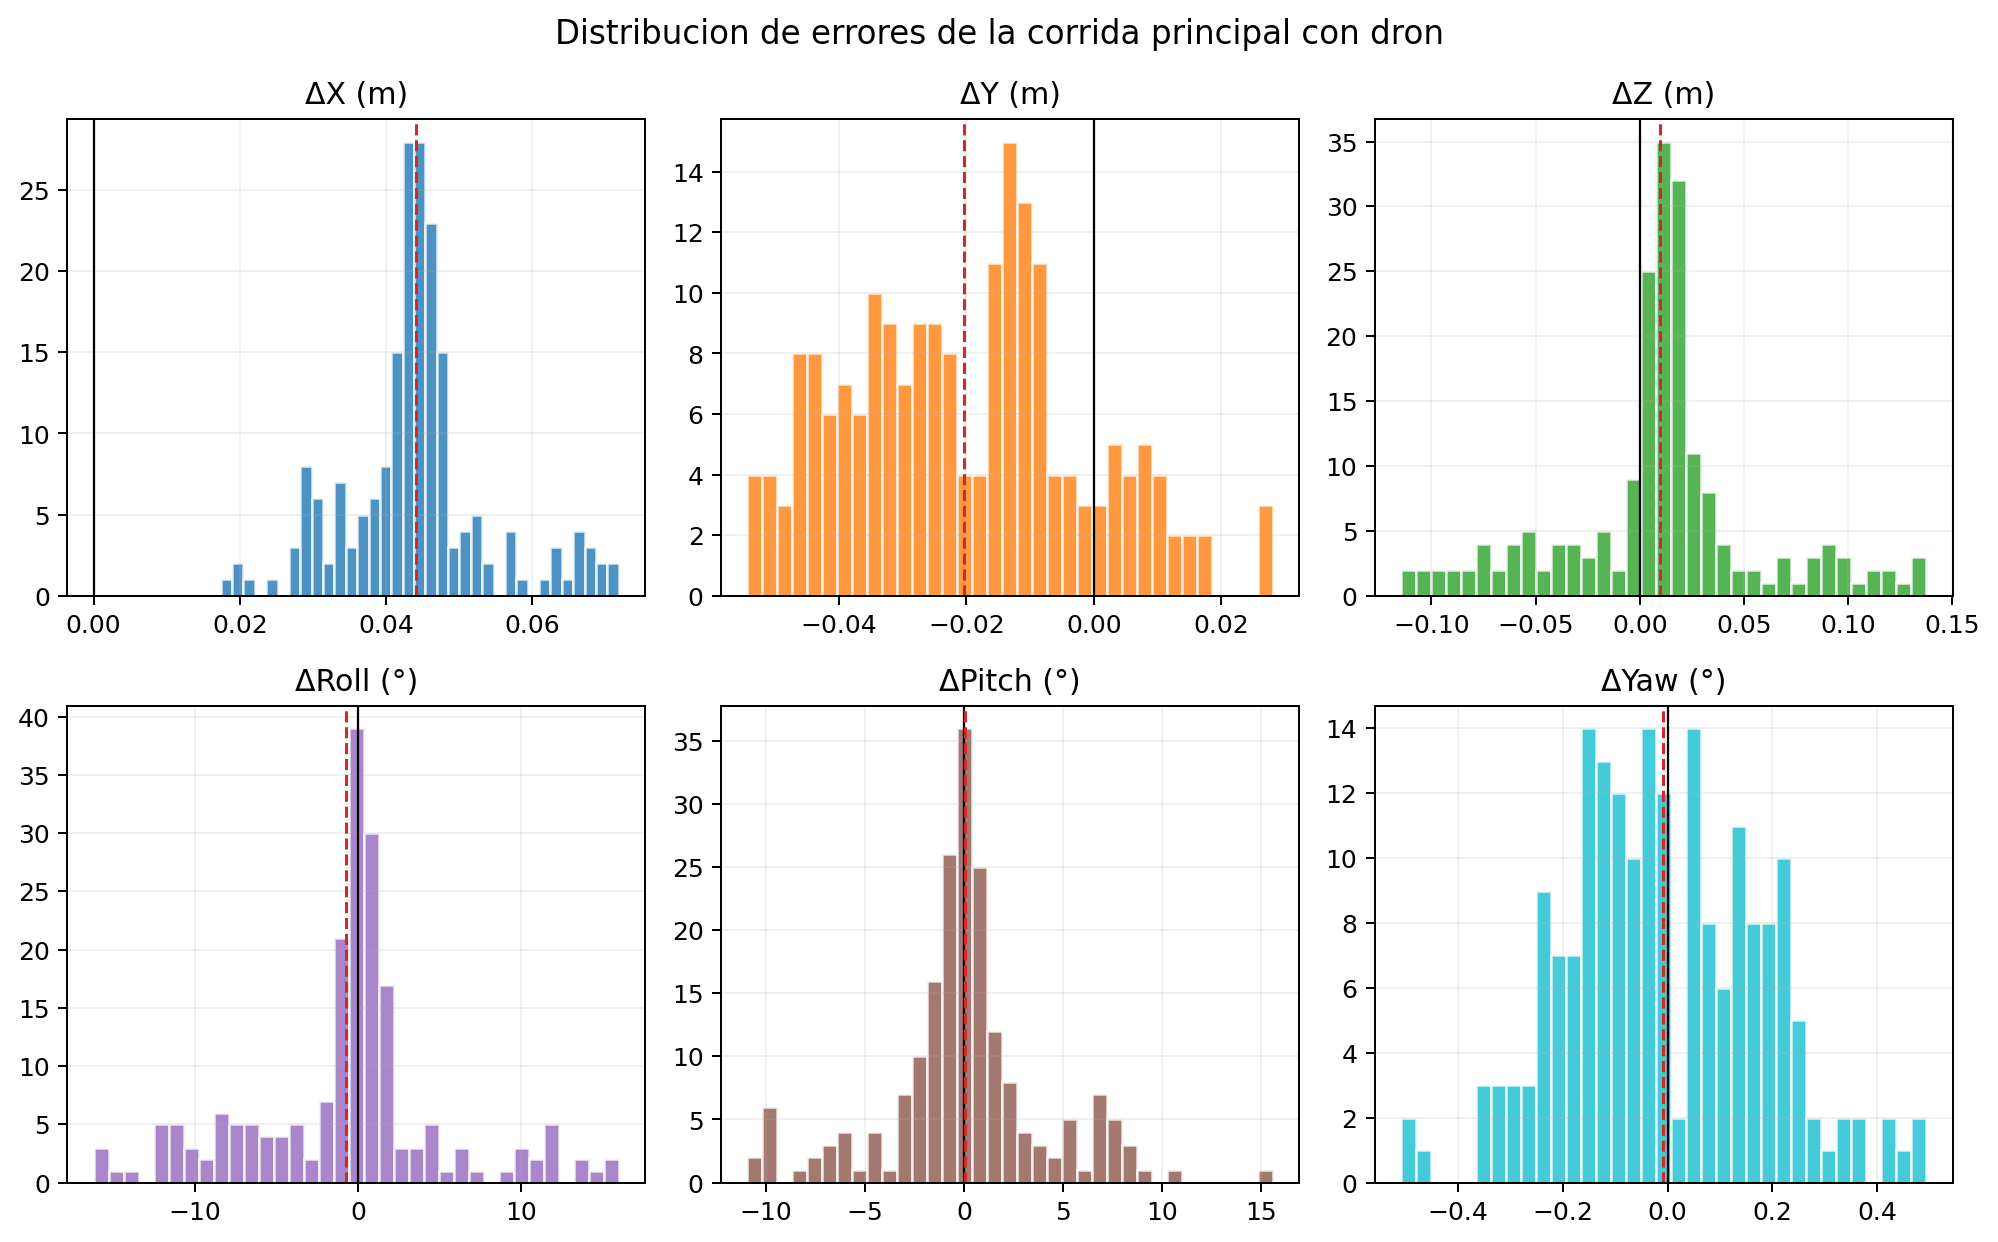
\includegraphics[width=\textwidth]{figures/results/sim_drone_error_hist.png}
\caption{Distribución de errores crudos de la corrida principal del escenario
con dron. La figura resume sesgo y dispersión para las componentes de posición
y orientación estimadas en frame cámara.}
\label{fig:sim_drone_error_hist}
\end{figure}

\begin{figure}[H]
\centering

\includegraphics[width=\textwidth]{figures/results/sim_drone_runs_comparison.png}
\caption{Comparación entre las tres corridas del escenario con dron. Se
muestran boxplots de error absoluto en las variables que más interesan para la
lectura marina del problema: \(|\Delta roll|\), \(|\Delta pitch|\) y
\(|\Delta heave| = |\Delta Z|\).}
\label{fig:sim_drone_runs_comparison}
\end{figure}

La corrida principal del dron, mostrada en las
Figuras~\ref{fig:sim_drone_position_vs_gt} y
\ref{fig:sim_drone_orientation_vs_gt}, conserva la capacidad de seguir la
dinámica global del marcador, pero lo hace bajo una geometría de observación
menos favorable que la del caso fijo. En particular, la figura de posición
permite ver que la señal estimada acompaña la periodicidad dominante en
\texttt{heave} y conserva la estructura temporal en \(X\) y \(Z\), aun cuando
la nube de observaciones aparece más abierta que en el baseline. La figura de
orientación refuerza esa lectura: \texttt{roll} y \texttt{pitch} siguen la
oscilación principal del movimiento, mientras que \texttt{yaw} permanece
acotado y estable, aunque ya no cumple un rol central en la narrativa del
capítulo.

Cuantitativamente, la corrida \(R2\) queda en
\(\overline{|\Delta roll|} = 3{,}02^\circ\),
\(\overline{|\Delta pitch|} = 2{,}21^\circ\) y
\(\overline{|\Delta Z|} = 0{,}023\) m. Estas tres magnitudes son las que mejor
describen cuánto se degrada la observación cuando el sensor pasa de estar fijo
a estar embarcado en un vehículo aéreo. En ese sentido, el escenario con dron
sigue siendo utilizable como banco de pruebas controlado: no pierde la dinámica
global del marcador, pero sí vuelve visibles las componentes más sensibles del
problema visual.

La principal limitación aparece en la posición absoluta y no en la forma
temporal de las oscilaciones. En las tres corridas del dron persiste un sesgo
sistemático en \(Y\), de signo negativo, que alcanza
\(-0{,}322\) m en \(R1\), \(-0{,}297\) m en \(R2\) y \(-0{,}151\) m en \(R3\).
Por eso la lectura principal del capítulo no se apoya en la posición cruda,
sino en la comparación de \texttt{roll}, \texttt{pitch} y \texttt{heave}. Las
figuras de posición, además, se muestran sin bias medio por eje solo para
visualización; los histogramas y tablas conservan siempre los errores crudos.

La comparación entre \(R1\), \(R2\) y \(R3\), resumida en la
Tabla~\ref{tab:sim_drone_quant_structure} y en la
Figura~\ref{fig:sim_drone_runs_comparison}, muestra que el escenario con dron
es comparable entre repeticiones, aunque no idéntico. Las tres corridas se
mantienen en el mismo orden de magnitud, con medianas de
\(|\Delta roll|\) entre \(1{,}63^\circ\) y \(1{,}70^\circ\), medianas de
\(|\Delta pitch|\) entre \(1{,}19^\circ\) y \(1{,}44^\circ\), y medianas de
\(|\Delta Z|\) entre \(0{,}0106\) m y \(0{,}0133\) m. La diferencia principal
aparece en \(R2\), que concentra la mayor dispersión angular del grupo, mientras
que \(R1\) ofrece la mayor tasa de detección y el heave más acotado. \(R3\), en
cambio, mantiene una dispersión angular intermedia y a la vez reduce de forma
marcada el error posicional global, lo que muestra que la repetibilidad del
escenario es razonable pero sensible a la geometría efectiva de cada corrida.

\subsubsection{Síntesis de la evidencia en simulación}

La evidencia de simulación aporta dos conclusiones centrales al argumento
general del trabajo. En primer lugar, la campaña \texttt{report\_v2} confirma
que el pipeline visual sigue la dinámica global de una plataforma oscilante y
que esa capacidad puede medirse con referencia reconstruible. En segundo lugar,
la repetición del escenario con dron muestra que esa lectura no depende de una
única corrida aislada, sino de tres ejecuciones comparables que conservan el
mismo orden de magnitud en \texttt{roll}, \texttt{pitch} y \texttt{heave}.

En conjunto, la evidencia de simulación permite afirmar que el framework sirve
como banco de pruebas controlado para percepción visual sobre plataformas
oscilantes. El baseline fijo instala una referencia limpia, con un error medio
de posición de 5,8 cm y una recuperación clara de la componente de heave;
mientras que el escenario con dron conserva la dinámica global del problema en
una condición más exigente, con errores absolutos medios de alrededor de
\(2^\circ\) a \(3^\circ\) en \texttt{roll}/\texttt{pitch} y de 2 a 2,4 cm en
\texttt{heave}. Esta evidencia alcanza para justificar el valor metodológico de
la simulación como paso previo a la discusión experimental del entorno físico.

Las limitaciones también quedan claras. La componente de heave sigue siendo la
parte posicional más sensible del problema, \texttt{roll} y \texttt{pitch} se
degradan de forma visible cuando la geometría de observación se vuelve menos
favorable, y en el escenario con dron persiste un sesgo sistemático en
\(Y\) que no debe interpretarse como movimiento real de la plataforma, sino
como una limitación actual de la cadena geométrica de estimación y evaluación.
Precisamente por eso la simulación cumple su función metodológica: permite
aislar estas limitaciones con ground truth antes de trasladar la discusión a un
entorno físico.

\subsection{Experimentos en laboratorio}

La validación en laboratorio no replica el mismo esquema de lectura que la
simulación, porque ya no dispone de un ground truth geométrico equivalente. Su
pregunta es otra: hasta qué punto el movimiento propuesto al cuadrúpedo se
refleja en señales observables del sistema. Por eso, en esta etapa el análisis
se apoya en la señal esperada, el comando efectivamente enviado y la respuesta
interna publicada por el robot, además del montaje visual con ArUco y cámara
cuasi fija descripto en la metodología. La implementación real aporta un setup
ROS2 dedicado, un bag versionado y un reporte cuantitativo suficientemente
detallado como para cerrar una primera lectura experimental del caso físico.

\subsubsection{Presentación del material experimental}

El material principal de esta subsección proviene del registro de laboratorio
citado en la Tabla~\ref{tab:appendix_rosbags}, grabado el \mbox{20 de marzo de 2026}.
La corrida dura aproximadamente \(59{,}7\)~s y reúne del orden de \(1{,}59 \times 10^{5}\) mensajes, combinando señal de referencia, comandos enviados a la
API del robot y telemetría de estado. Ese registro alcanza para reconstruir la
cadena completa del experimento: qué movimiento se quería producir, qué comando
se envió efectivamente y cómo respondió el cuerpo del Go2.

\begin{table}[H]
\centering
\caption{Señales principales utilizadas en la corrida real de referencia del
20 de marzo de 2026. Los tópicos completos coinciden con la
Tabla~\ref{tab:ros_interfaces_lab}.}
\label{tab:lab_signals_summary}
\begin{tabular}{p{0.24\textwidth}p{0.16\textwidth}p{0.14\textwidth}p{0.34\textwidth}}
\toprule
Señal (rol) & Mensajes & Tasa aprox. & Rol en el análisis \\
\midrule
Depuración simulador marino & 120 & 2.00 Hz & Movimiento esperado publicado por el simulador marino en modo real \\
Peticiones API (\texttt{api\_id=1007}) & 2968 & 49.70 Hz & Comando Euler efectivamente enviado al robot \\
Estado deportivo & 29671 & 498.02 Hz & Estado principal del robot: actitud, altura del tronco y gait \\
Estado bajo nivel & 29788 & 499.77 Hz & Señal alternativa de estado e IMU interna \\
Odometría \texttt{utlidar} & 14461 & 242.73 Hz & Odometría externa al pipeline de Sport Mode, usada como contraste adicional \\
\bottomrule
\end{tabular}
\end{table}

El montaje físico de esa corrida conserva la lógica general descripta en la
metodología: marcador ArUco adherido al lomo del Go2, cámara estéreo utilizada
en modo monocular, calibración previa del sensor y posición aproximadamente fija
por encima del robot. En paralelo, el sistema visual quedó preparado para
grabar imagen y calibración del estéreo, además de las salidas del detector ArUco
(Tablas~\ref{tab:ros_interfaces_sim} y \ref{tab:ros_interfaces_lab}). Sin embargo, la evidencia cuantitativa
versionada disponible se concentra en la reproducción del movimiento y en la
respuesta del robot, no todavía en un cierre estadístico completo de la
pose visual real. El montaje puede verse en la Figura~\ref{fig:method_lab_setup}.

\subsubsection{Fidelidad del camino de comando}

Antes de discutir la respuesta física del robot, verificamos si la
consigna generada por el simulador marino llega al Go2 sin degradarse. Para eso
se comparó la señal de depuración del simulador marino con los mensajes de
peticiones API correspondientes al comando Euler
(\texttt{api\_id=1007}; Tabla~\ref{tab:ros_interfaces_lab}). La alineación temporal se hizo por vecino más cercano,
porque ambas señales representan el mismo comando en frecuencias distintas.

\begin{table}[H]
\centering
\caption{Resultados principales de la comparación entre la señal esperada y el
comando API efectivamente enviado al robot en la corrida real de referencia.}
\label{tab:lab_command_fidelity}
\begin{tabular}{p{0.42\textwidth}p{0.24\textwidth}p{0.20\textwidth}}
\toprule
Métrica & Roll / eje \(x\) & Pitch / eje \(y\) \\
\midrule
Correlación señal esperada vs API & 0.999887 & 0.999909 \\
RMSE entre señal esperada y API & 0.00261 rad & 0.00188 rad \\
\bottomrule
\end{tabular}
\end{table}

Además de esas correlaciones casi unitarias, el desfase temporal medio entre la
señal esperada y el comando API fue de \texttt{4.98 ms}, con un máximo de
\texttt{10.18 ms}. Esta verificación es metodológicamente importante porque
muestra que el primer eslabón del pipeline real ---la generación y envío del
comando--- no es el principal cuello de botella del experimento. La diferencia
entre objetivo y respuesta debe buscarse, entonces, en la dinámica física del
robot y no en una mala transferencia de la consigna.

\begin{figure}[H]
\centering
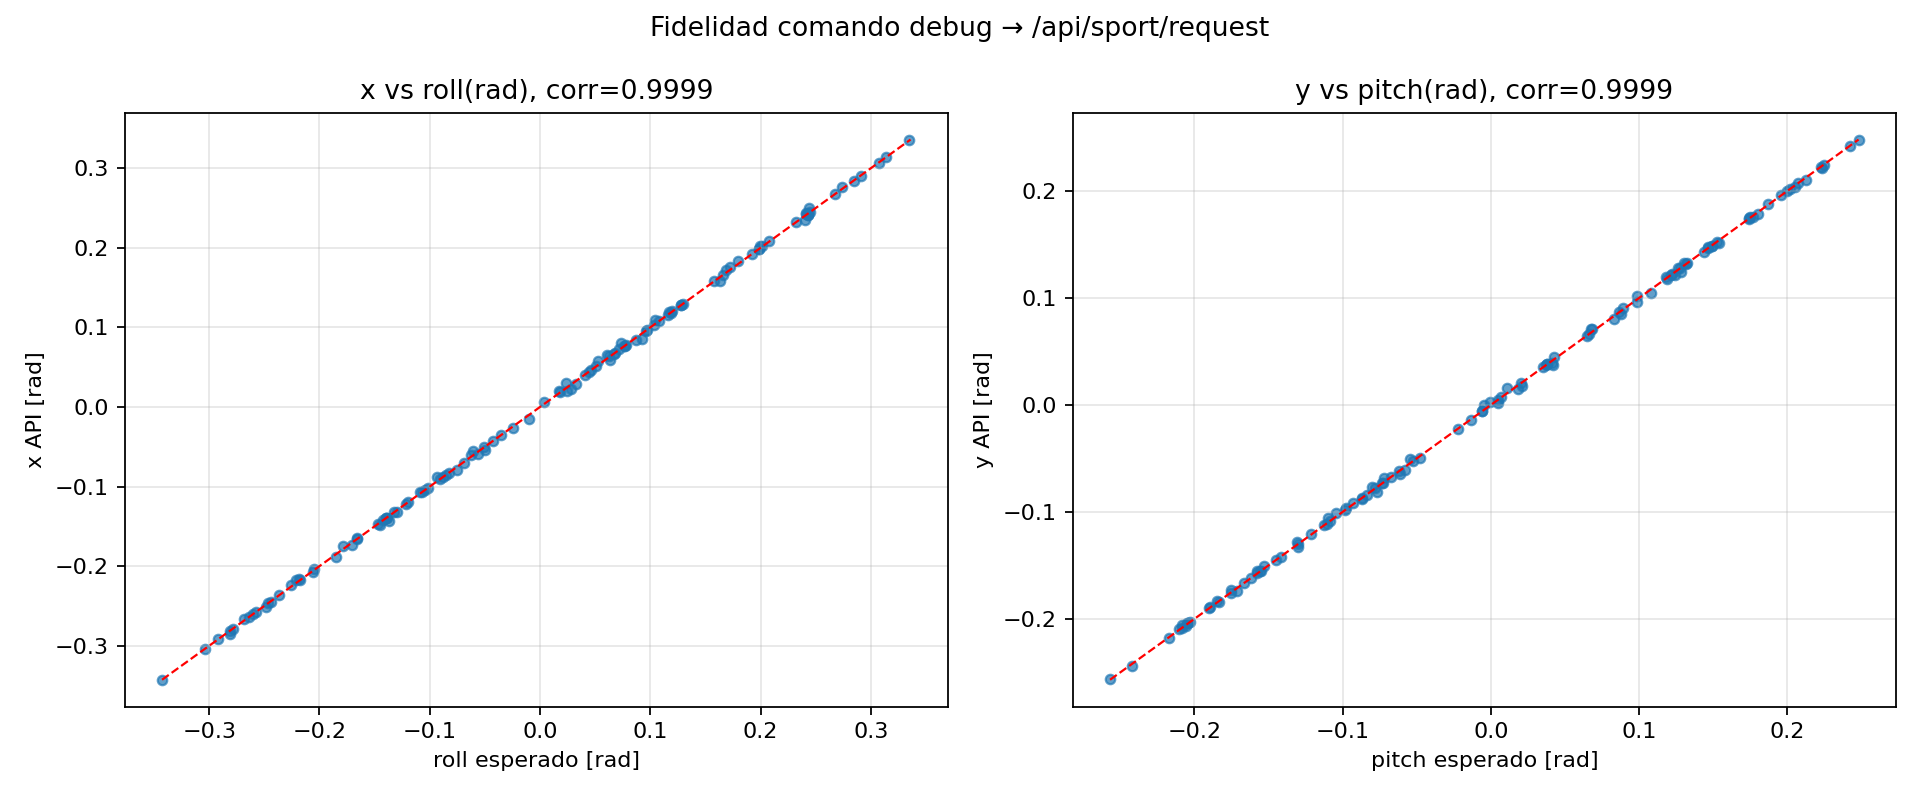
\includegraphics[width=\textwidth]{figures/images/lab_plot_02_api_fidelity.png}
\caption{Fidelidad del camino de comando entre la señal esperada del simulador
marino y el comando Euler enviado al Go2 real. Cada panel compara la consigna
angular con el valor transmitido por la API Sport Mode para el eje
correspondiente, lo que permite visualizar la cercanía a la diagonal identidad.}
\label{fig:lab_api_fidelity}
\end{figure}

\subsubsection{Comparación entre movimiento objetivo y respuesta del robot}

Una vez validado el camino de comando, el segundo bloque se concentra en la
respuesta real del robot. La señal esperada, tomada del tópico de depuración del simulador marino, muestra en esta corrida un movimiento
dominante de \(0{,}15\)~Hz, con rangos de \(-19.637^\circ\) a
\(19.173^\circ\) en roll y de \(-14.719^\circ\) a \(14.212^\circ\) en pitch.
En cambio, la componente vertical de esa señal permaneció en cero durante toda
la secuencia, de modo que el ensayo versionado quedó principalmente orientado a
evaluar la reproducción de roll y pitch.

La respuesta interna del robot se leyó desde tres fuentes complementarias
(estado deportivo, estado de bajo nivel y odometría \texttt{utlidar};
Tabla~\ref{tab:ros_interfaces_lab}). Para poder compararlas con la señal de referencia
se interpoló el estado real al tiempo de muestreo de la depuración del simulador
y luego se calcularon correlaciones tanto a retardo cero como con búsqueda de
lag en una ventana de \(\pm 3\) segundos. Esa estrategia permite distinguir dos
efectos distintos: por un lado, cuánto se parece la forma general del
movimiento; por otro, cuánto retardo dinámico introduce el sistema físico.

\begin{figure}[H]
\centering
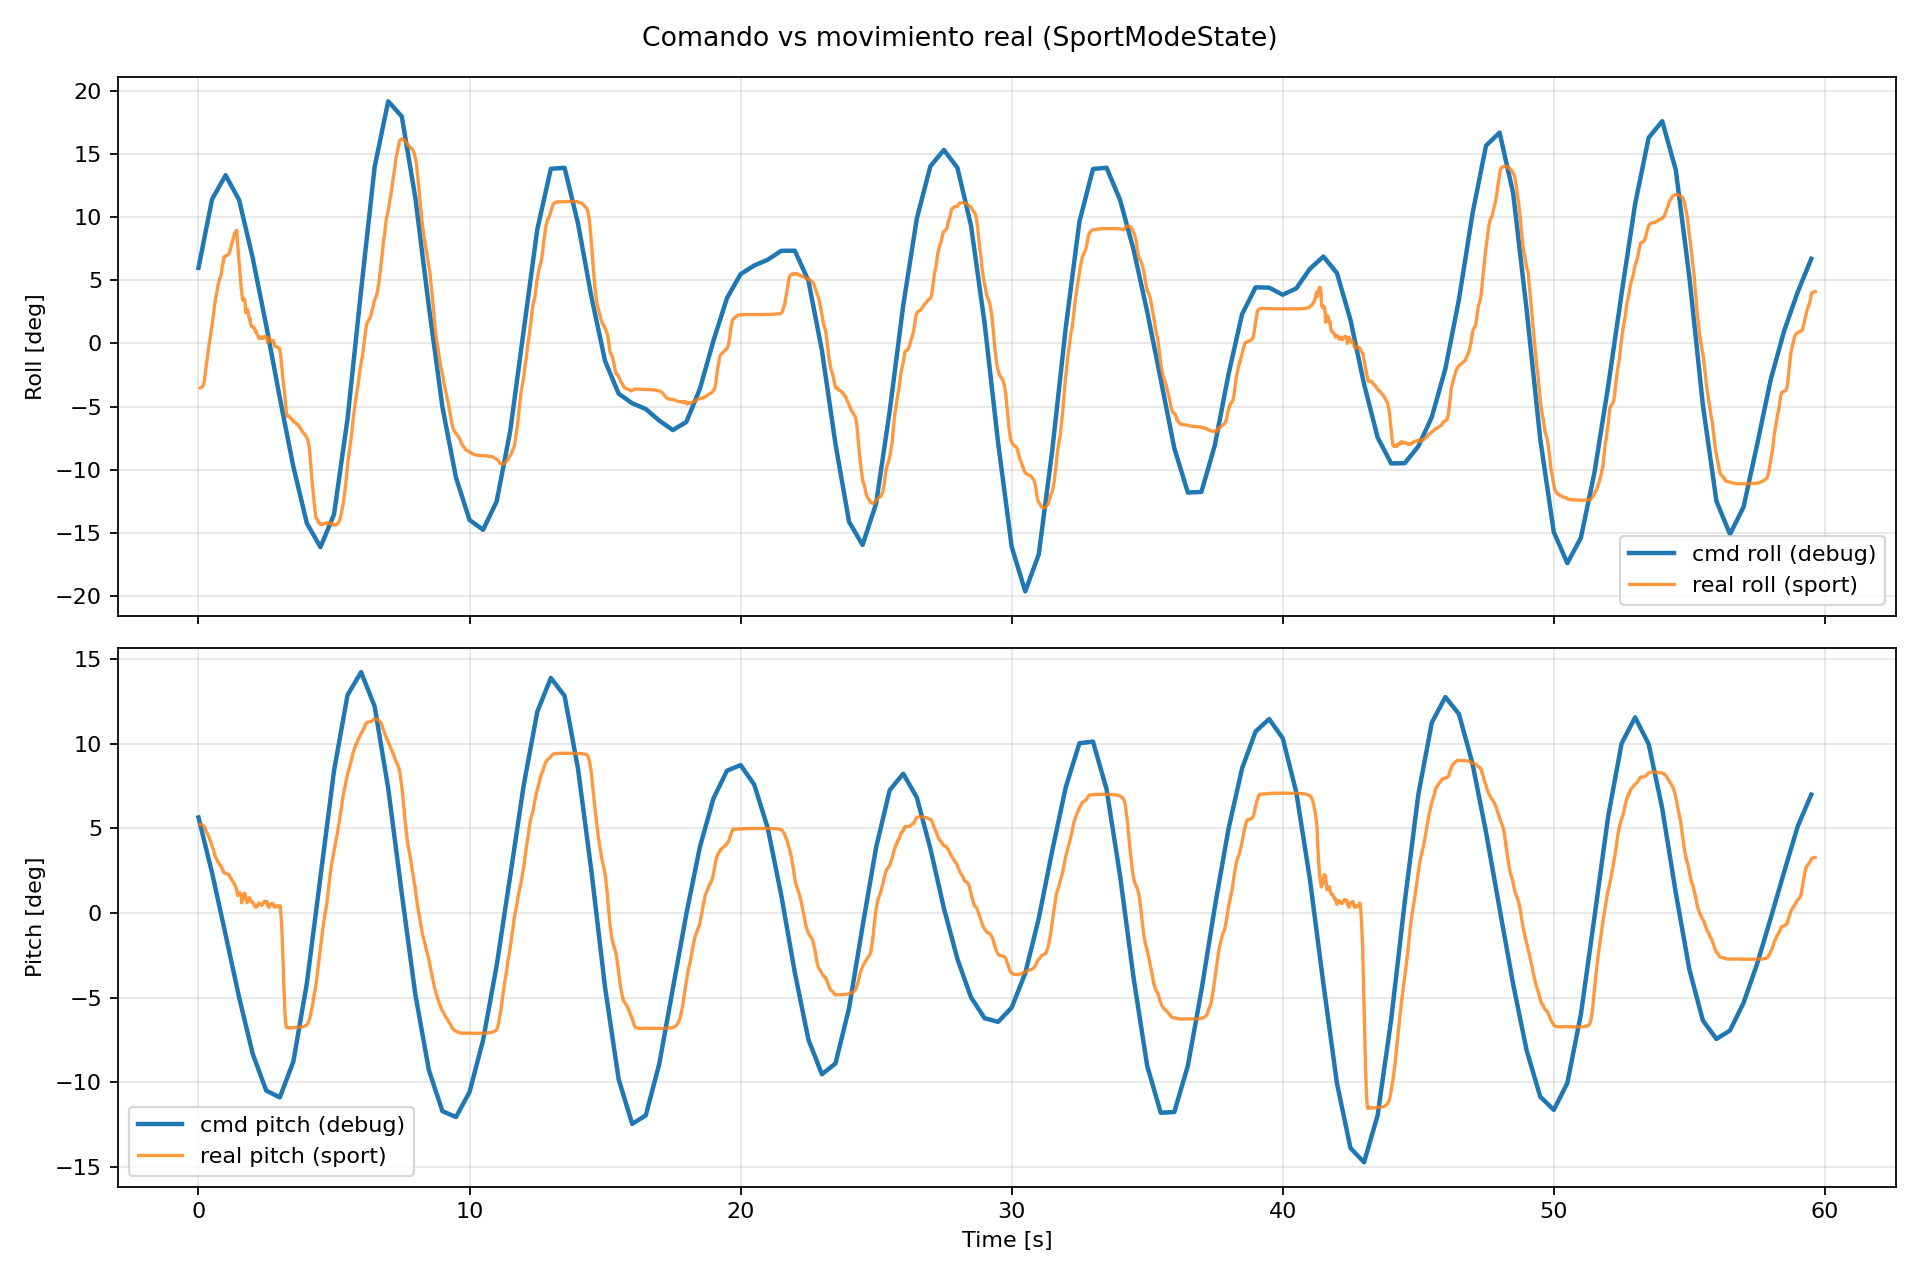
\includegraphics[width=\textwidth]{figures/images/lab_plot_01_timeseries_cmd_vs_real.png}
\caption{Comparación temporal entre movimiento esperado y respuesta del robot
real en laboratorio. Se muestran las consignas de \emph{roll} y \emph{pitch}
junto con la actitud reportada por el estado deportivo del Go2, lo que permite
leer forma general, amplitud efectiva y desfase temporal.}
\label{fig:lab_target_vs_odom}
\end{figure}

Los resultados muestran una coherencia alta entre objetivo y respuesta, aunque
no instantánea. A retardo cero, las correlaciones entre la señal esperada y la
respuesta real son del orden de \(0.91\) para roll y de \(0.81\) para pitch,
según la fuente de estado utilizada. Cuando se permite compensar el retardo del
sistema, la correspondencia mejora de manera marcada: la mejor correlación para
roll aparece alrededor de \texttt{0.35 s} y alcanza aproximadamente
\texttt{0.9695}, mientras que en pitch el mejor lag se ubica cerca de
\texttt{0.60 s}, con correlación cercana a \texttt{0.9680}. La lectura
experimental es clara: el robot reproduce la dinámica solicitada, pero lo hace
con retardo físico estable y con una amplitud efectiva algo menor que la de la
consigna.

Esta reducción de amplitud también aparece en los rangos de actitud medidos. En
el estado deportivo, el roll real varía entre \(-14.388^\circ\) y
\(16.190^\circ\), mientras que el pitch real recorre aproximadamente
\(-11.532^\circ\) a \(11.455^\circ\). No se trata de una falla del pipeline,
sino de una diferencia esperable entre pedir una oscilación ideal y obtener la
respuesta de un sistema físico con saturaciones, inercia, control interno y
restricciones de estabilidad. En este sentido, la evidencia del laboratorio no
busca mostrar coincidencia perfecta, sino demostrar que la plataforma real sigue
de manera consistente el movimiento propuesto.

\begin{figure}[H]
\centering
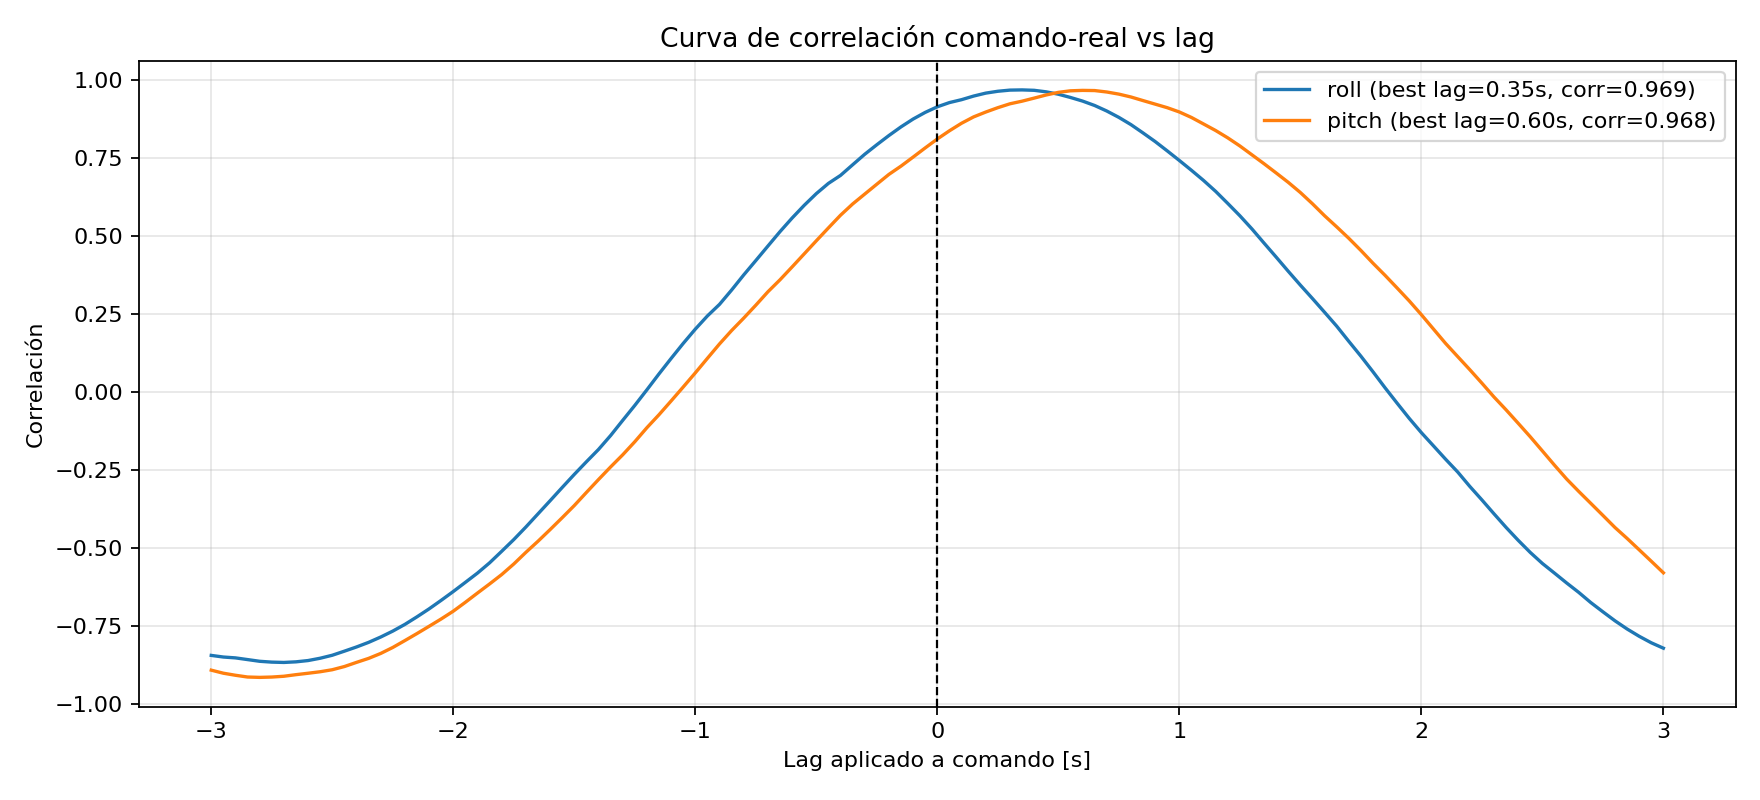
\includegraphics[width=\textwidth]{figures/images/lab_plot_03_lag_correlation.png}
\caption{Curvas de correlación entre comando y respuesta en función del retardo
aplicado a la señal esperada. La figura resume cómo mejora la correspondencia
entre la consigna y la actitud real del robot cuando se compensa el lag físico
del sistema.}
\label{fig:lab_lag_correlation}
\end{figure}

La comparación del eje vertical requiere una lectura aparte. En la corrida real
versionada, la señal esperada y la señal enviada al robot no incluyeron heave
dinámico: la coordenada vertical permaneció en cero tanto en la depuración del simulador marino como en las peticiones API. En
cambio, el estado real del robot sí presenta una coordenada vertical del tronco
alrededor de \texttt{0.32 m}, porque esa variable representa la altura absoluta
del cuerpo y no un desplazamiento relativo respecto de una referencia neutra.
Por eso, esta corrida no puede leerse como una validación de heave oscilatorio,
sino como una validación fuerte de roll y pitch con observación complementaria
de la altura del tronco.

\begin{figure}[H]
\centering
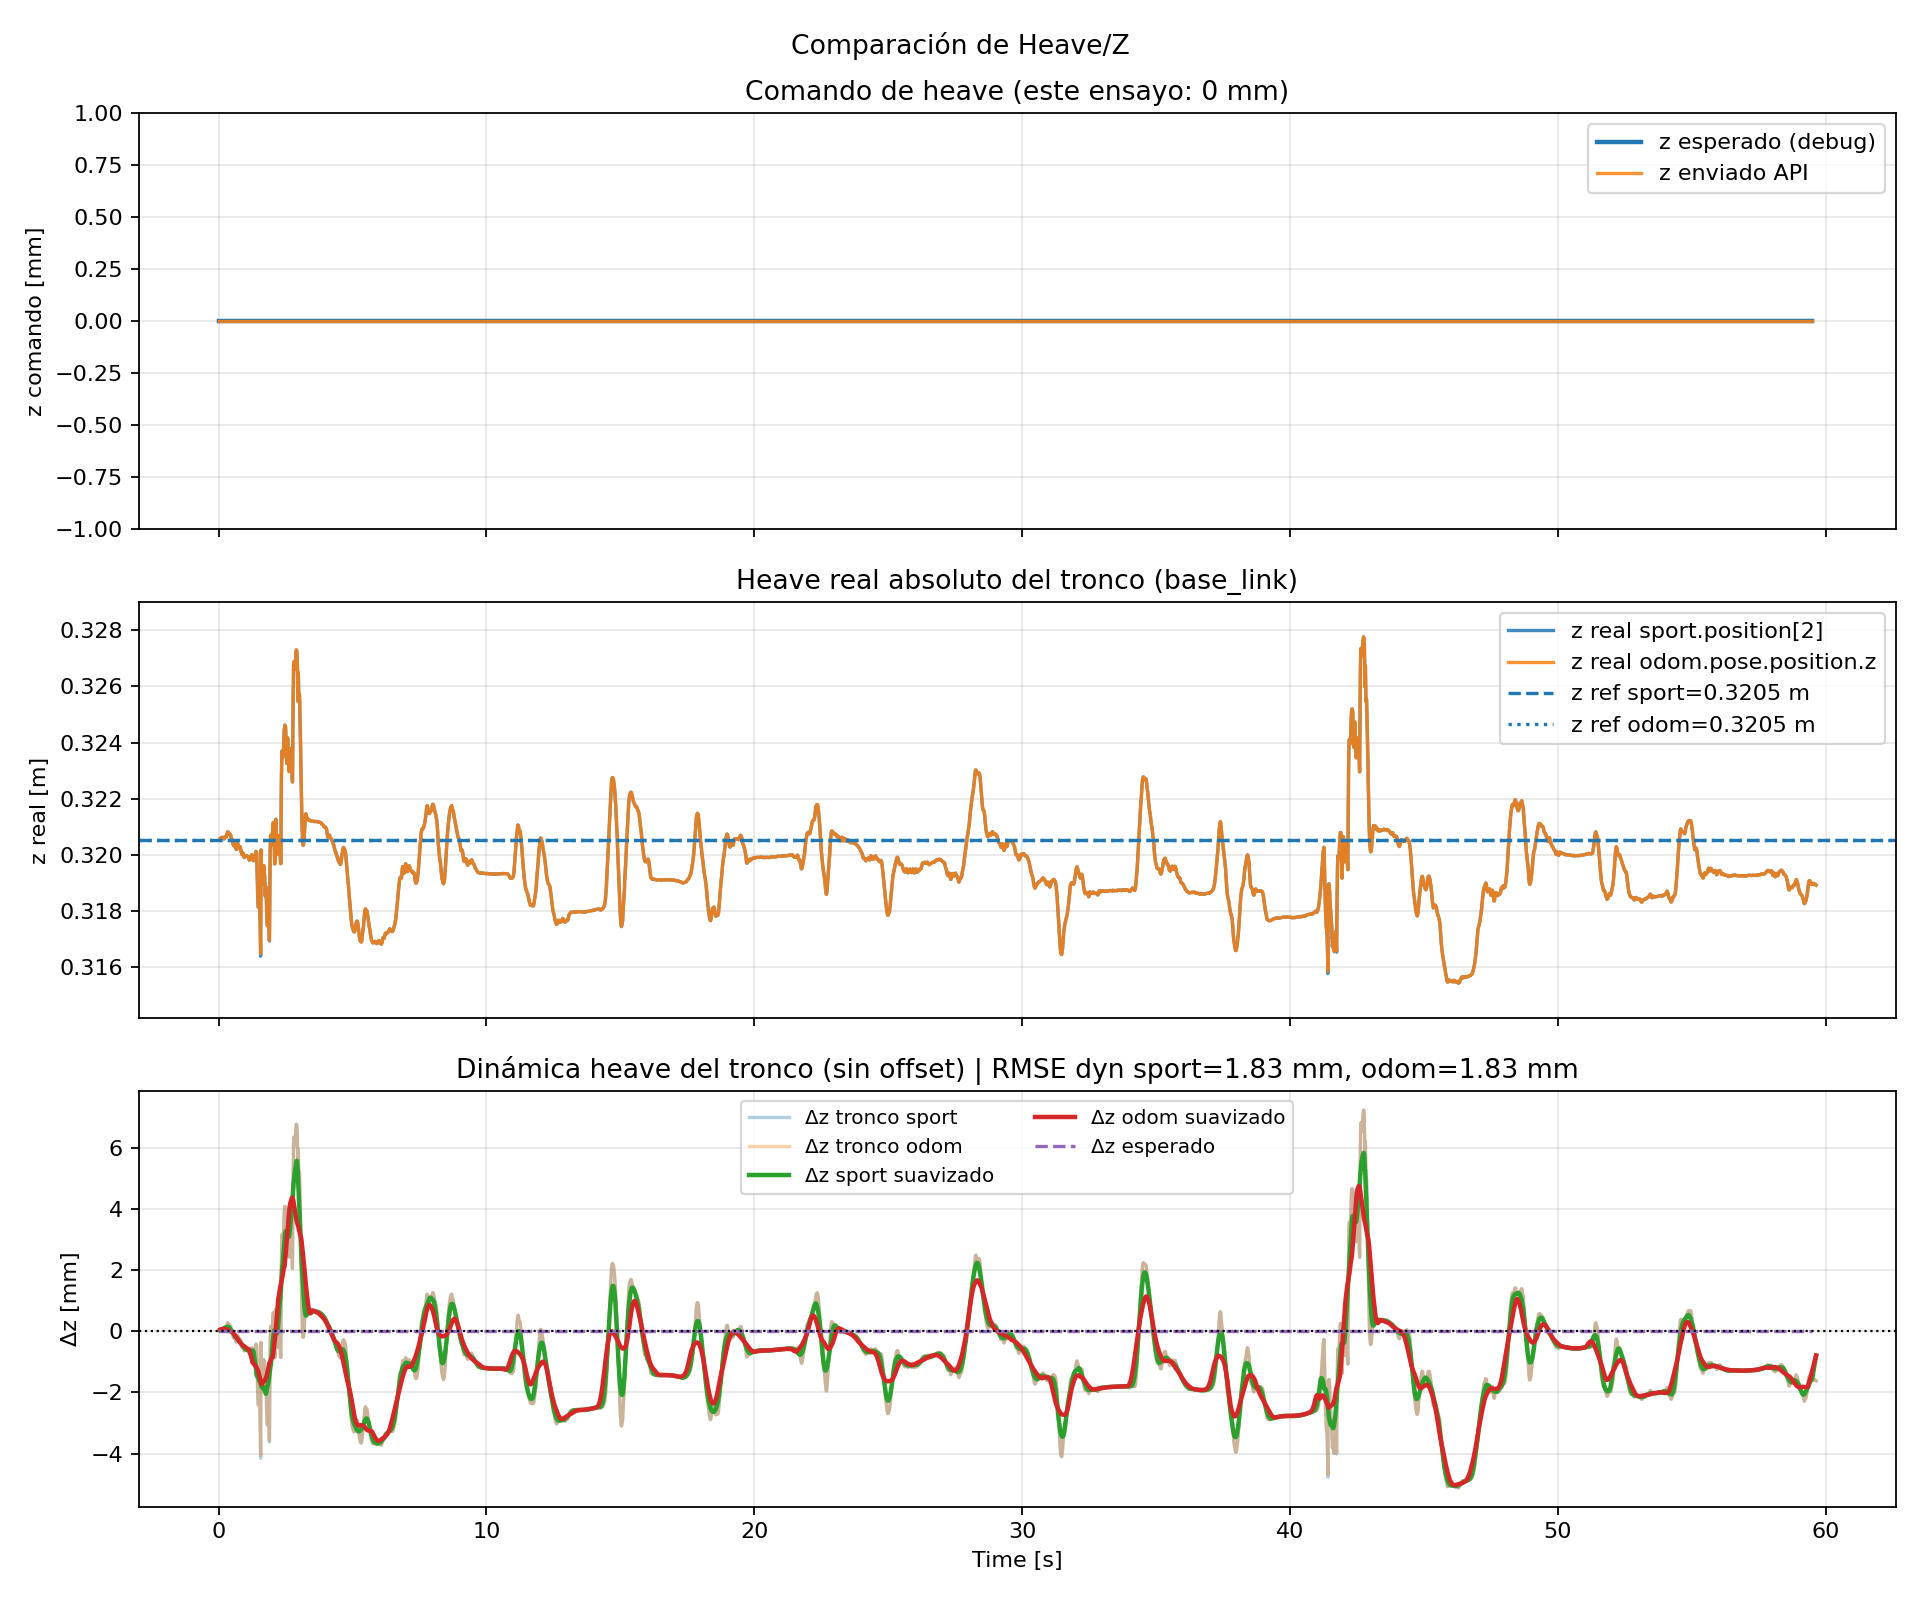
\includegraphics[width=\textwidth]{figures/images/lab_plot_05_heave_z_comparison.png}
\caption{Lectura del eje vertical en laboratorio. La figura distingue entre la
consigna de \emph{heave} enviada, la altura absoluta del tronco reportada por el
robot y la versión centrada de esa señal, para dejar explícito por qué esta
corrida no sostiene una comparación directa de \emph{heave} dinámico.}
\label{fig:lab_heave_comparison}
\end{figure}

\subsubsection{Lectura conjunta con la simulación}

Este cierre vincula la evidencia de laboratorio con la historia más amplia del
trabajo. No se trata de afirmar que ambos
entornos son idénticos, sino de mostrar si el comportamiento observado en el
laboratorio conserva rasgos suficientemente parecidos a los que motivaron la
plataforma sintética en Gazebo. Esa comparación es la que habilita a presentar
el framework no sólo como un entorno de simulación, sino como una herramienta
que guarda relación con un comportamiento físico plausible del cuadrúpedo.

La comparación con simulación muestra, en primer lugar, una coincidencia
importante en la forma del problema. En ambos entornos el núcleo experimental
consiste en pedir oscilaciones del cuerpo del Go2 y observar cómo esas
oscilaciones reaparecen en una señal medible. Lo que cambia no es el sentido del
experimento, sino el tipo de incertidumbre: en simulación dominan la geometría y
la evaluación contra ground truth; en laboratorio dominan el retardo dinámico,
las restricciones físicas del robot y el montaje del sensor real.

La evidencia versionada del laboratorio también obliga a matizar el alcance de
la comparación. La corrida principal no replica exactamente la configuración de
referencia de simulación: trabaja con una frecuencia dominante de
\texttt{0.15 Hz}, amplitudes cercanas a \(\pm 20^\circ\) en roll y
\(\pm 15^\circ\) en pitch, y sin heave dinámico efectivo. Aun así, su valor
metodológico es alto porque muestra que el movimiento sintetizado no era una
ficción puramente simulada: el robot real puede seguir consignas de esa clase de
forma estable, con alta coherencia temporal y un retardo razonablemente
constante.

En términos del objetivo general del trabajo, este resultado no valida todavía
un aterrizaje autónomo ni cierra por sí solo la estimación visual en entorno
real. Lo que sí hace es fortalecer el puente entre plataforma sintética,
percepción visual y comportamiento físico plausible del sistema. Esa continuidad
es justamente la condición necesaria para que el framework propuesto tenga valor
como etapa previa al estudio de aterrizaje de drones sobre plataformas marinas
móviles.



\section{Conclusiones}



\section{Trabajo futuro}

\appendix

\section{Identificadores de registros y archivos de datos}
\label{sec:appendix_data}

Este apéndice concentra \textbf{nombres de archivo} y \textbf{rutas relativas al
repositorio} citados en el documento. El cuerpo del texto prioriza campañas,
fechas y etiquetas (\(R1\)--\(R3\), baseline); aquí se deja la correspondencia
explícita para reproducibilidad.

\begin{table}[H]
\centering
\footnotesize
\caption{Registros ROS~2 (\texttt{rosbags}) mencionados en la experimentación.}
\label{tab:appendix_rosbags}
\begin{adjustbox}{max width=\textwidth}
\begin{tabular}{p{0.22\textwidth}p{0.50\textwidth}p{0.22\textwidth}}
\toprule
Referencia en el texto & Nombre base del archivo & Notas \\
\midrule
Baseline sim.\ cámara fija & \path{marine_sim_20260410_155332_report_v2_ref} & Campaña \texttt{report\_v2}; $\sim 57{,}5$~s \\
Corrida \(R1\) (dron) & \path{sjtu_drone_sim_20260410_155834_report_v2_r1} & idem \\
Corrida \(R2\) (dron) & \path{sjtu_drone_sim_20260410_160419_report_v2_r2} & idem \\
Corrida \(R3\) (dron) & \path{sjtu_drone_sim_20260410_160814_report_v2_r3} & idem \\
Laboratorio (referencia) & \path{lab_real_20260320_125002_movimiento_full_v3} & 20-03-2026; $\sim 59{,}73$~s \\
\bottomrule
\end{tabular}
\end{adjustbox}
\end{table}

\noindent\textbf{Archivos de cámara estéreo (laboratorio).} La configuración del
publicador y el resultado de calibración utilizados en las pruebas versionadas
se encuentran, respectivamente, en \path{stereo_camera/config.yaml} y
\path{stereo_camera/calibration/calibration_result.yaml} dentro del paquete
del publicador de imagen en el repositorio.

% \begin{landscape}
%     \input{regressions/regression}
% \end{landscape}

% \begin{landscape}
%     \input{regressions/heterogeneity}
% \end{landscape}

\section{Bibliografía}
\printbibliography[heading=none]

\end{document}
